\documentclass{article}
\usepackage[font=small,labelfont=bf]{caption} % Required for specifying captions to tables and figures
\usepackage{graphicx}

\usepackage{hyperref}

\usepackage{sectsty}
\graphicspath{ {./images/} }

%%%%%%%%%%%%%%%%%%%%%%%%%%%%%%%%%%%%%%%%%
% Lachaise Assignment
% Structure Specification File
% Version 1.0 (26/6/2018)
%
% This template originates from:
% http://www.LaTeXTemplates.com
%
% Authors:
% Marion Lachaise & François Févotte
% Vel (vel@LaTeXTemplates.com)
%
% License:
% CC BY-NC-SA 3.0 (http://creativecommons.org/licenses/by-nc-sa/3.0/)
% 
%%%%%%%%%%%%%%%%%%%%%%%%%%%%%%%%%%%%%%%%%

%----------------------------------------------------------------------------------------
%	PACKAGES AND OTHER DOCUMENT CONFIGURATIONS
%----------------------------------------------------------------------------------------

\usepackage{amsmath,amsfonts,stmaryrd,amssymb} % Math packages

\usepackage{enumerate} % Custom item numbers for enumerations

\usepackage[ruled]{algorithm2e} % Algorithms

\usepackage[framemethod=tikz]{mdframed} % Allows defining custom boxed/framed environments

\usepackage{listings} % File listings, with syntax highlighting
\lstset{
	basicstyle=\ttfamily, % Typeset listings in monospace font
}

%----------------------------------------------------------------------------------------
%	DOCUMENT MARGINS
%----------------------------------------------------------------------------------------

\usepackage{geometry} % Required for adjusting page dimensions and margins

\geometry{
	paper=a4paper, % Paper size, change to letterpaper for US letter size
	top=2.5cm, % Top margin
	bottom=3cm, % Bottom margin
	left=2.5cm, % Left margin
	right=2.5cm, % Right margin
	headheight=14pt, % Header height
	footskip=1.5cm, % Space from the bottom margin to the baseline of the footer
	headsep=1.2cm, % Space from the top margin to the baseline of the header
	%showframe, % Uncomment to show how the type block is set on the page
}

%----------------------------------------------------------------------------------------
%	FONTS
%----------------------------------------------------------------------------------------

\usepackage[utf8]{inputenc} % Required for inputting international characters
\usepackage[T1]{fontenc} % Output font encoding for international characters

\usepackage{XCharter} % Use the XCharter fonts

%----------------------------------------------------------------------------------------
%	COMMAND LINE ENVIRONMENT
%----------------------------------------------------------------------------------------

% Usage:
% \begin{commandline}
%	\begin{verbatim}
%		$ ls
%		
%		Applications	Desktop	...
%	\end{verbatim}
% \end{commandline}

\mdfdefinestyle{commandline}{
	leftmargin=10pt,
	rightmargin=10pt,
	innerleftmargin=15pt,
	middlelinecolor=black!50!white,
	middlelinewidth=2pt,
	frametitlerule=false,
	backgroundcolor=black!5!white,
	frametitle={Command Line},
	frametitlefont={\normalfont\sffamily\color{white}\hspace{-1em}},
	frametitlebackgroundcolor=black!50!white,
	nobreak,
}

% Define a custom environment for command-line snapshots
\newenvironment{commandline}{
	\medskip
	\begin{mdframed}[style=commandline]
}{
	\end{mdframed}
	\medskip
}

%----------------------------------------------------------------------------------------
%	FILE CONTENTS ENVIRONMENT
%----------------------------------------------------------------------------------------

% Usage:
% \begin{file}[optional filename, defaults to "File"]
%	File contents, for example, with a listings environment
% \end{file}

\mdfdefinestyle{file}{
	innertopmargin=1.6\baselineskip,
	innerbottommargin=0.8\baselineskip,
	topline=false, bottomline=false,
	leftline=false, rightline=false,
	leftmargin=2cm,
	rightmargin=2cm,
	singleextra={%
		\draw[fill=black!10!white](P)++(0,-1.2em)rectangle(P-|O);
		\node[anchor=north west]
		at(P-|O){\ttfamily\mdfilename};
		%
		\def\l{3em}
		\draw(O-|P)++(-\l,0)--++(\l,\l)--(P)--(P-|O)--(O)--cycle;
		\draw(O-|P)++(-\l,0)--++(0,\l)--++(\l,0);
	},
	nobreak,
}

% Define a custom environment for file contents
\newenvironment{file}[1][File]{ % Set the default filename to "File"
	\medskip
	\newcommand{\mdfilename}{#1}
	\begin{mdframed}[style=file]
}{
	\end{mdframed}
	\medskip
}

%----------------------------------------------------------------------------------------
%	NUMBERED QUESTIONS ENVIRONMENT
%----------------------------------------------------------------------------------------

% Usage:
% \begin{question}[optional title]
%	Question contents
% \end{question}

\mdfdefinestyle{question}{
	innertopmargin=1.2\baselineskip,
	innerbottommargin=0.8\baselineskip,
	roundcorner=5pt,
	nobreak,
	singleextra={%
		\draw(P-|O)node[xshift=1em,anchor=west,fill=white,draw,rounded corners=5pt]{%
		Question \theQuestion\questionTitle};
	},
}

\newcounter{Question} % Stores the current question number that gets iterated with each new question

% Define a custom environment for numbered questions
\newenvironment{question}[1][\unskip]{
	\bigskip
	\stepcounter{Question}
	\newcommand{\questionTitle}{~#1}
	\begin{mdframed}[style=question]
}{
	\end{mdframed}
	\medskip
}

%----------------------------------------------------------------------------------------
%	WARNING TEXT ENVIRONMENT
%----------------------------------------------------------------------------------------

% Usage:
% \begin{warn}[optional title, defaults to "Warning:"]
%	Contents
% \end{warn}

\mdfdefinestyle{warning}{
	topline=false, bottomline=false,
	leftline=false, rightline=false,
	nobreak,
	singleextra={%
		\draw(P-|O)++(-0.5em,0)node(tmp1){};
		\draw(P-|O)++(0.5em,0)node(tmp2){};
		\fill[black,rotate around={45:(P-|O)}](tmp1)rectangle(tmp2);
		\node at(P-|O){\color{white}\scriptsize\bf !};
		\draw[very thick](P-|O)++(0,-1em)--(O);%--(O-|P);
	}
}

% Define a custom environment for warning text
\newenvironment{warn}[1][Warning:]{ % Set the default warning to "Warning:"
	\medskip
	\begin{mdframed}[style=warning]
		\noindent{\textbf{#1}}
}{
	\end{mdframed}
}

%----------------------------------------------------------------------------------------
%	INFORMATION ENVIRONMENT
%----------------------------------------------------------------------------------------

% Usage:
% \begin{info}[optional title, defaults to "Info:"]
% 	contents
% 	\end{info}

\mdfdefinestyle{info}{%
	topline=false, bottomline=false,
	leftline=false, rightline=false,
	nobreak,
	singleextra={%
		\fill[black](P-|O)circle[radius=0.4em];
		\node at(P-|O){\color{white}\scriptsize\bf i};
		\draw[very thick](P-|O)++(0,-0.8em)--(O);%--(O-|P);
	}
}

% Define a custom environment for information
\newenvironment{info}[1][Info:]{ % Set the default title to "Info:"
	\medskip
	\begin{mdframed}[style=info]
		\noindent{\textbf{#1}}
}{
	\end{mdframed}
}
 % Include the file specifying the document structure and custom commands

%----------------------------------------------------------------------------------------
%	ASSIGNMENT INFORMATION
%----------------------------------------------------------------------------------------

\title{ %

\includegraphics[width=0.4\textwidth]{UniCT-Logo-Nero}~\\
BiobankSPREC Microservices \\ 
\large Progetto Sistemi Cloud e Laboratorio (LM-18) \\ Università degli Studi di Catania - A.A 2021/2022 \\
}
\author{ Danilo Leocata - 1000022576 \\ Alessio Angelo Liotta - 1000012434 \\Docenti: Giuseppe Pappalardo, Andrea Fornaia}
\date{\today}

%----------------------------------------------------------------------------------------

\begin{document}

\maketitle % Print the title

\pagebreak

%----------------------------------------------------------------------------------------
%	INTRODUCTION
%----------------------------------------------------------------------------------------


\section{Introduzione}

È stato preso in esame un progetto a microservizi realizzato precedentemente. Il dominio del problema proposto è un sistema (Biobanca) che si occupa di
memorizzare i dati relativi a campioni biologici.
Tale sistema oltre ad occuparsi della memorizzazione delle informazionisui campioni
biologici, implementa l’autenticazione e il controllo degli accessi (quindi avremo
tabelle come utenti, ruoli e permessi associati), la gestione delle spedizioni dei
campioni biologici, l’archiviazione delle informazioni sui donatori e le
informazioni sulla biobanca stessa (ad esempio, dove verranno conservati i campioni
veri e propri). L'intero progetto è disponibile al seguente link GitHub: \href{https://github.com/sistemi-cloud-2022}{https://github.com/sistemi-cloud-2022}.

\begin{center}
    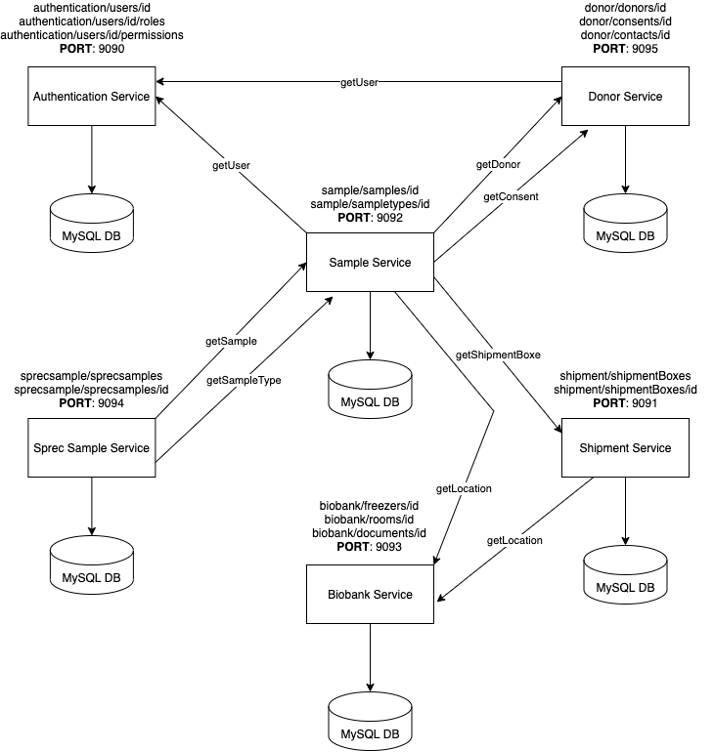
\includegraphics[width=0.6\linewidth]{architettura.png}
    \captionof{figure}{Architettura iniziale}
\end{center}


È stato trovato più opportuno, iniziare ad effettuare un primo refactoring del progetto.
In particolare è stata prevista la suddivisione dei microservizi, ed i relativi database, in repository separate in modo da scindere il deploy di database e relativo microservizio associato.
Le referenze dei tool descritti nella seguente relazione sono stati inseriti nel capitolo delle references.
Tutte le configurazioni (come quella di Keycloak, ad esempio) e le documentazioni generali sono state inserite all’interno della repository \texttt{main}. Per agevolare lo sviluppo ed i test sono stati implementati due script bash, nel dettaglio:

\begin{enumerate}
    \item {\texttt{setup-dev.sh}: crea una cartella \texttt{development}, al cui interno effettua i clone delle repository, prepara i file in modo da renderli eseguibili per il \texttt{docker-compose}, effettua la build del microservizi con \texttt{maven} e
        copia tutti i file necessari per la configurazione  dentro la cartella \texttt{imports}};
    \item {\texttt{update-repo.sh}: script che effettua pull del \texttt{main} in tutti i branch e ne effettua le build}.
\end{enumerate}

In generale, sono stati effettuati i seguenti miglioramenti su ogni microservizio:

\begin{enumerate}
    \item {Il microservizio di authentication è stato sostituito in favore di Keycloak; }
    \item {Sono stati estratti, dai rispettivi container docker, le tabelle ed i dati su file \texttt{.sql} (inizialmente il db veniva inizializzato a run-time durante l'avvio del microservizio);}
    \item {I file \texttt{pom.xml} sono stati stato revisionati ed aggiornati;}
    \item {Il formato delle API è stato cambiato da \textit{camelCase} ad \textit{hypenate}}
    \item {Per ogni repository è stato implementato un \texttt{docker-compose.yaml}}
    \item {I file \texttt{application.properties} sono stati stato convertiti in formato \texttt{.yml} e splittato in \texttt{dev}, per lo sviluppo, e \texttt{prod} per il deploy.}
    \item {Sono state implementate le \textbf{Git Actions} }
    \item {Orchestrazione dei microservizi con \textbf{Kubernetes}}
\end{enumerate}


\section{Keycloak}

% TODO: Viene utilizzato un DB mysql per il Docker-compose mentre un H2 di default per il deploy con k8s.

Il primo step è stato quello di sostituire il microservizio di autenticazione con Keyacloak. Keycloak è un
prodotto software open source che abilita il Single Sign-On (IdP) con Identity Management e
Access Management per applicazioni e servizi moderni. Questo software è scritto in Java e
supporta i protocolli di federazione delle identità per impostazione predefinita SAML v2 e
OpenID Connect (OIDC) / OAuth2. Lo scopo dello strumento è quello di facilitare la protezione
di applicazioni e servizi con poca o nessuna crittografia. Un IdP consente a un'applicazione
(Service Provider) di delegare la propria autenticazione %%(\href{https://www.keycloak.org}{pagina ufficiale}).

Si riassumono brevemente alcuni dei concetti principali:

\begin{enumerate}
    \item {\textbf{Users}: entità che sono in grado di accedere al tuo sistema. Possono avere attributi associati a se stessi come e-mail, nome utente, indirizzo, numero di telefono e giorno di nascita. È possibile assegnare loro l'appartenenza a un gruppo e assegnare loro ruoli specifici.}
    \item {\textbf{Roles}: identificano un tipo o una categoria di utente: sono tutti ruoli tipici che possono esistere in un'organizzazione. Le applicazioni spesso assegnano l'accesso e le autorizzazioni a ruoli specifici piuttosto che a singoli utenti, poiché la gestione degli utenti può essere difficile da gestire. }
    \item {\textbf{User role mapping} Una mappatura dei ruoli utente definisce una mappatura tra un ruolo e un utente. Un utente può essere associato a zero o più ruoli. Queste informazioni sulla mappatura dei ruoli possono essere incapsulate in token e asserzioni in modo che le applicazioni possano decidere le autorizzazioni di accesso su varie risorse che gestiscono.}
    \item {\textbf{Realms} un realm gestisce un insieme di utenti, credenziali, ruoli e gruppi. Un utente appartiene e accede a un realm che sono isolati l'uno dall'altro e possono solo gestire e autenticare gli utenti che controllano.}
    \item {\textbf{Clients}: i client sono entità che possono richiedere a Keycloak di autenticare un utente. Nella maggior parte dei casi, i client sono applicazioni e servizi che desiderano utilizzare Keycloak per proteggersi e fornire una soluzione single sign-on. I client possono anche essere entità che desiderano semplicemente richiedere informazioni sull'identità o un token di accesso in modo da poter invocare in modo sicuro altri servizi sulla rete protetti da Keycloak.}
    \item {\textbf{Client scope}: quando un client viene registrato, è necessario definire i mappatori di protocollo e i mapping dell'ambito del ruolo per quel client. Spesso è utile memorizzare un ambito client per semplificare la creazione di nuovi client condividendo alcune impostazioni comuni, è utile anche per richiedere che alcuni ruoli, ad esempio, siano condizionalmente basati sul valore del parametro scope}
    \item {\textbf{Client role}: i clients possono definire ruoli specifici.}
\end{enumerate}

Di seguito, saranno spiegati brevemente i passi necessari per la configurazione di Keycloak. Si nota che nel README del \textit{main} è presente una breve introduzione per avviare Keycloak in locale utilizzando docker.

\subsection{Creazione di un realm}

Dirigersi sull'indirizzo di Keycloak, nel nostro caso \texttt{http://localhost:8180/}

\begin{center}
    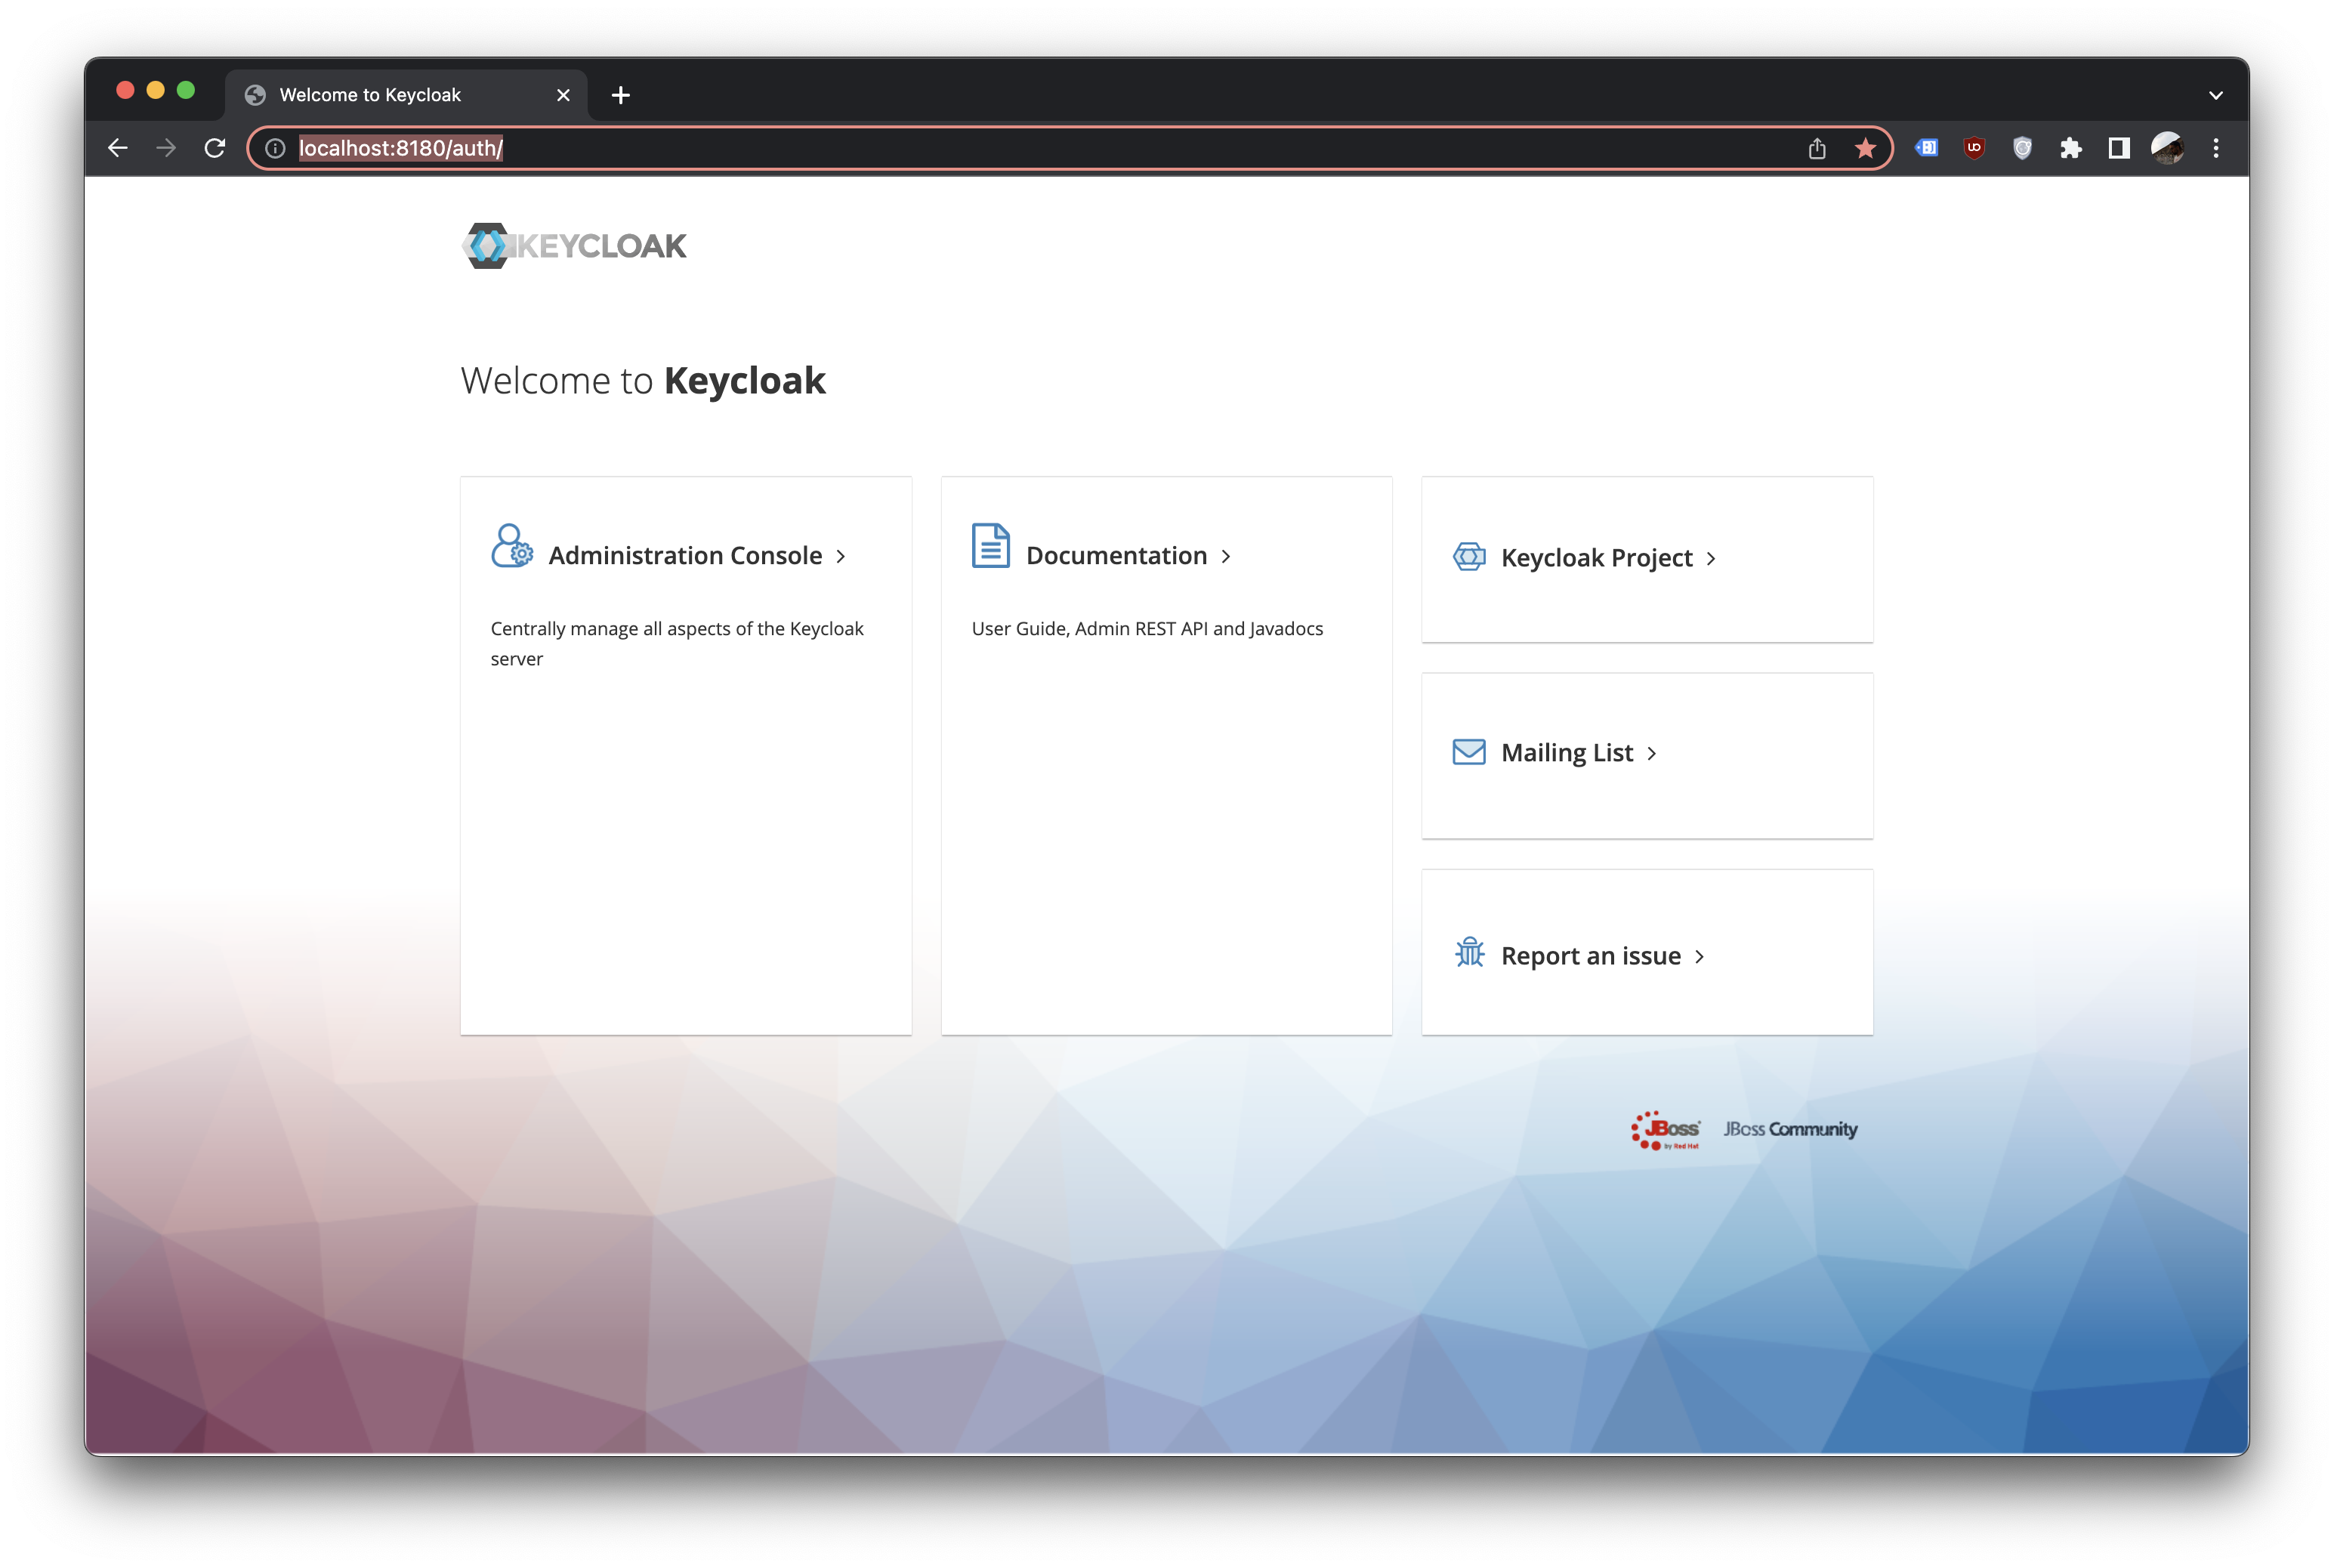
\includegraphics[width=0.80\linewidth]{keycloak_01.png}
\end{center}

Cliccare su \textit{administration console} ed effettuare la login con le credenziali dell'utente di amministrazione. In basso
troviamo la pagina iniziale.

\begin{center}
    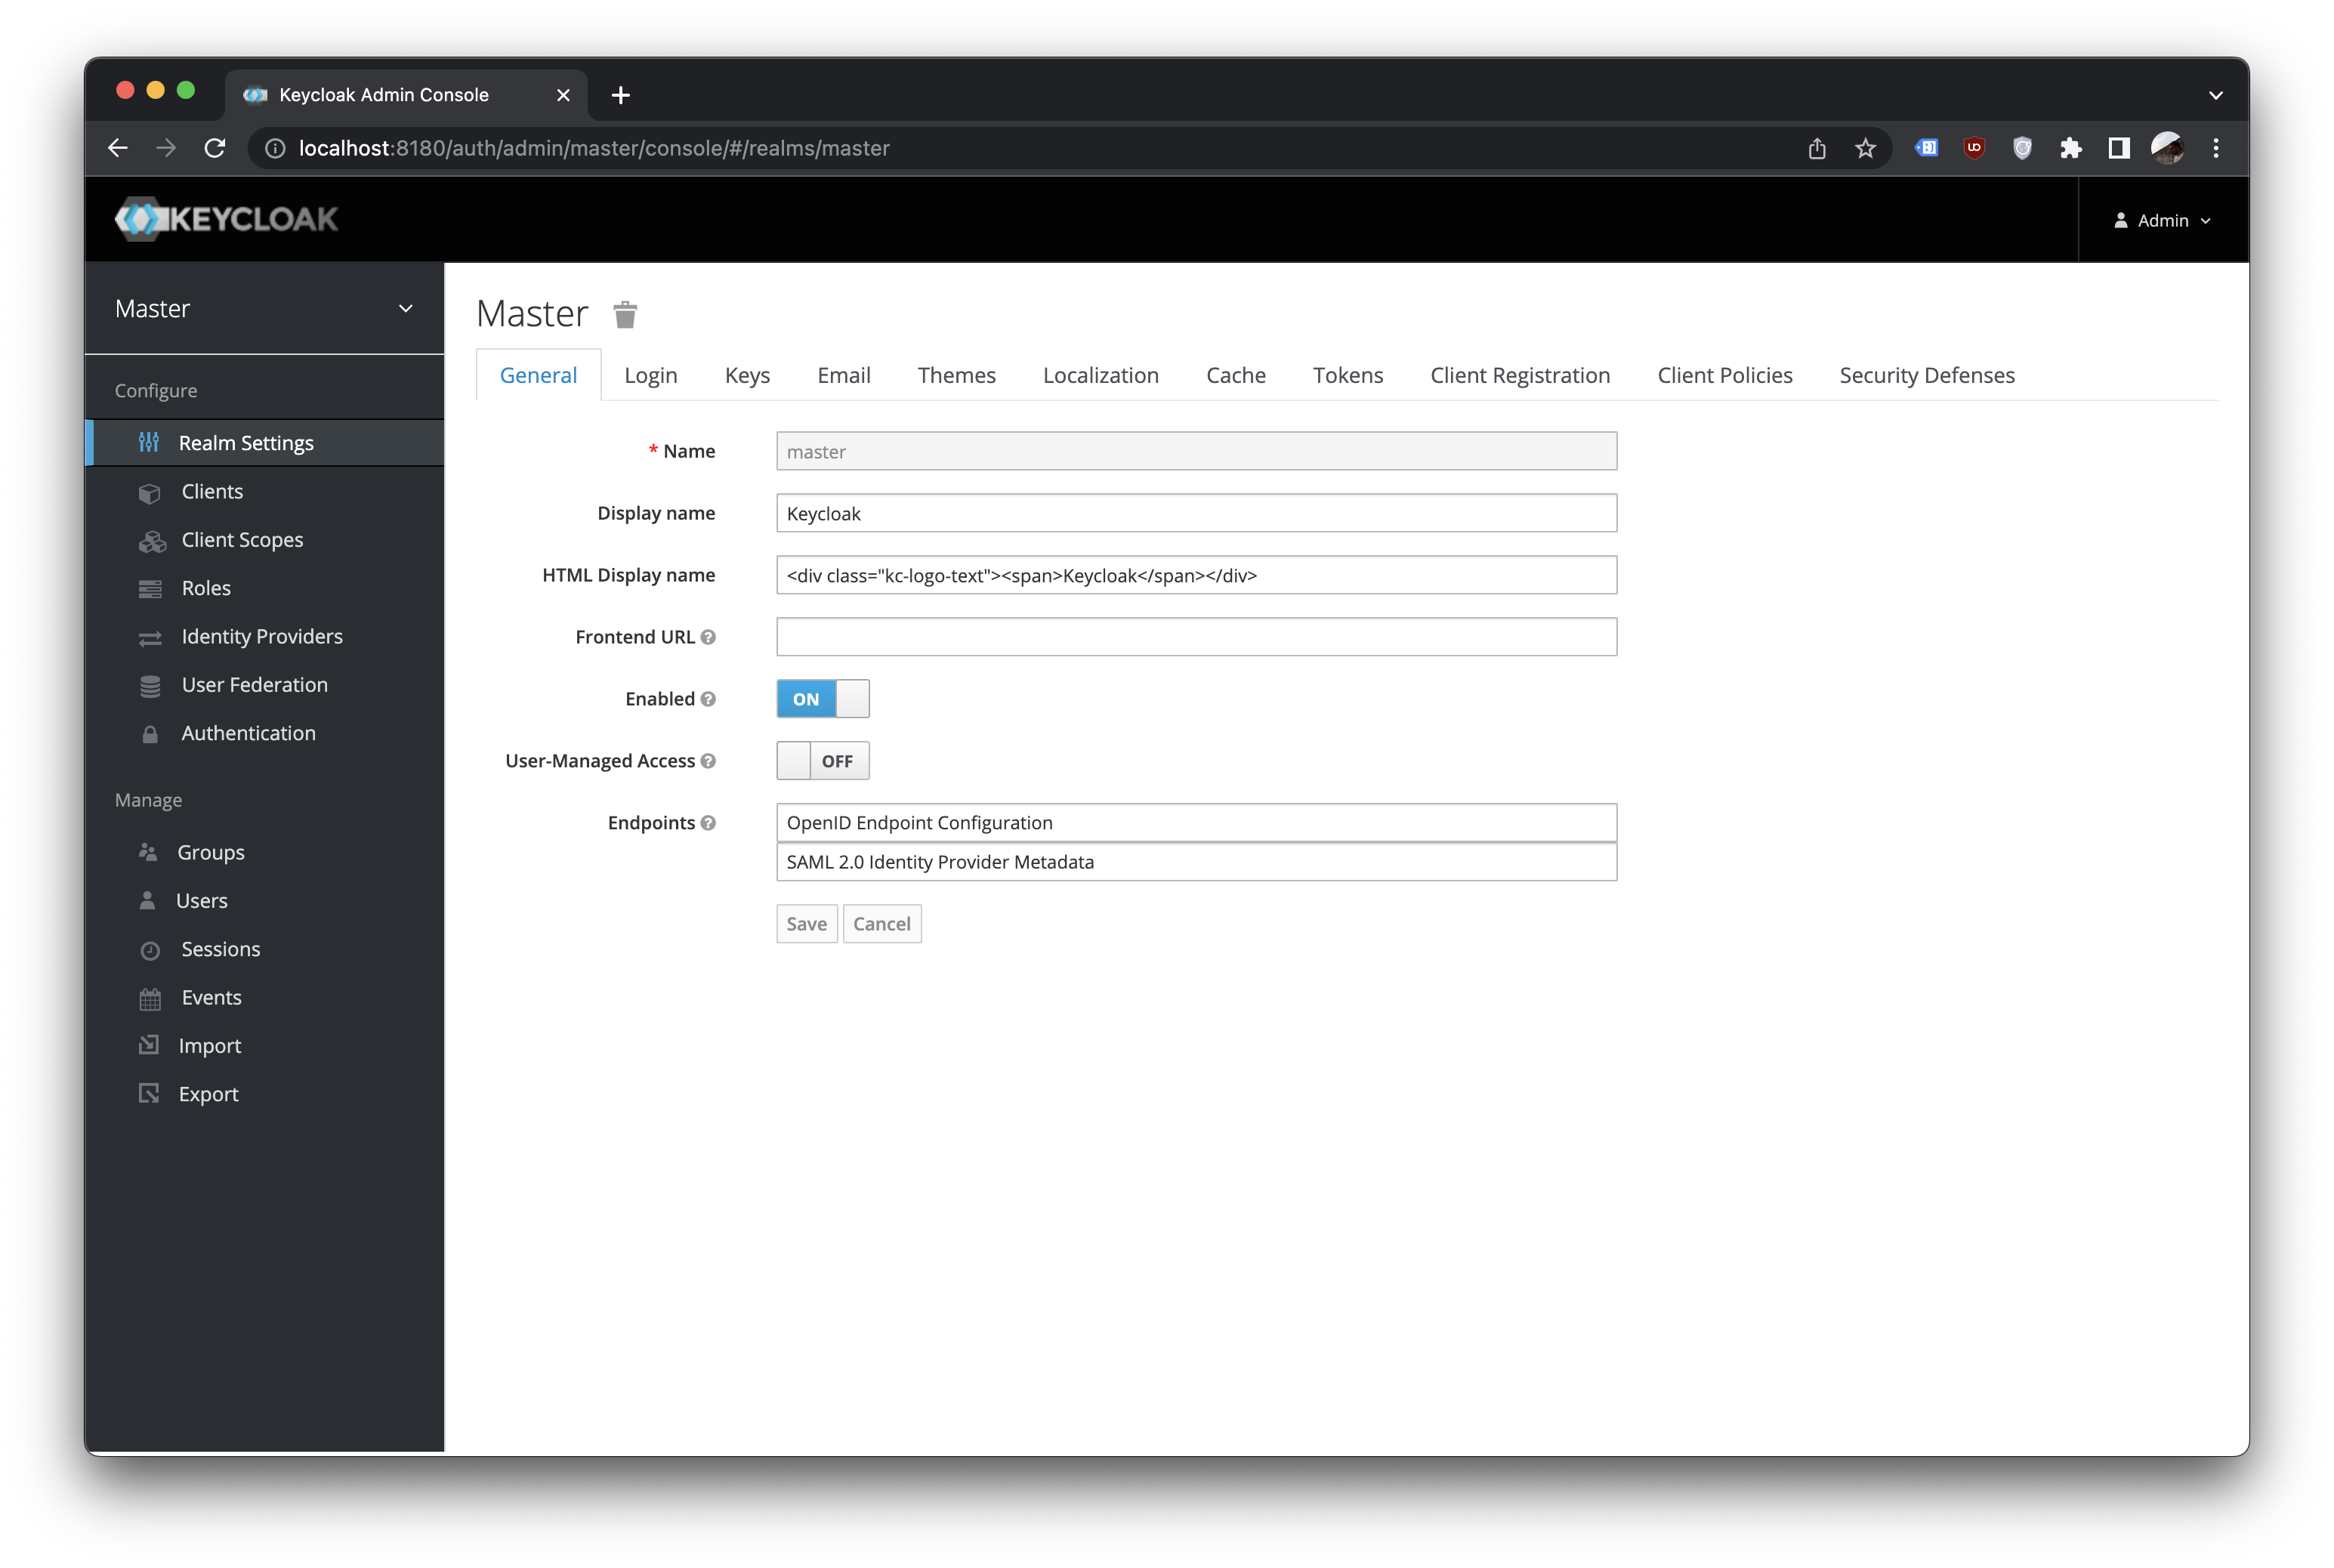
\includegraphics[width=0.80\linewidth]{keycloak_02.png}
\end{center}

Dirigiamogi con il cursore su \texttt{Master}: apparirà un menù a tendina che comprenderà l'elenco dei realm già creati e un bottone che darà la possibilità di crearli.

\begin{center}
    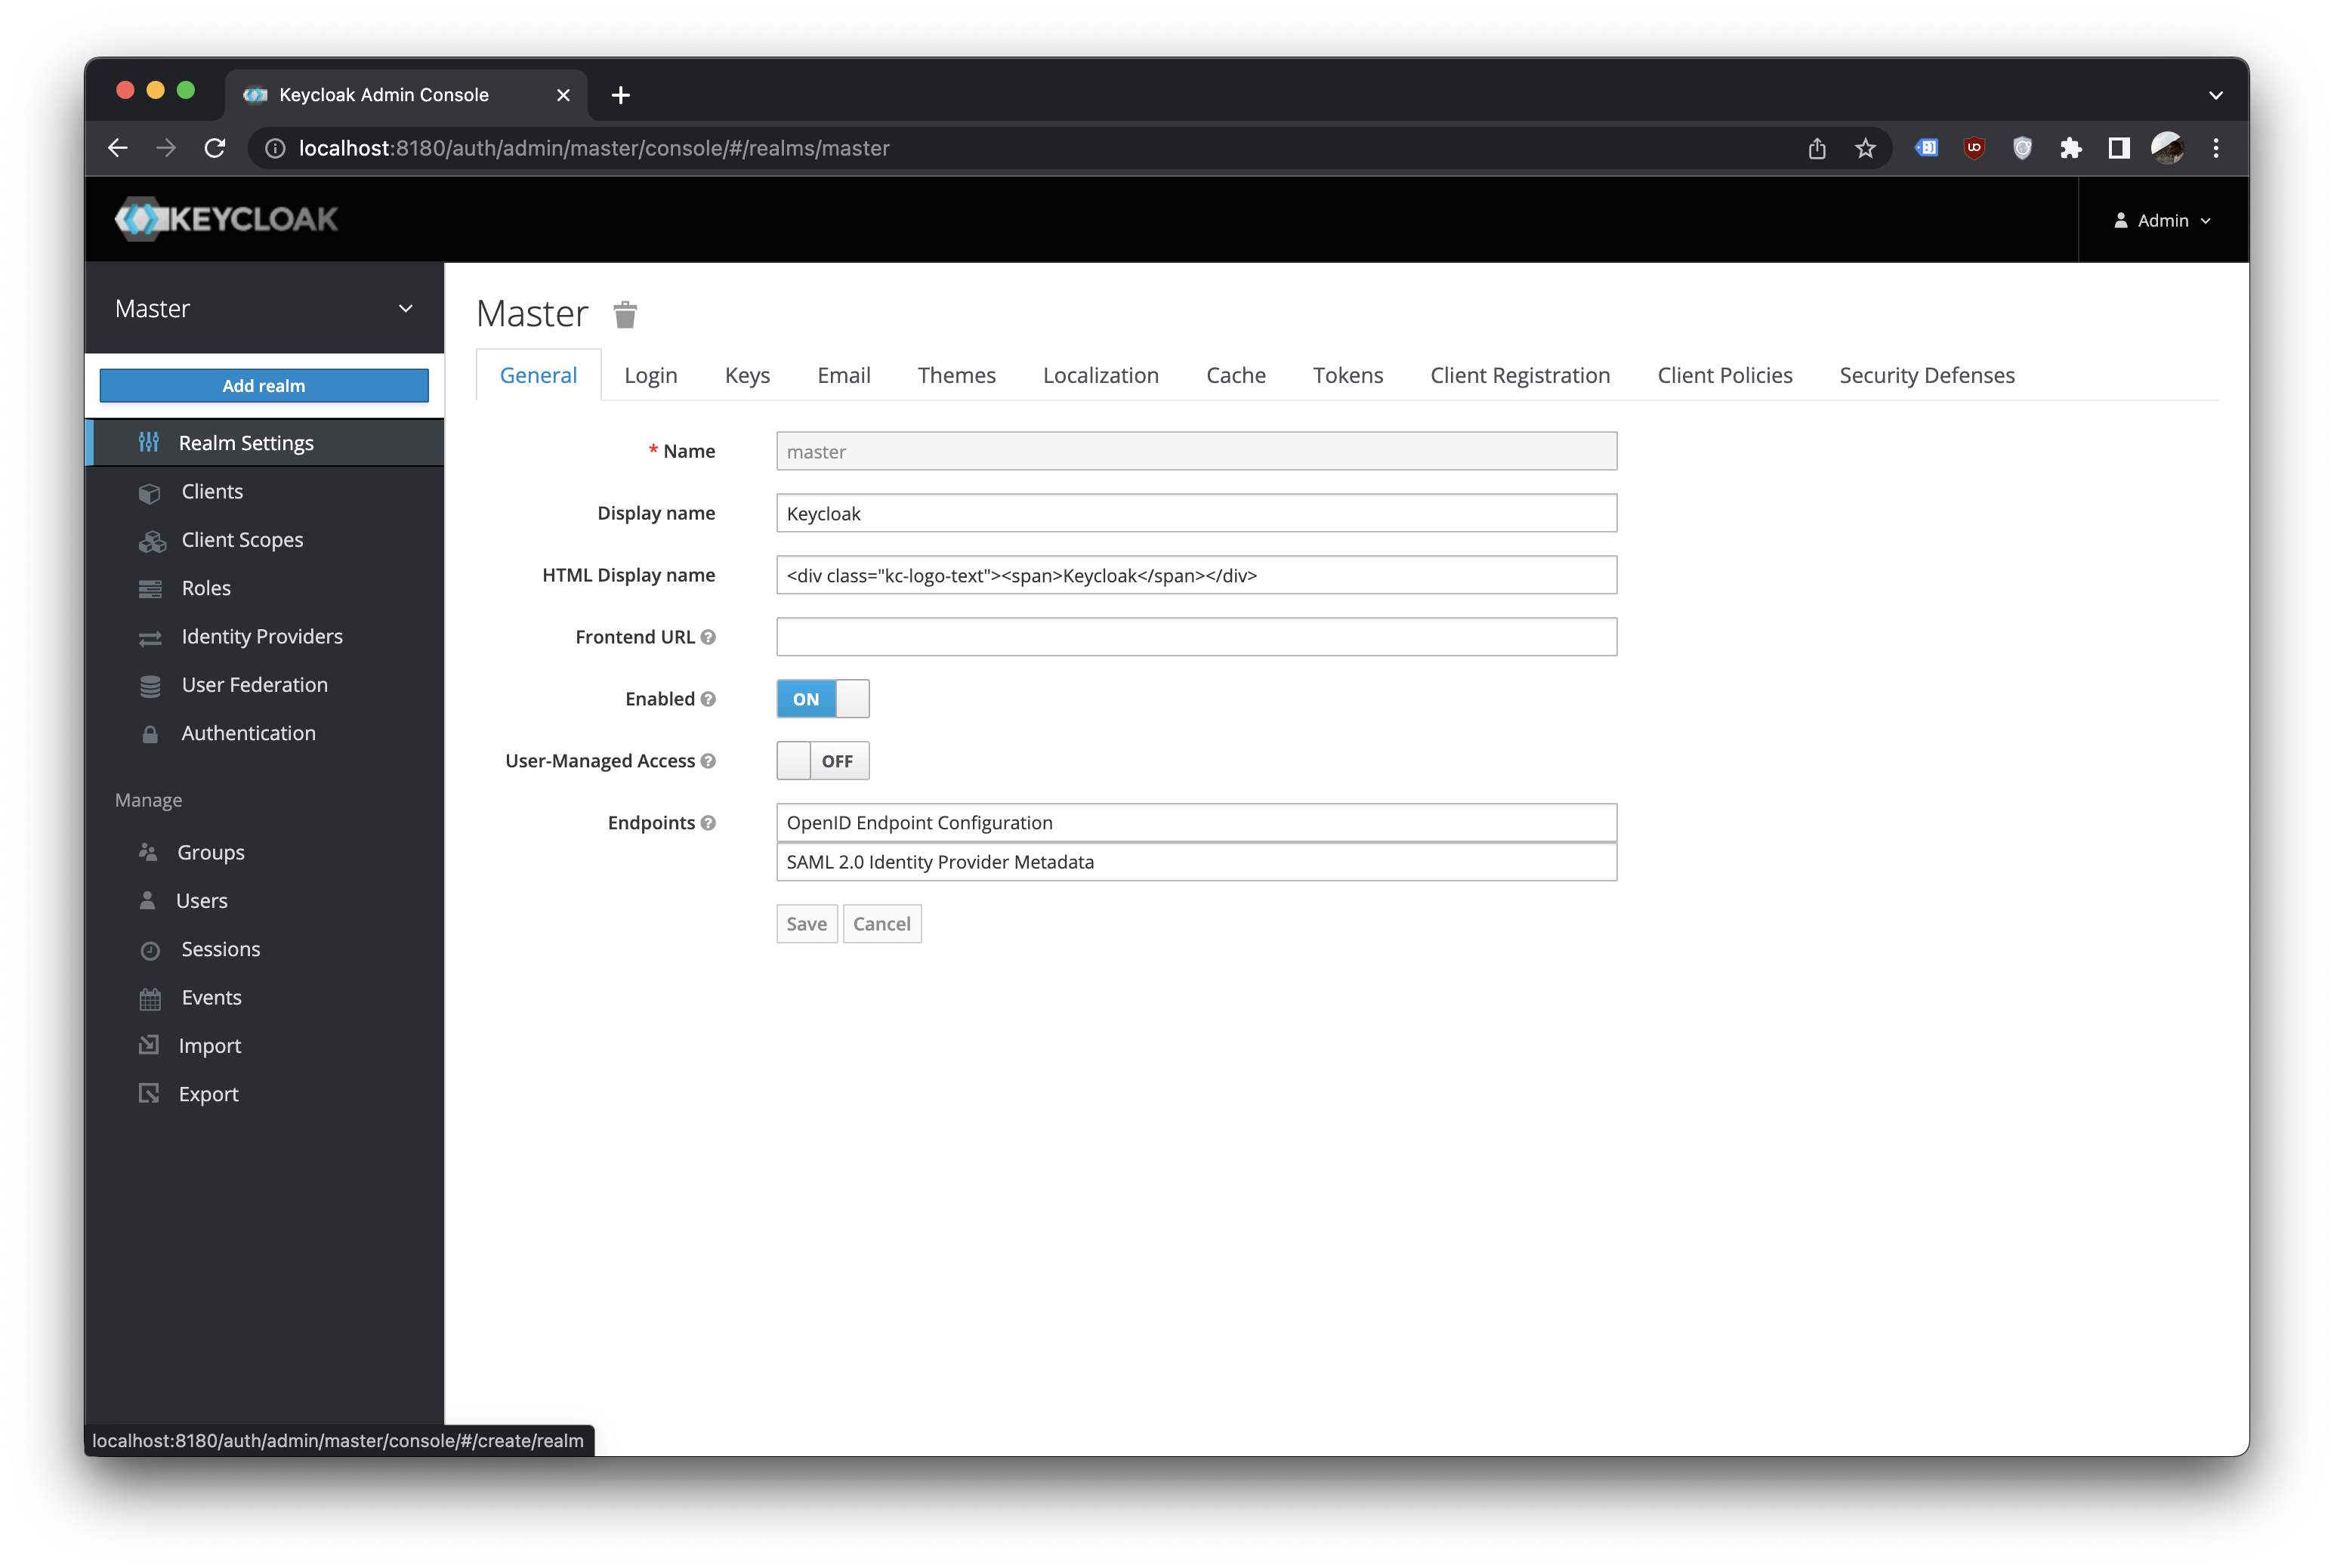
\includegraphics[width=0.80\linewidth]{keycloak_03.png}
\end{center}

Cliccando su \textit{Add realm} si aprirà un form che permetterà di iniziare a configurare il nostro realm

\textbf{Attenzione: da documentazione non è consigliato effettuare le configurazioni sul realm Master!}

\begin{center}
    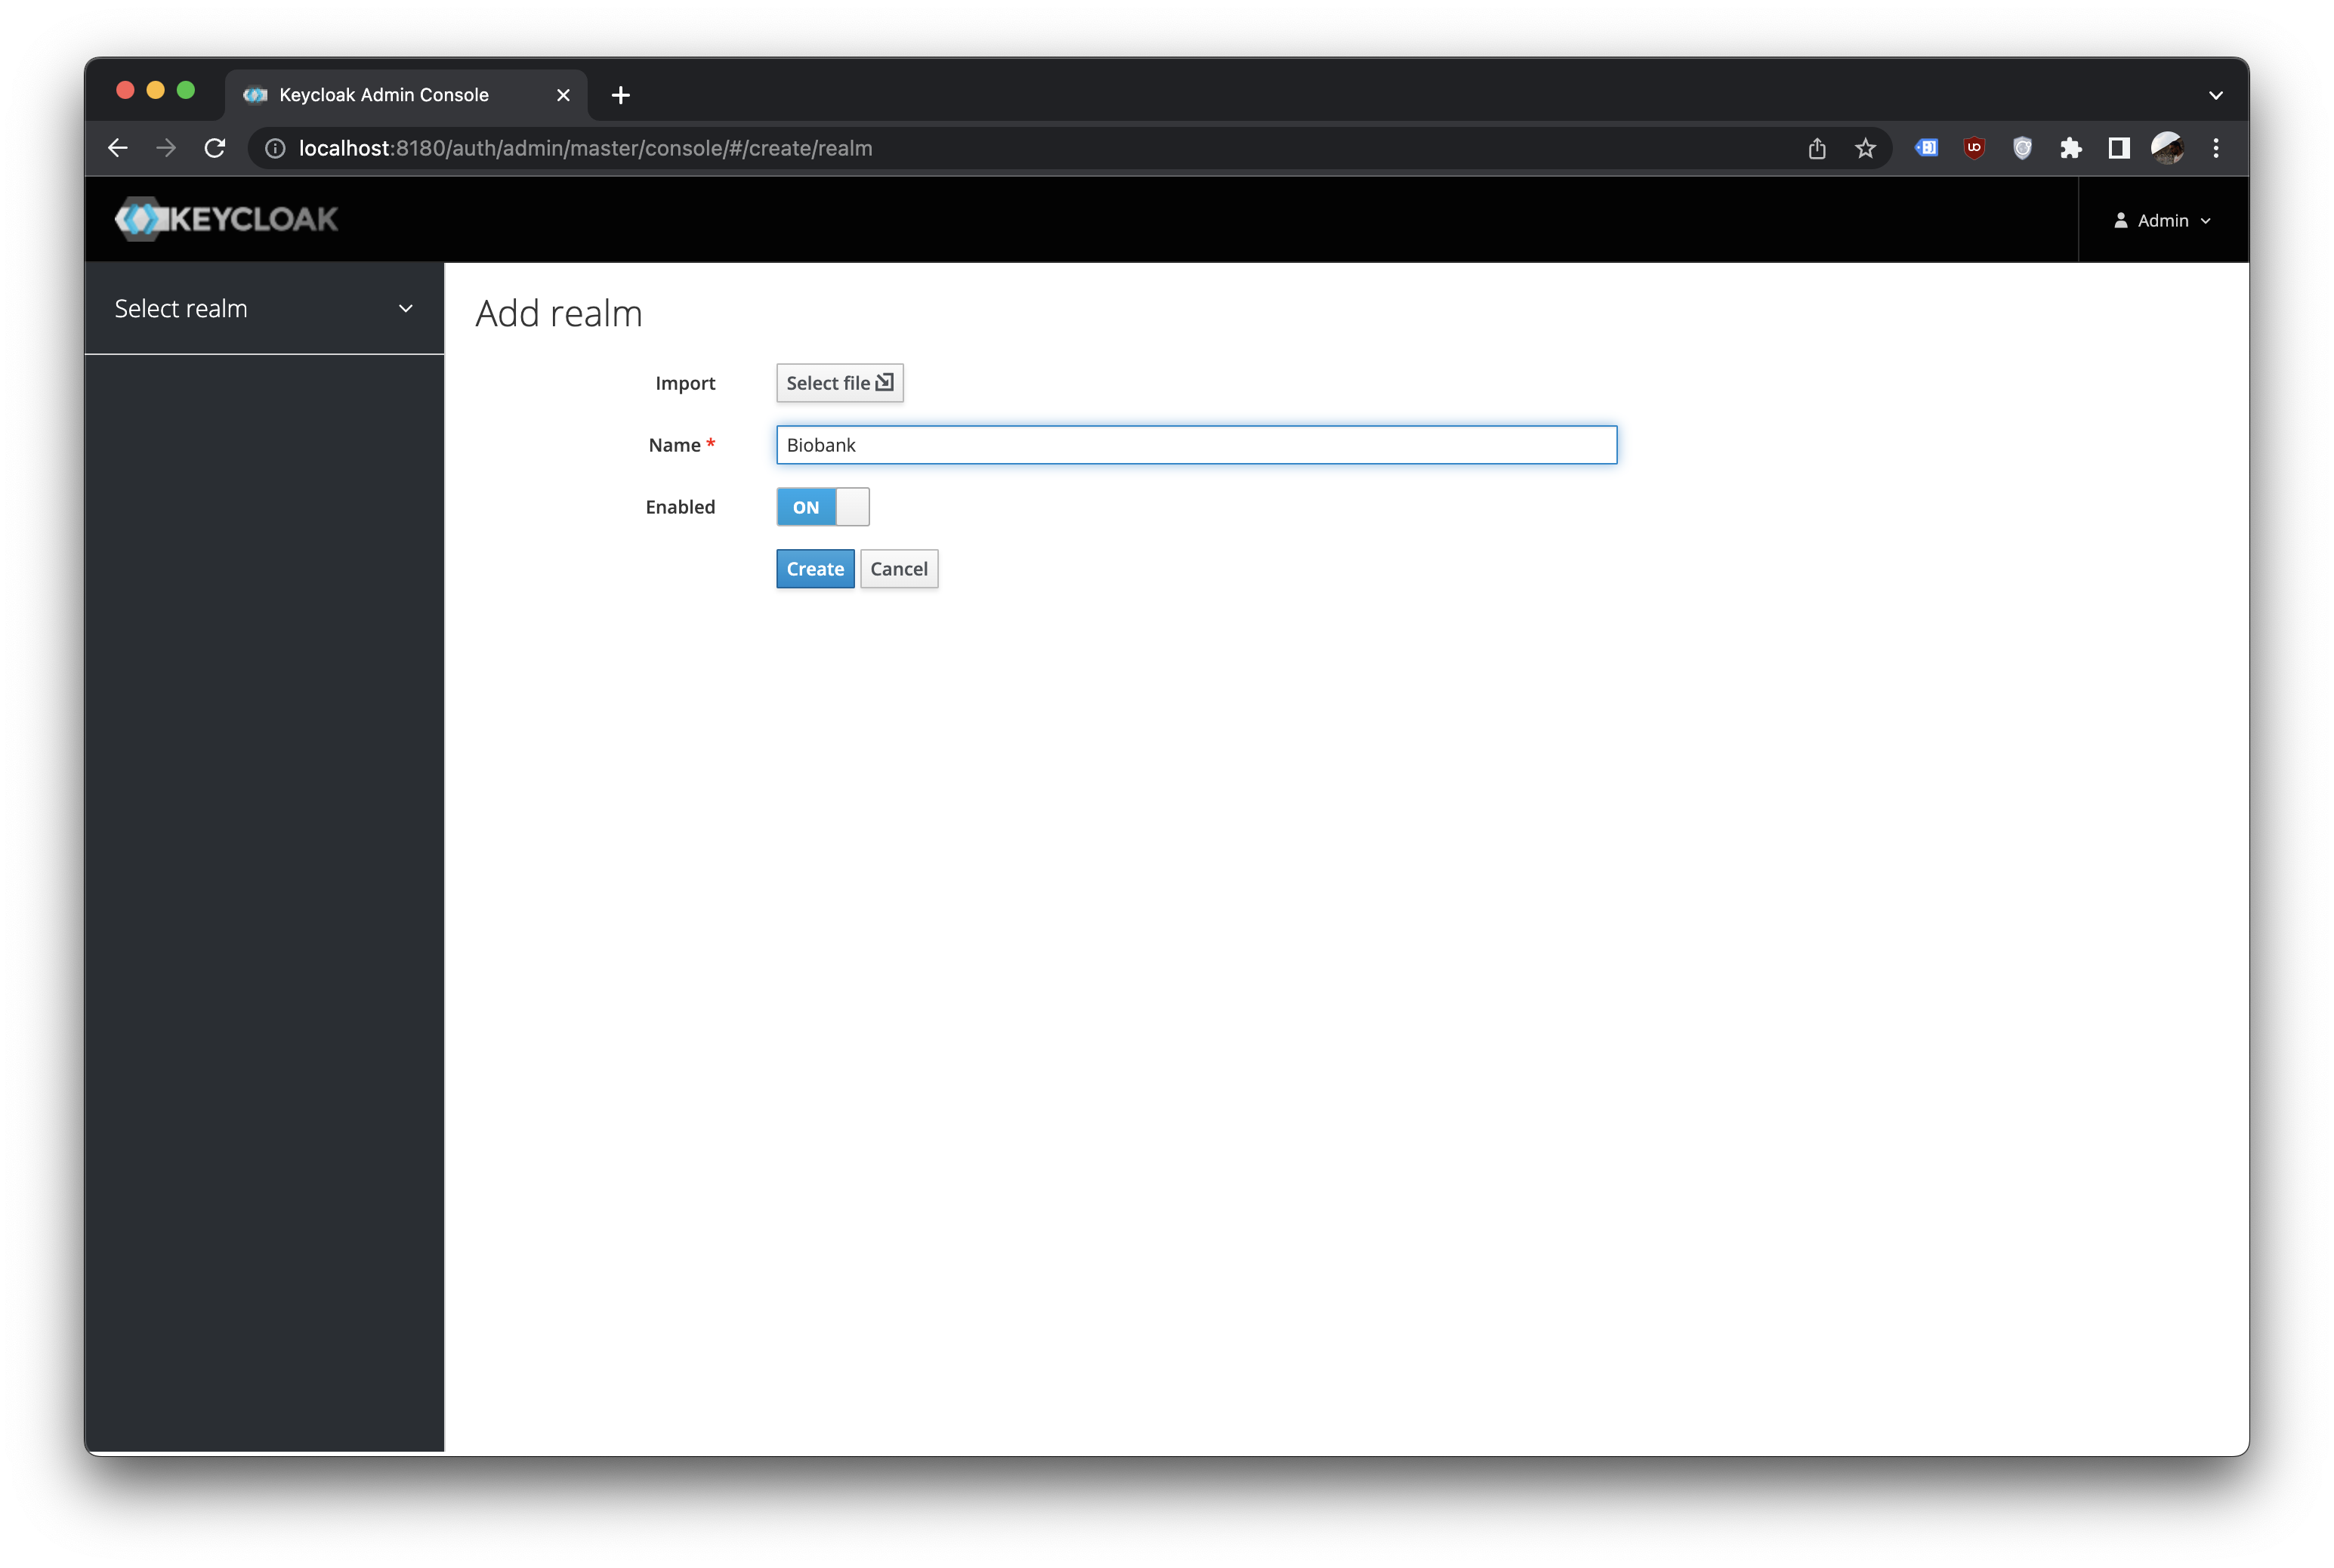
\includegraphics[width=0.80\linewidth]{keycloak_04.png}
\end{center}

Vi è anche l'opzione di importare i settings del realm da file \texttt{.json}

\textbf{NB: I nomi assegnati sono tutti case sensitive!}

\subsection{Creazione di un client}

Una volta creato il realm, dirigiamoci sul tab \textit{Clients} e clicchiamo sul pulsante \textit{Create}

\begin{center}
    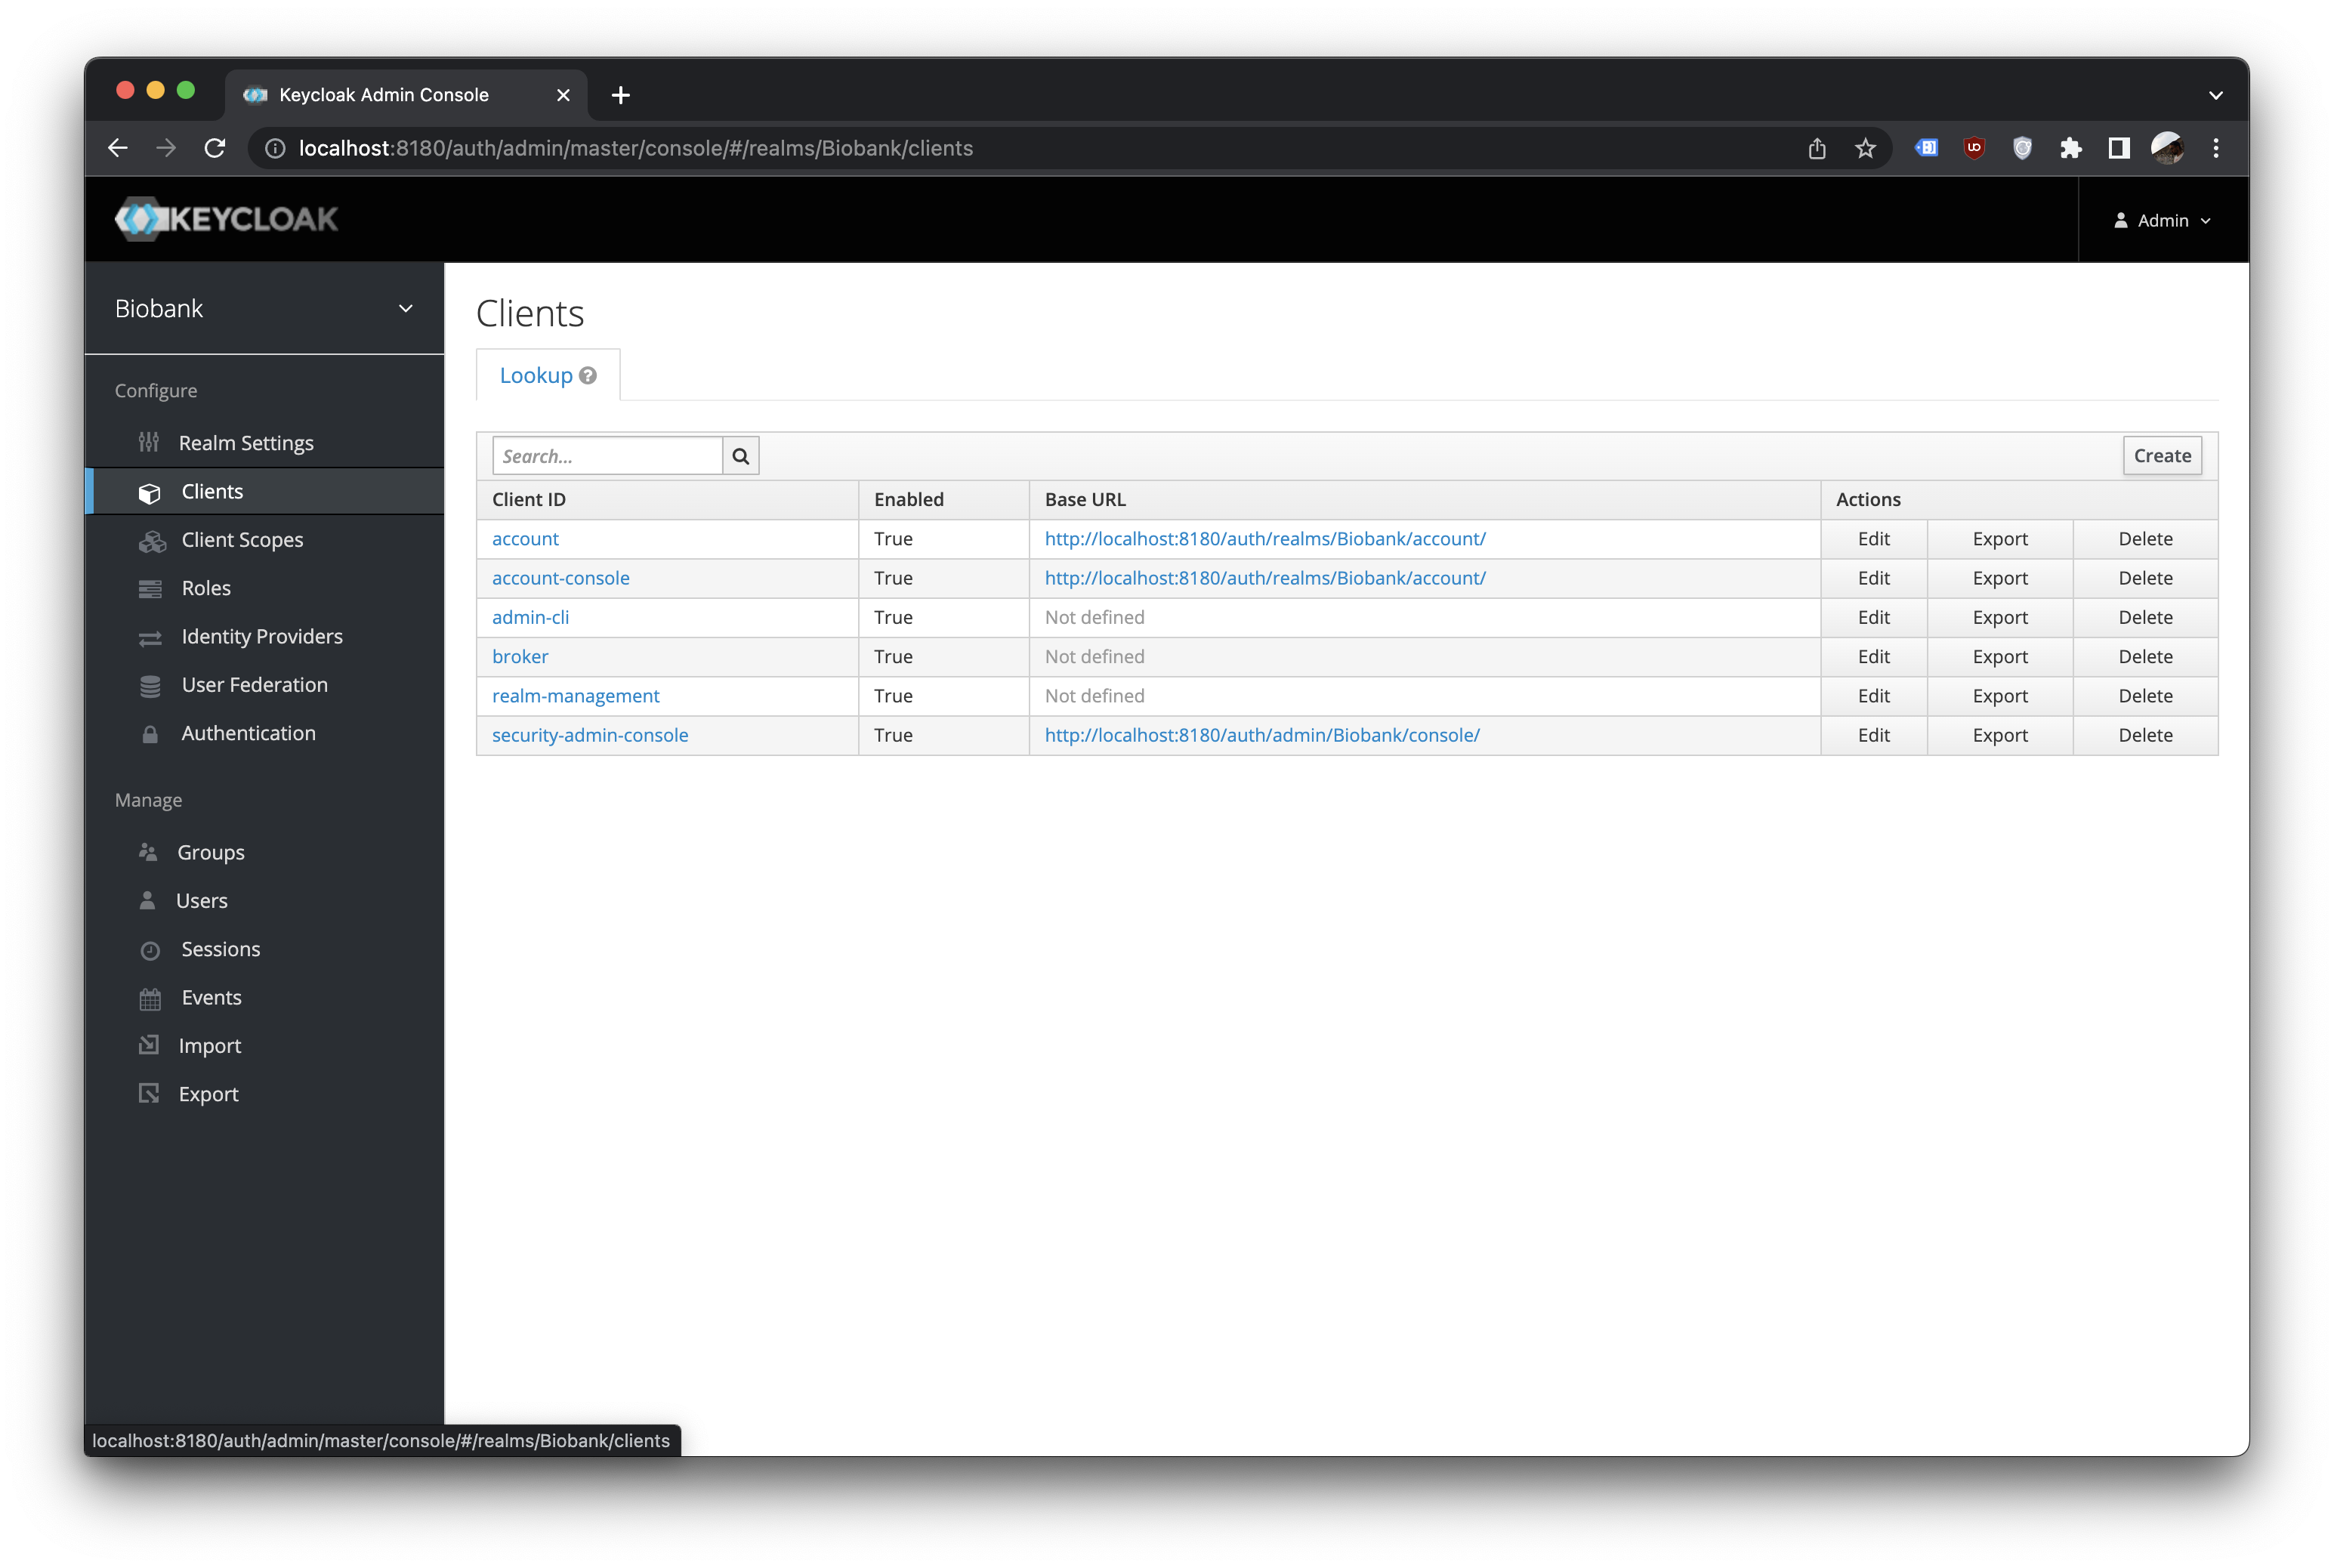
\includegraphics[width=0.80\linewidth]{keycloak_05.png}
\end{center}

Inseriamo il nostro client id e clicchiamo su \textit{Save}

\begin{center}
    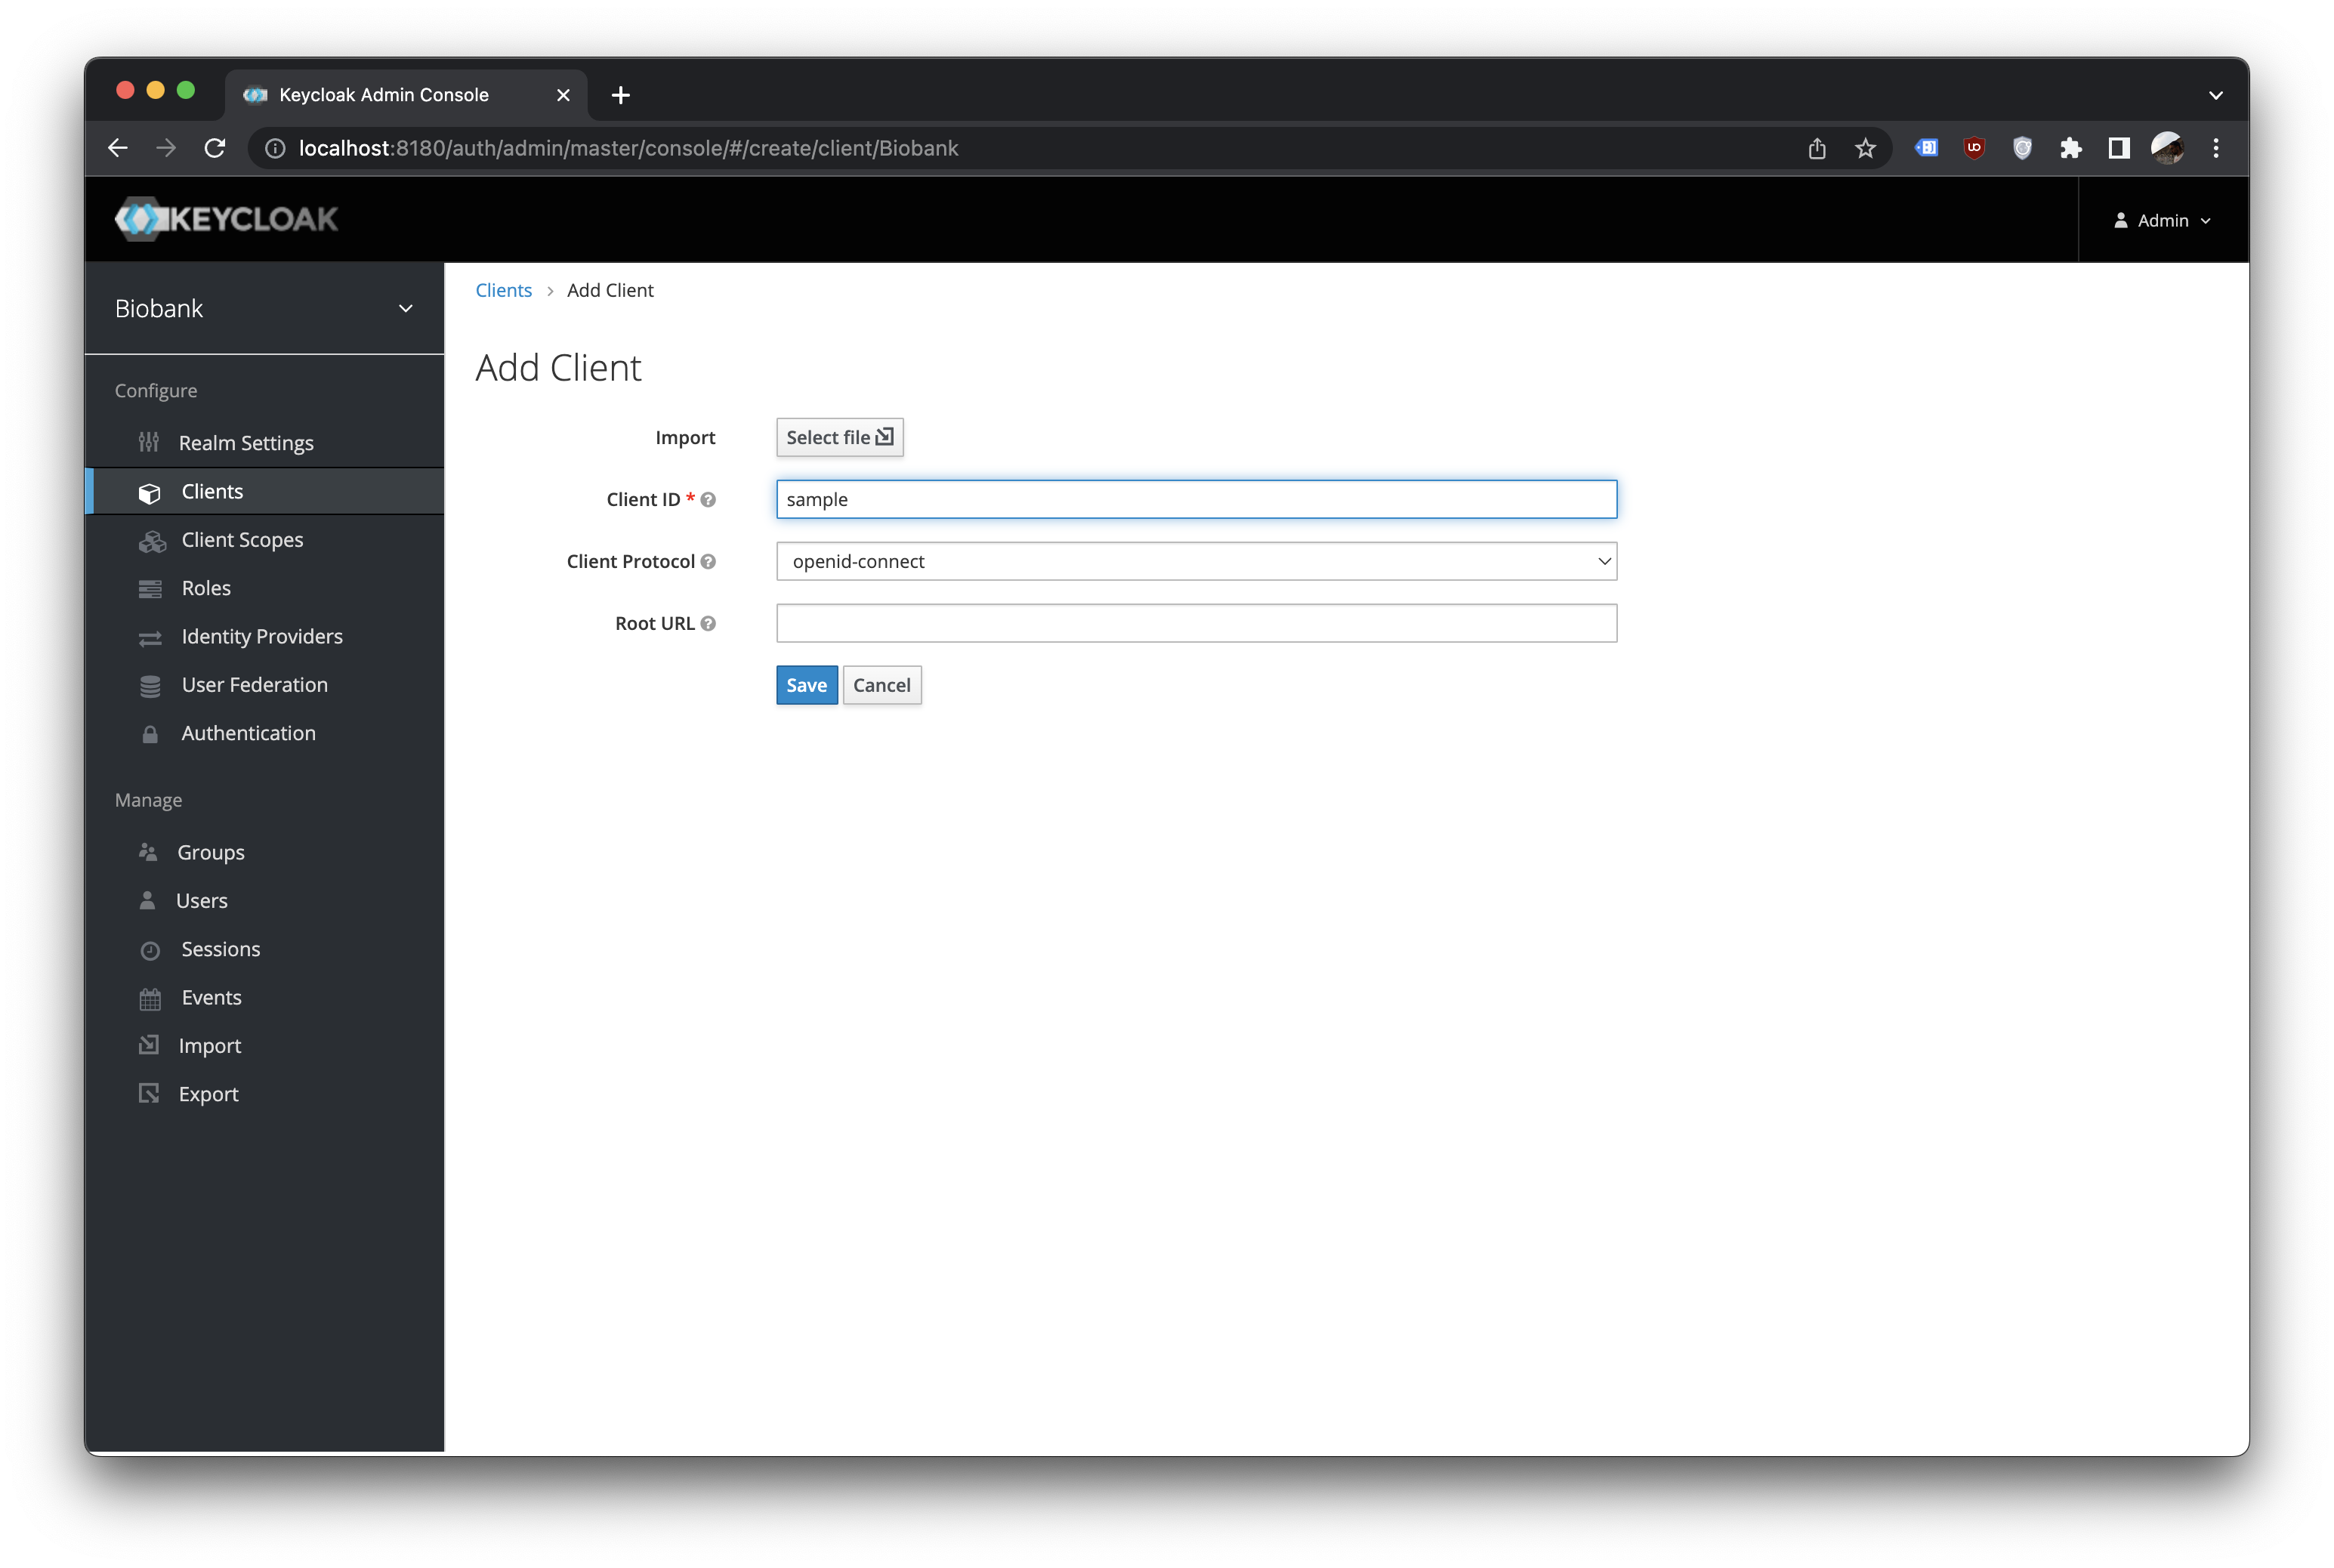
\includegraphics[width=0.80\linewidth]{keycloak_06.png}
\end{center}

Dopo aver salvato le configurazioni del nuovo client la pagina si aggiornerà con nuovi campi. Per prima cosa è necessario
assegnare uno o più \textit{Valid redirect URIs} (cioé, un elenco di URI validi sui quali il browser può reindirizzare dopo login o logout), nel nostro caso inseriamo l'indirizzo del nostro microservizio.

\begin{center}
    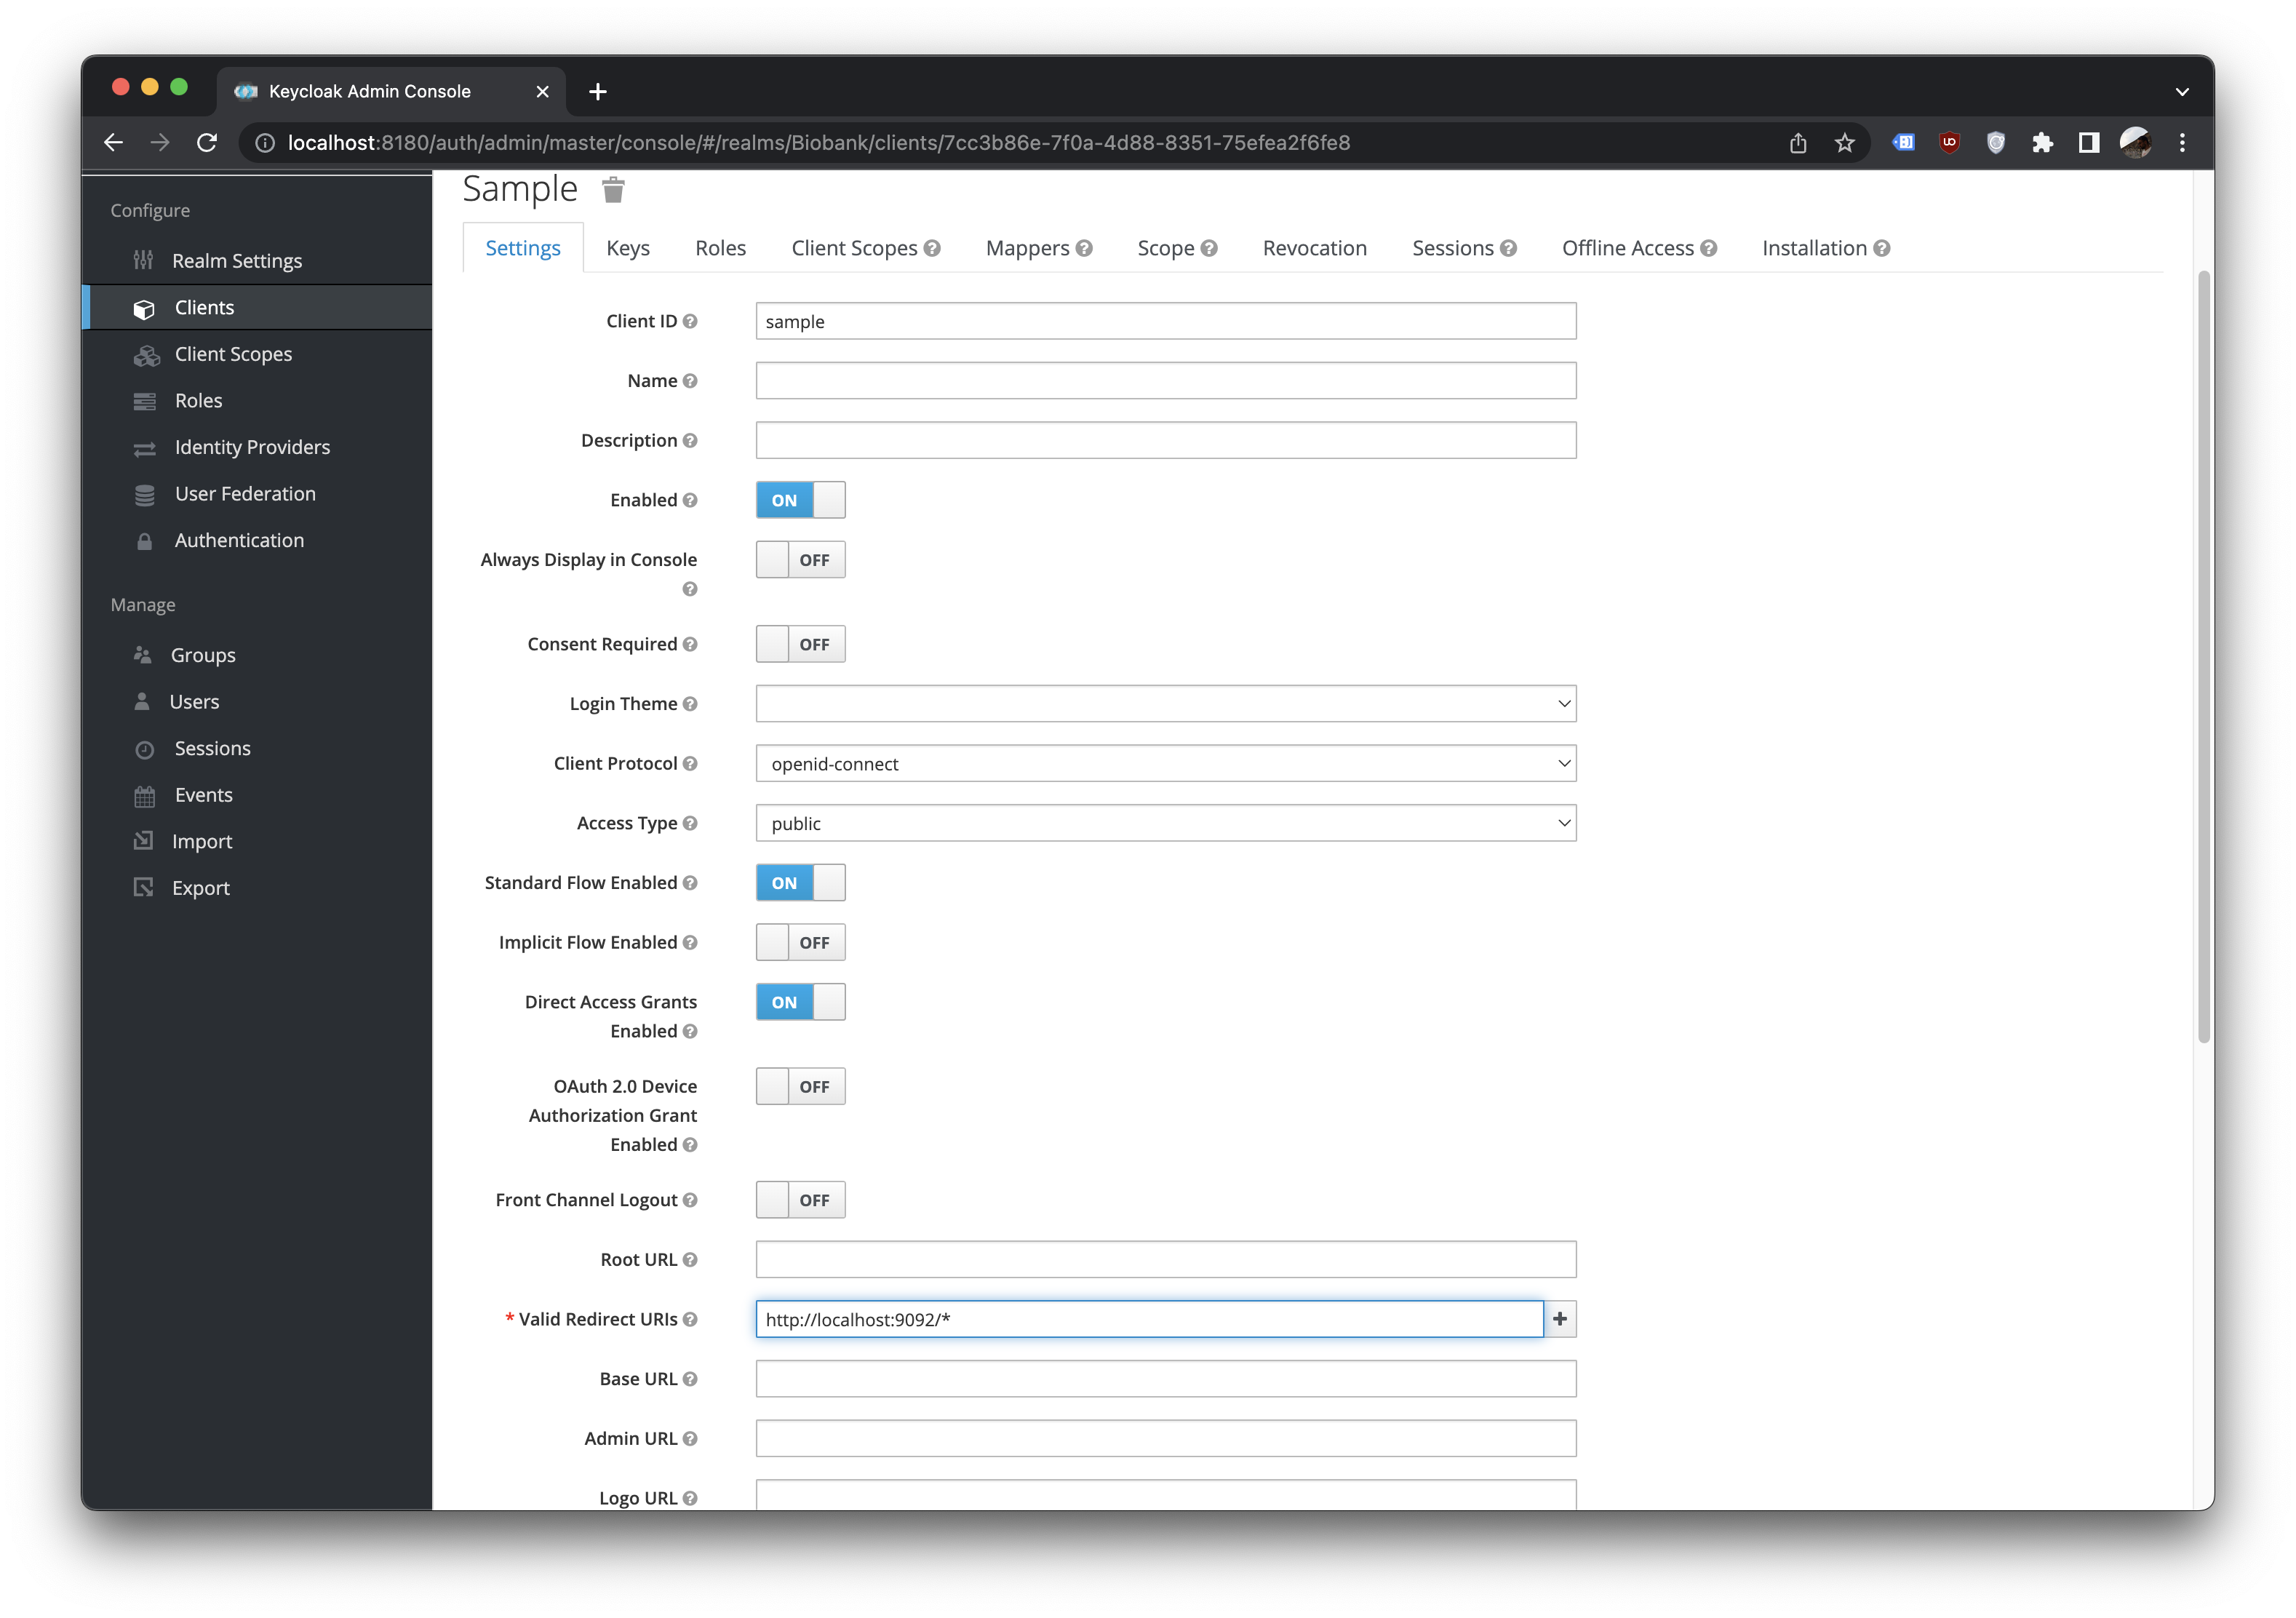
\includegraphics[width=0.80\linewidth]{keycloak_07.png}
\end{center}

\subsection{Creazione di un ruolo}

Infine, cliccare sulla tab in alto \textit{Roles}.

\begin{center}
    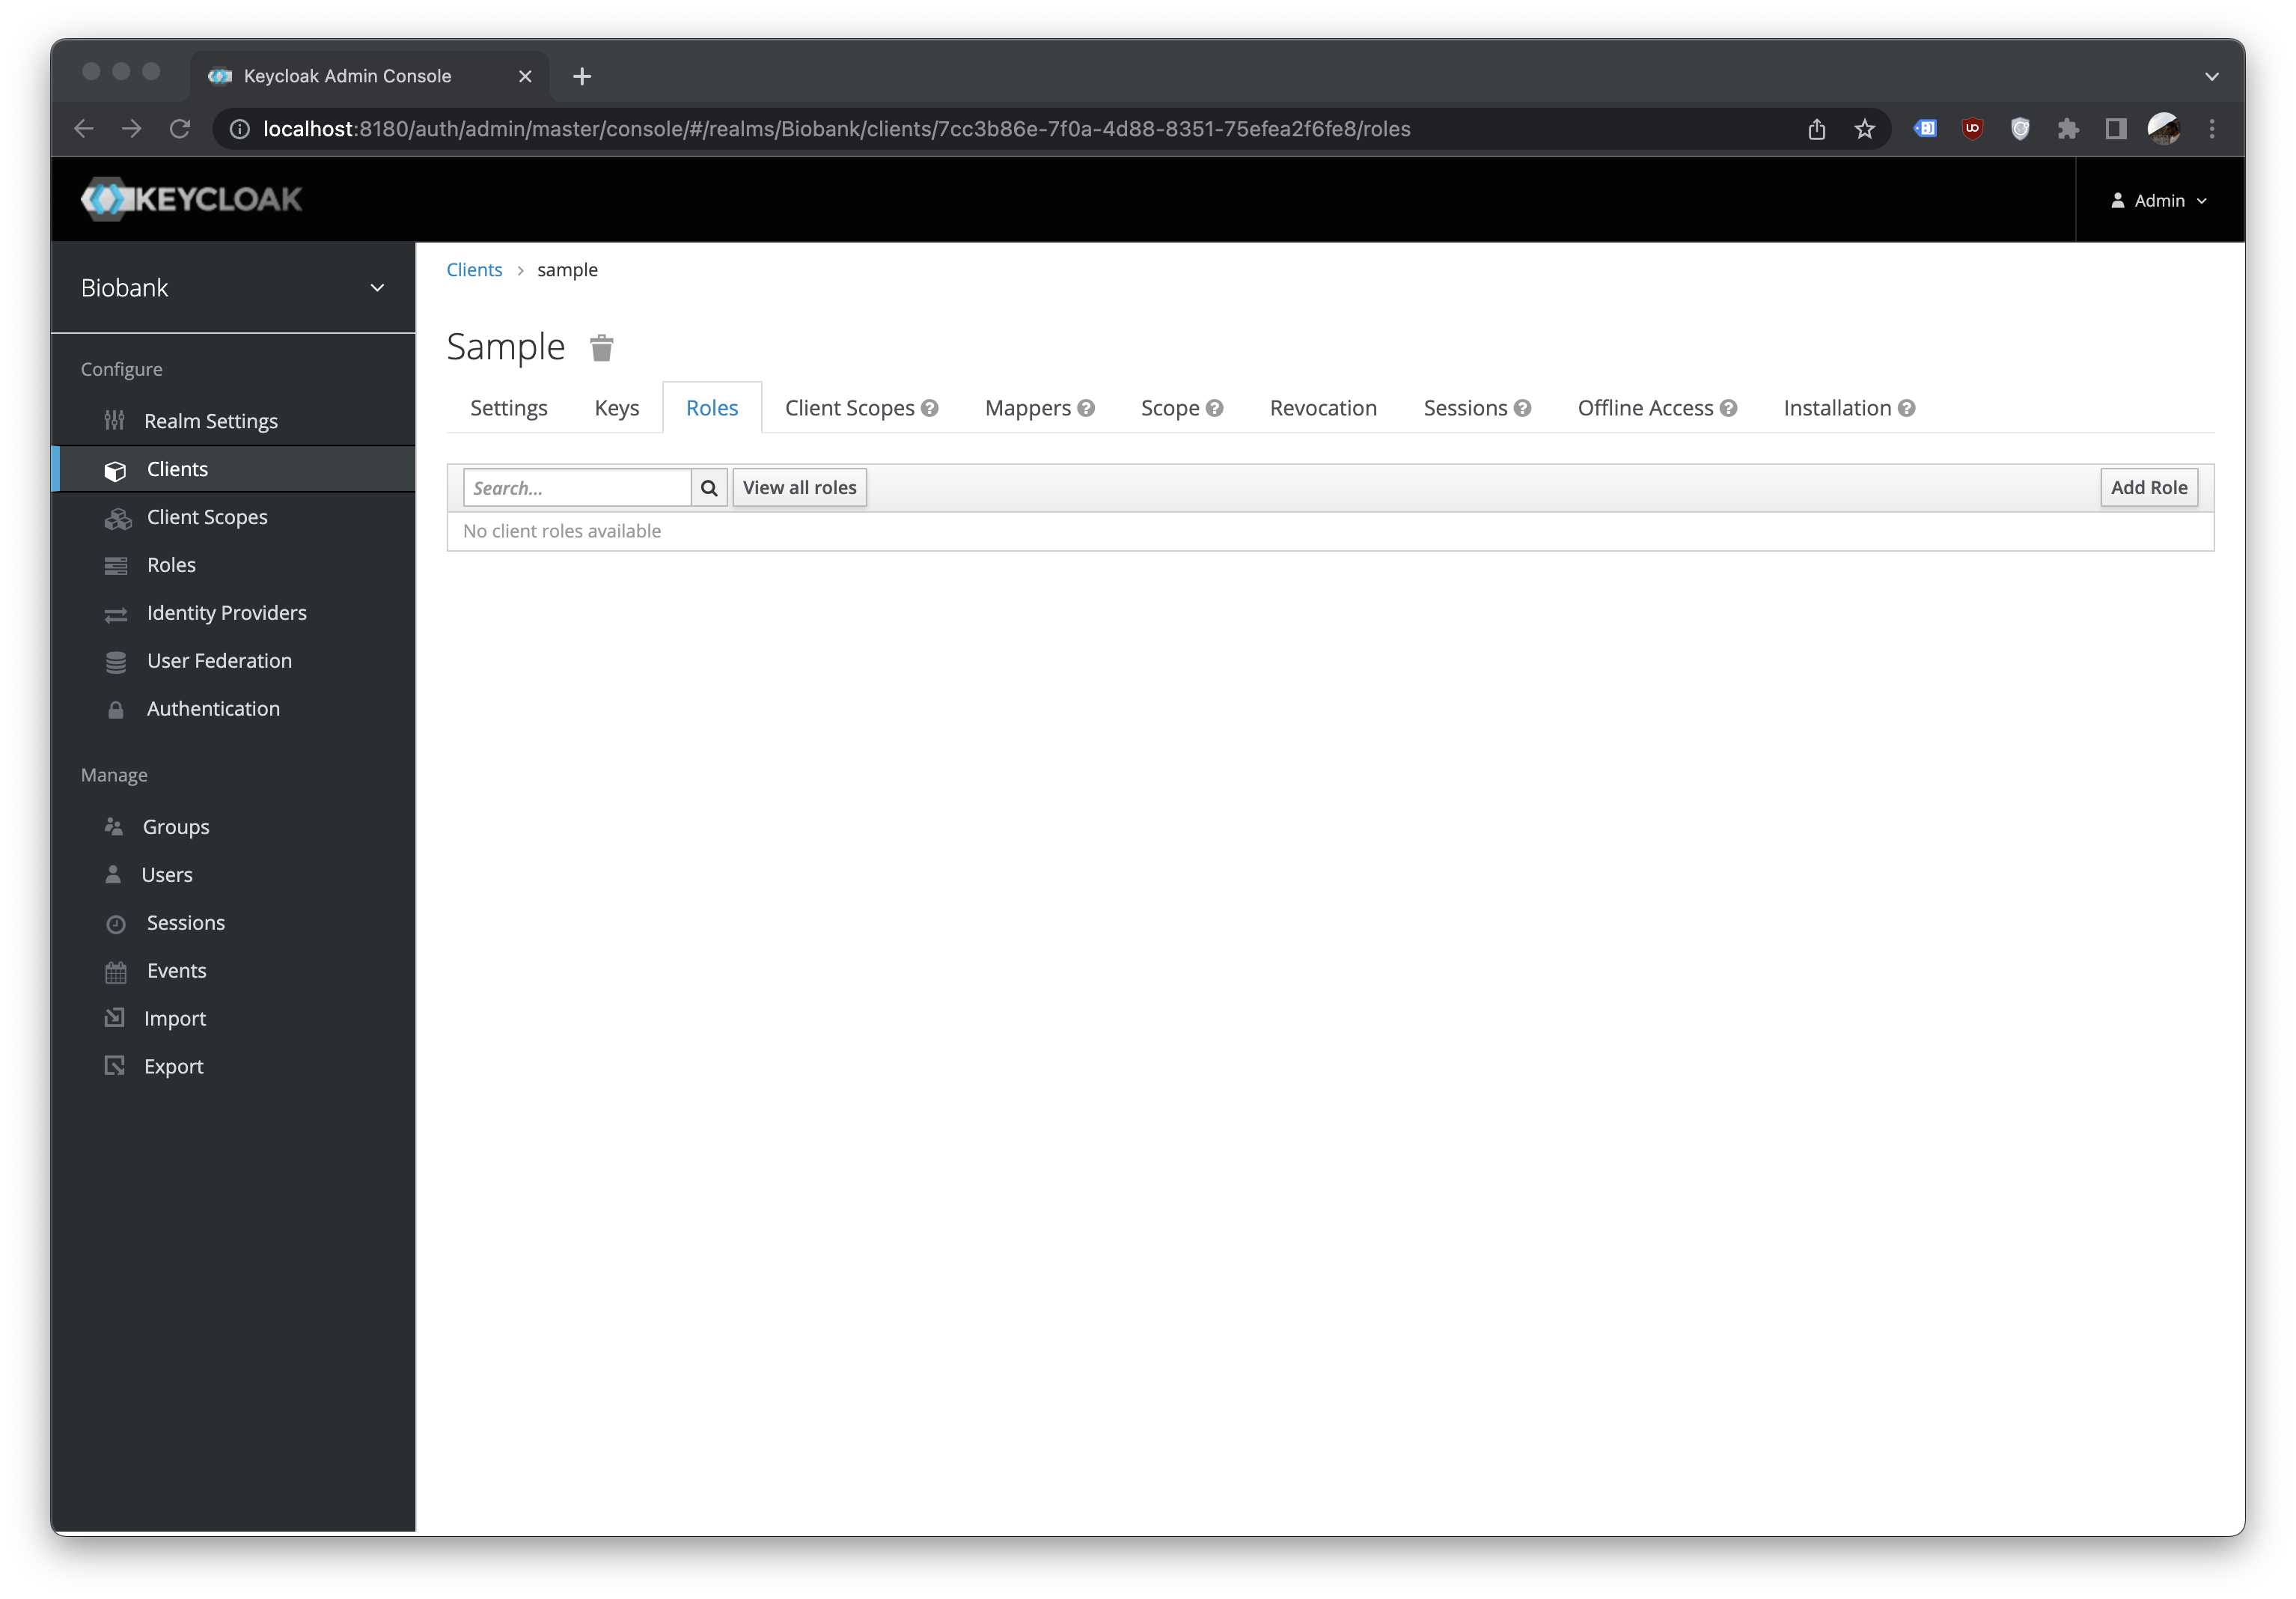
\includegraphics[width=0.80\linewidth]{keycloak_08.png}
\end{center}

Si nota che la lista di ruoli è vuota, cliccare su \textit{Add Role}.

\begin{center}
    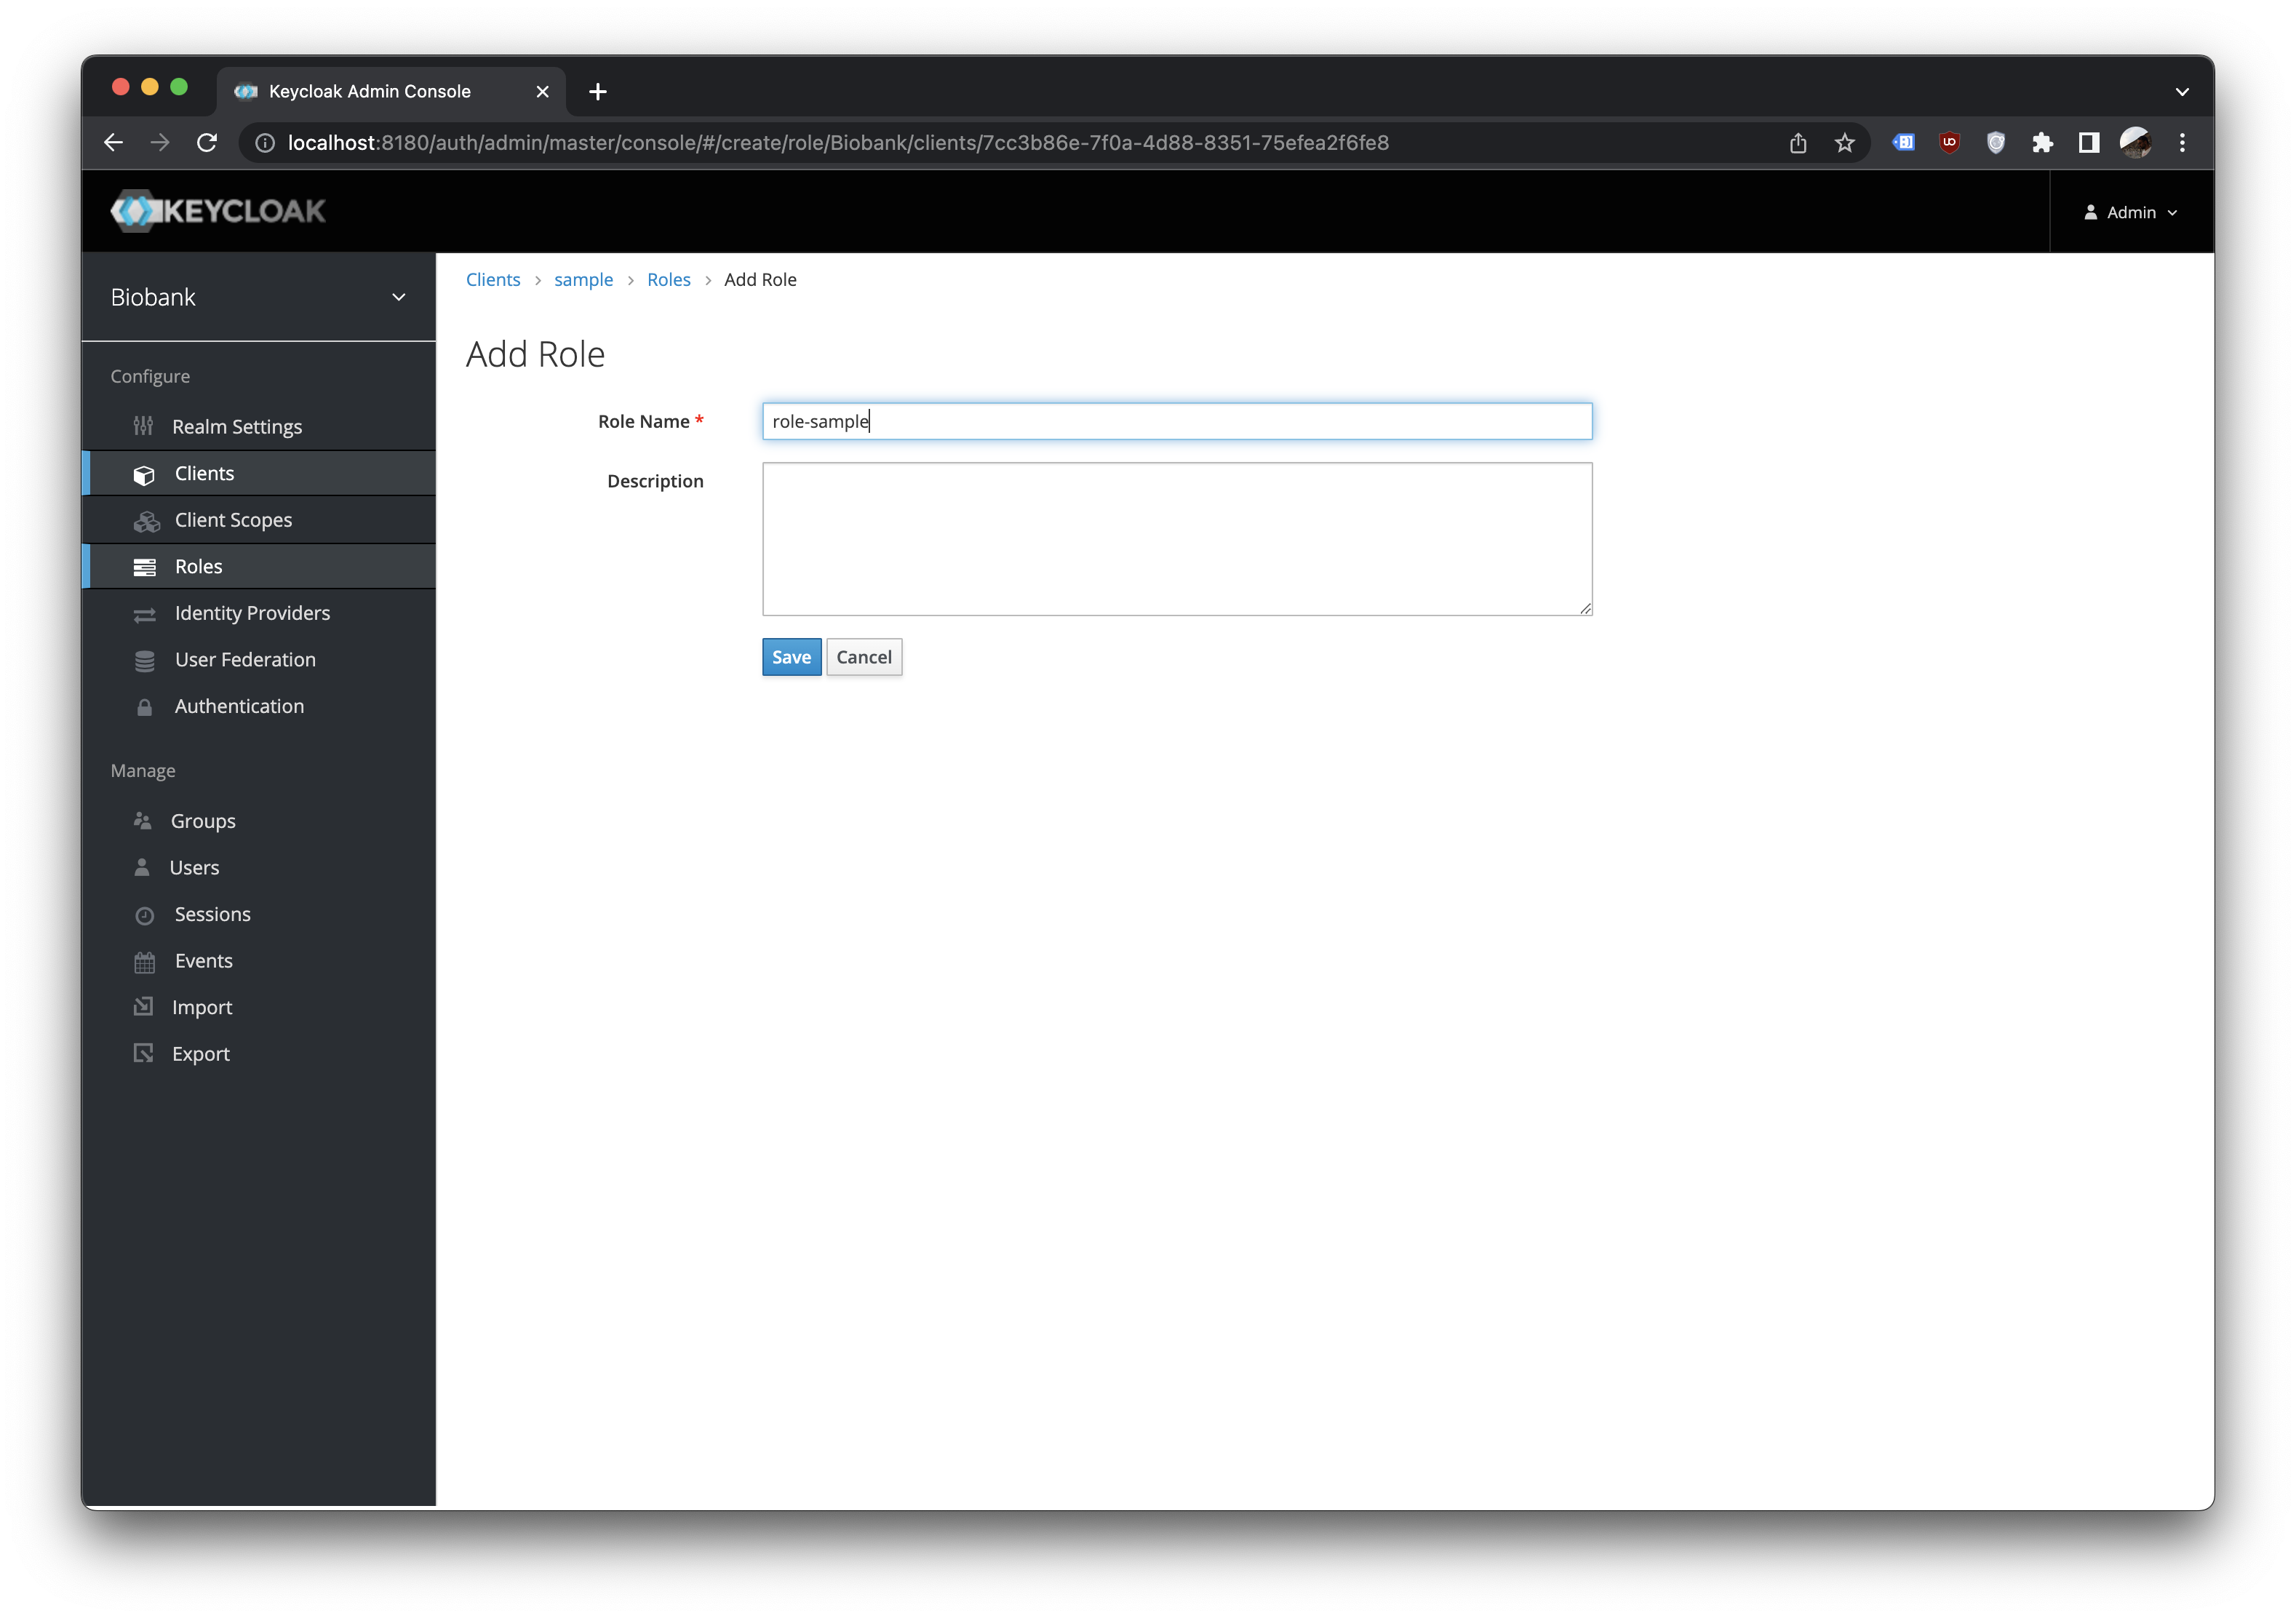
\includegraphics[width=0.80\linewidth]{keycloak_09.png}
\end{center}

Dopo aver scelto il nome del ruolo cliccare su \textit{Save}. Tornando indietro, al tab \textit{Roles} del client precedentemente selezionato, il nostro ruolo apparirà nella lista.

\begin{center}
    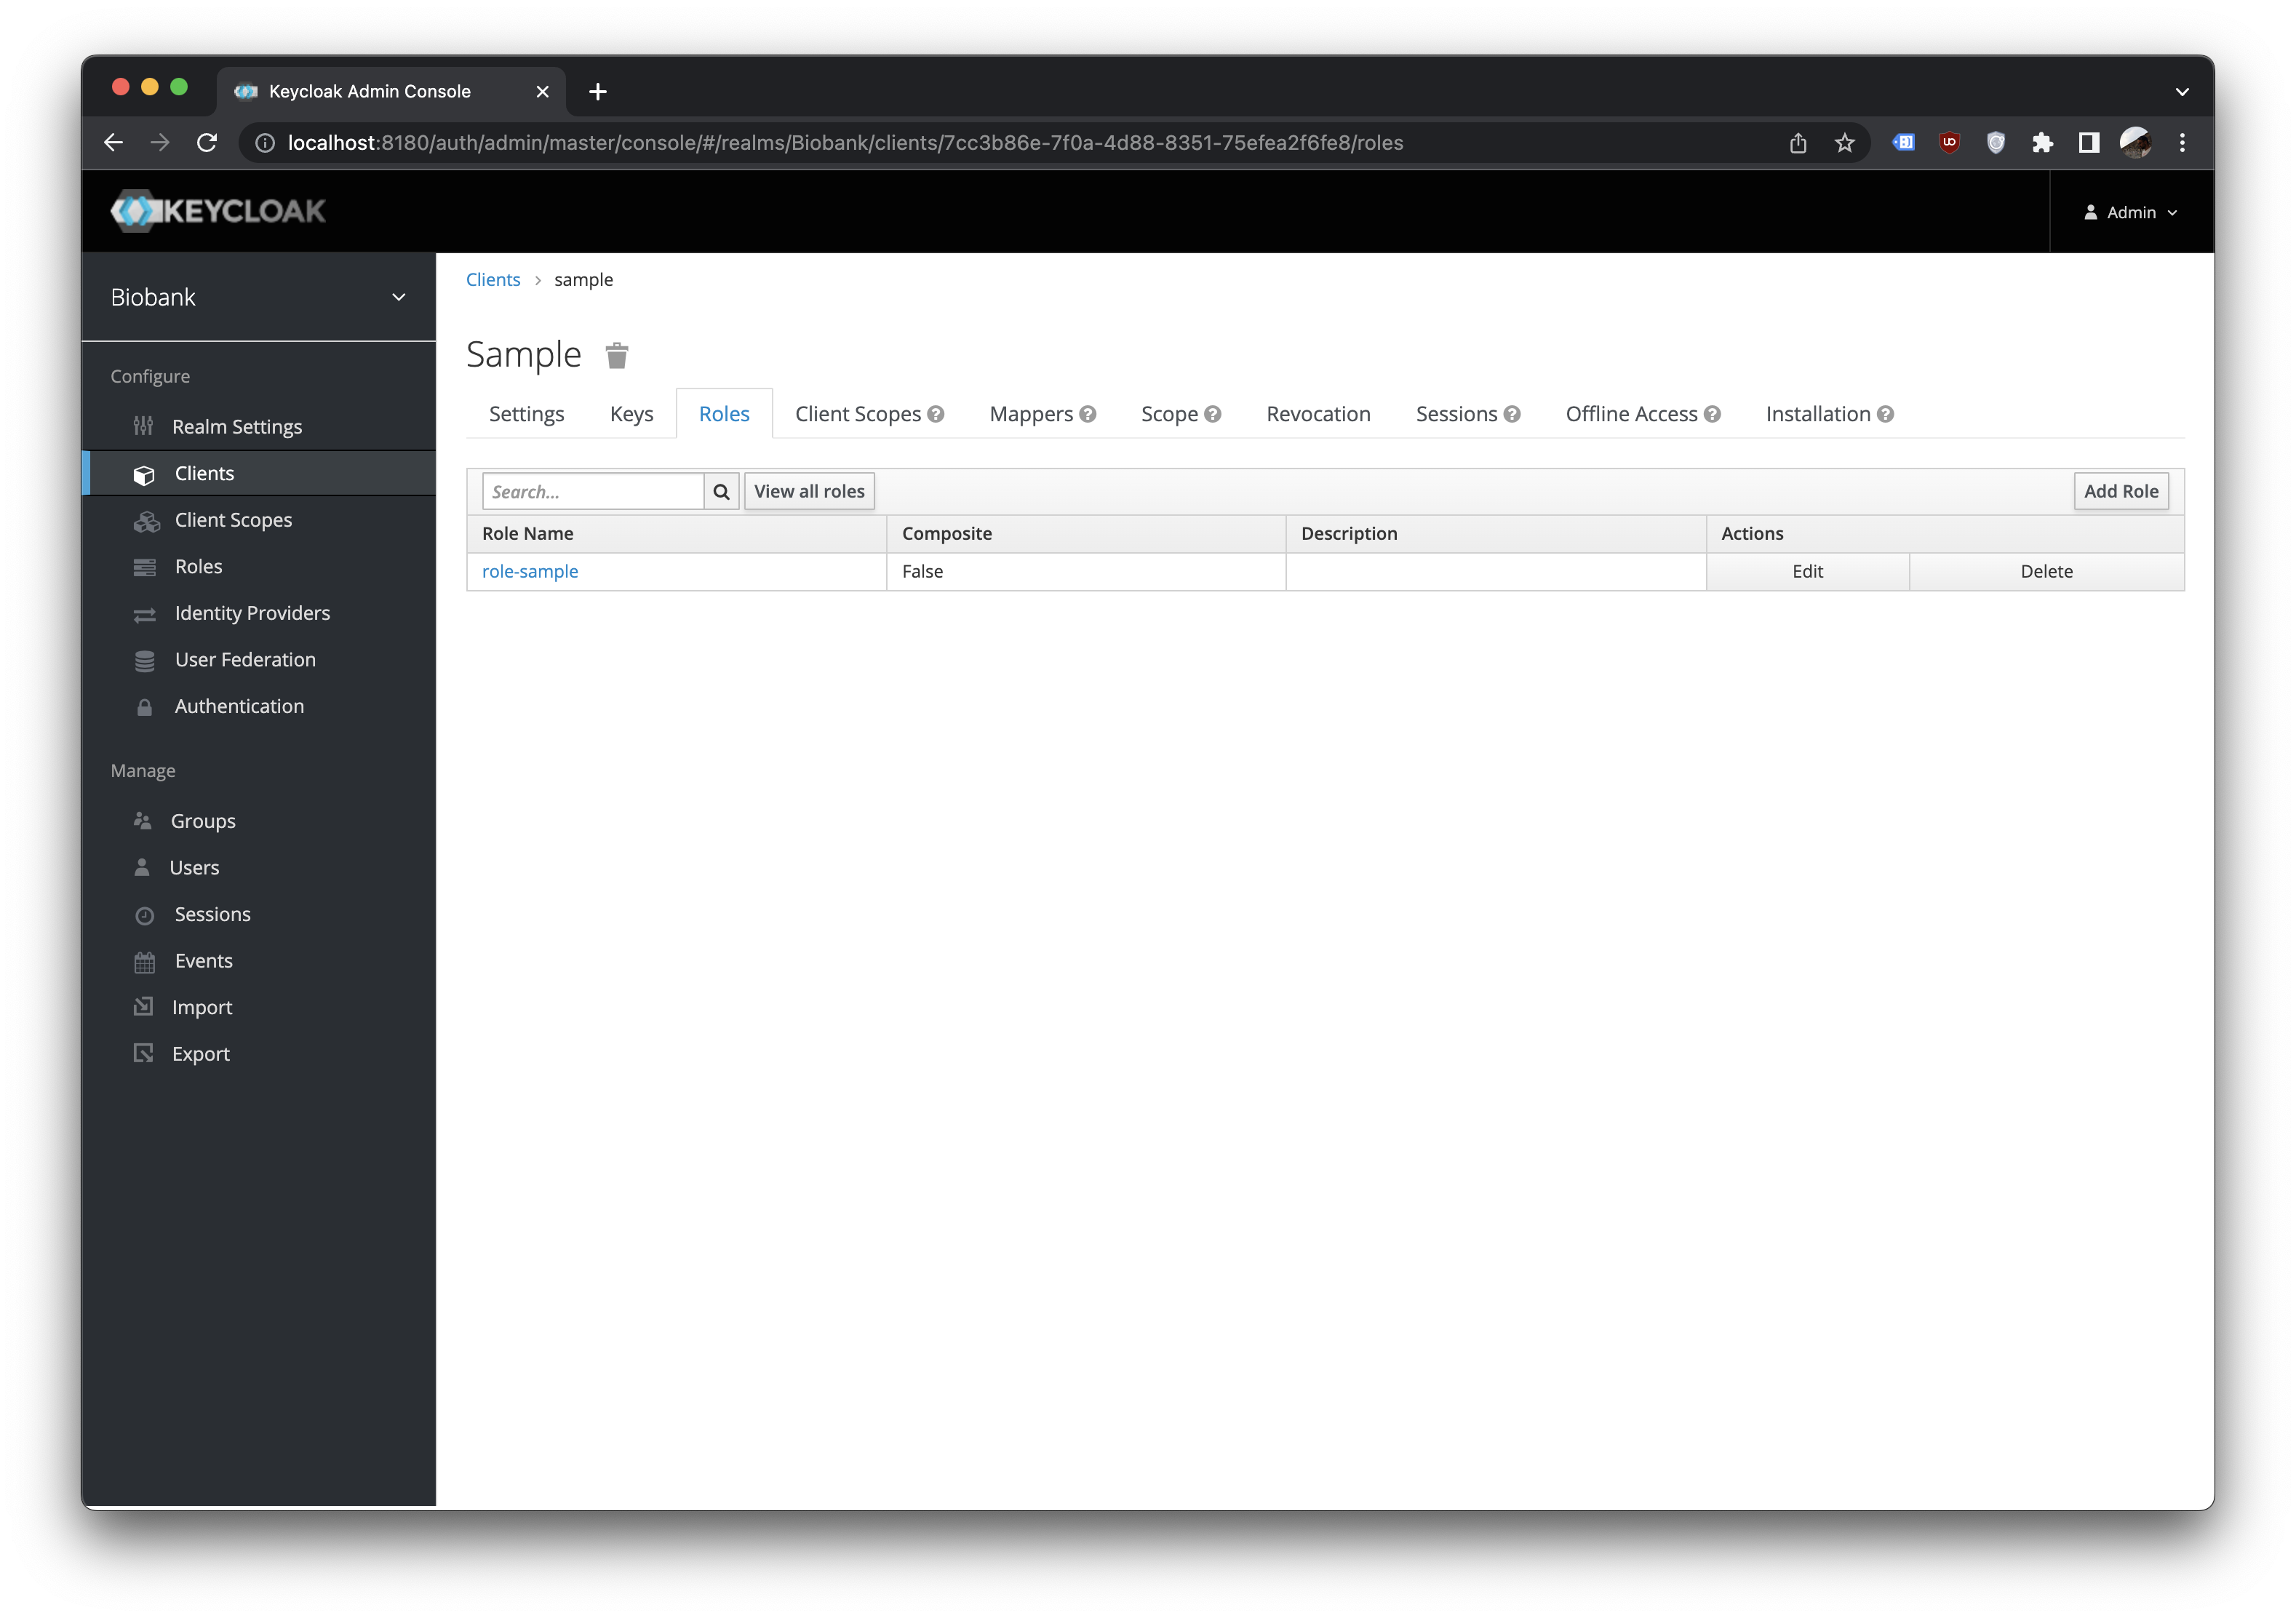
\includegraphics[width=0.80\linewidth]{keycloak_10.png}
\end{center}

\subsection{Creazione di un utente ed assegnazione di un ruolo}

Si nota che Keycloak fornisce le pagine di login e registrazione degli utenti (personalizzabili).
Tuttavia, in questo caso, si prenderà in esame solo la parte di \textit{gestione} dell'utenza lato back-office. Per eventuali guardare le reference a fine elaborato.
Clicchiamo dunque sul tab della sidebar di sinistra su \textit{Users}.

\begin{center}
    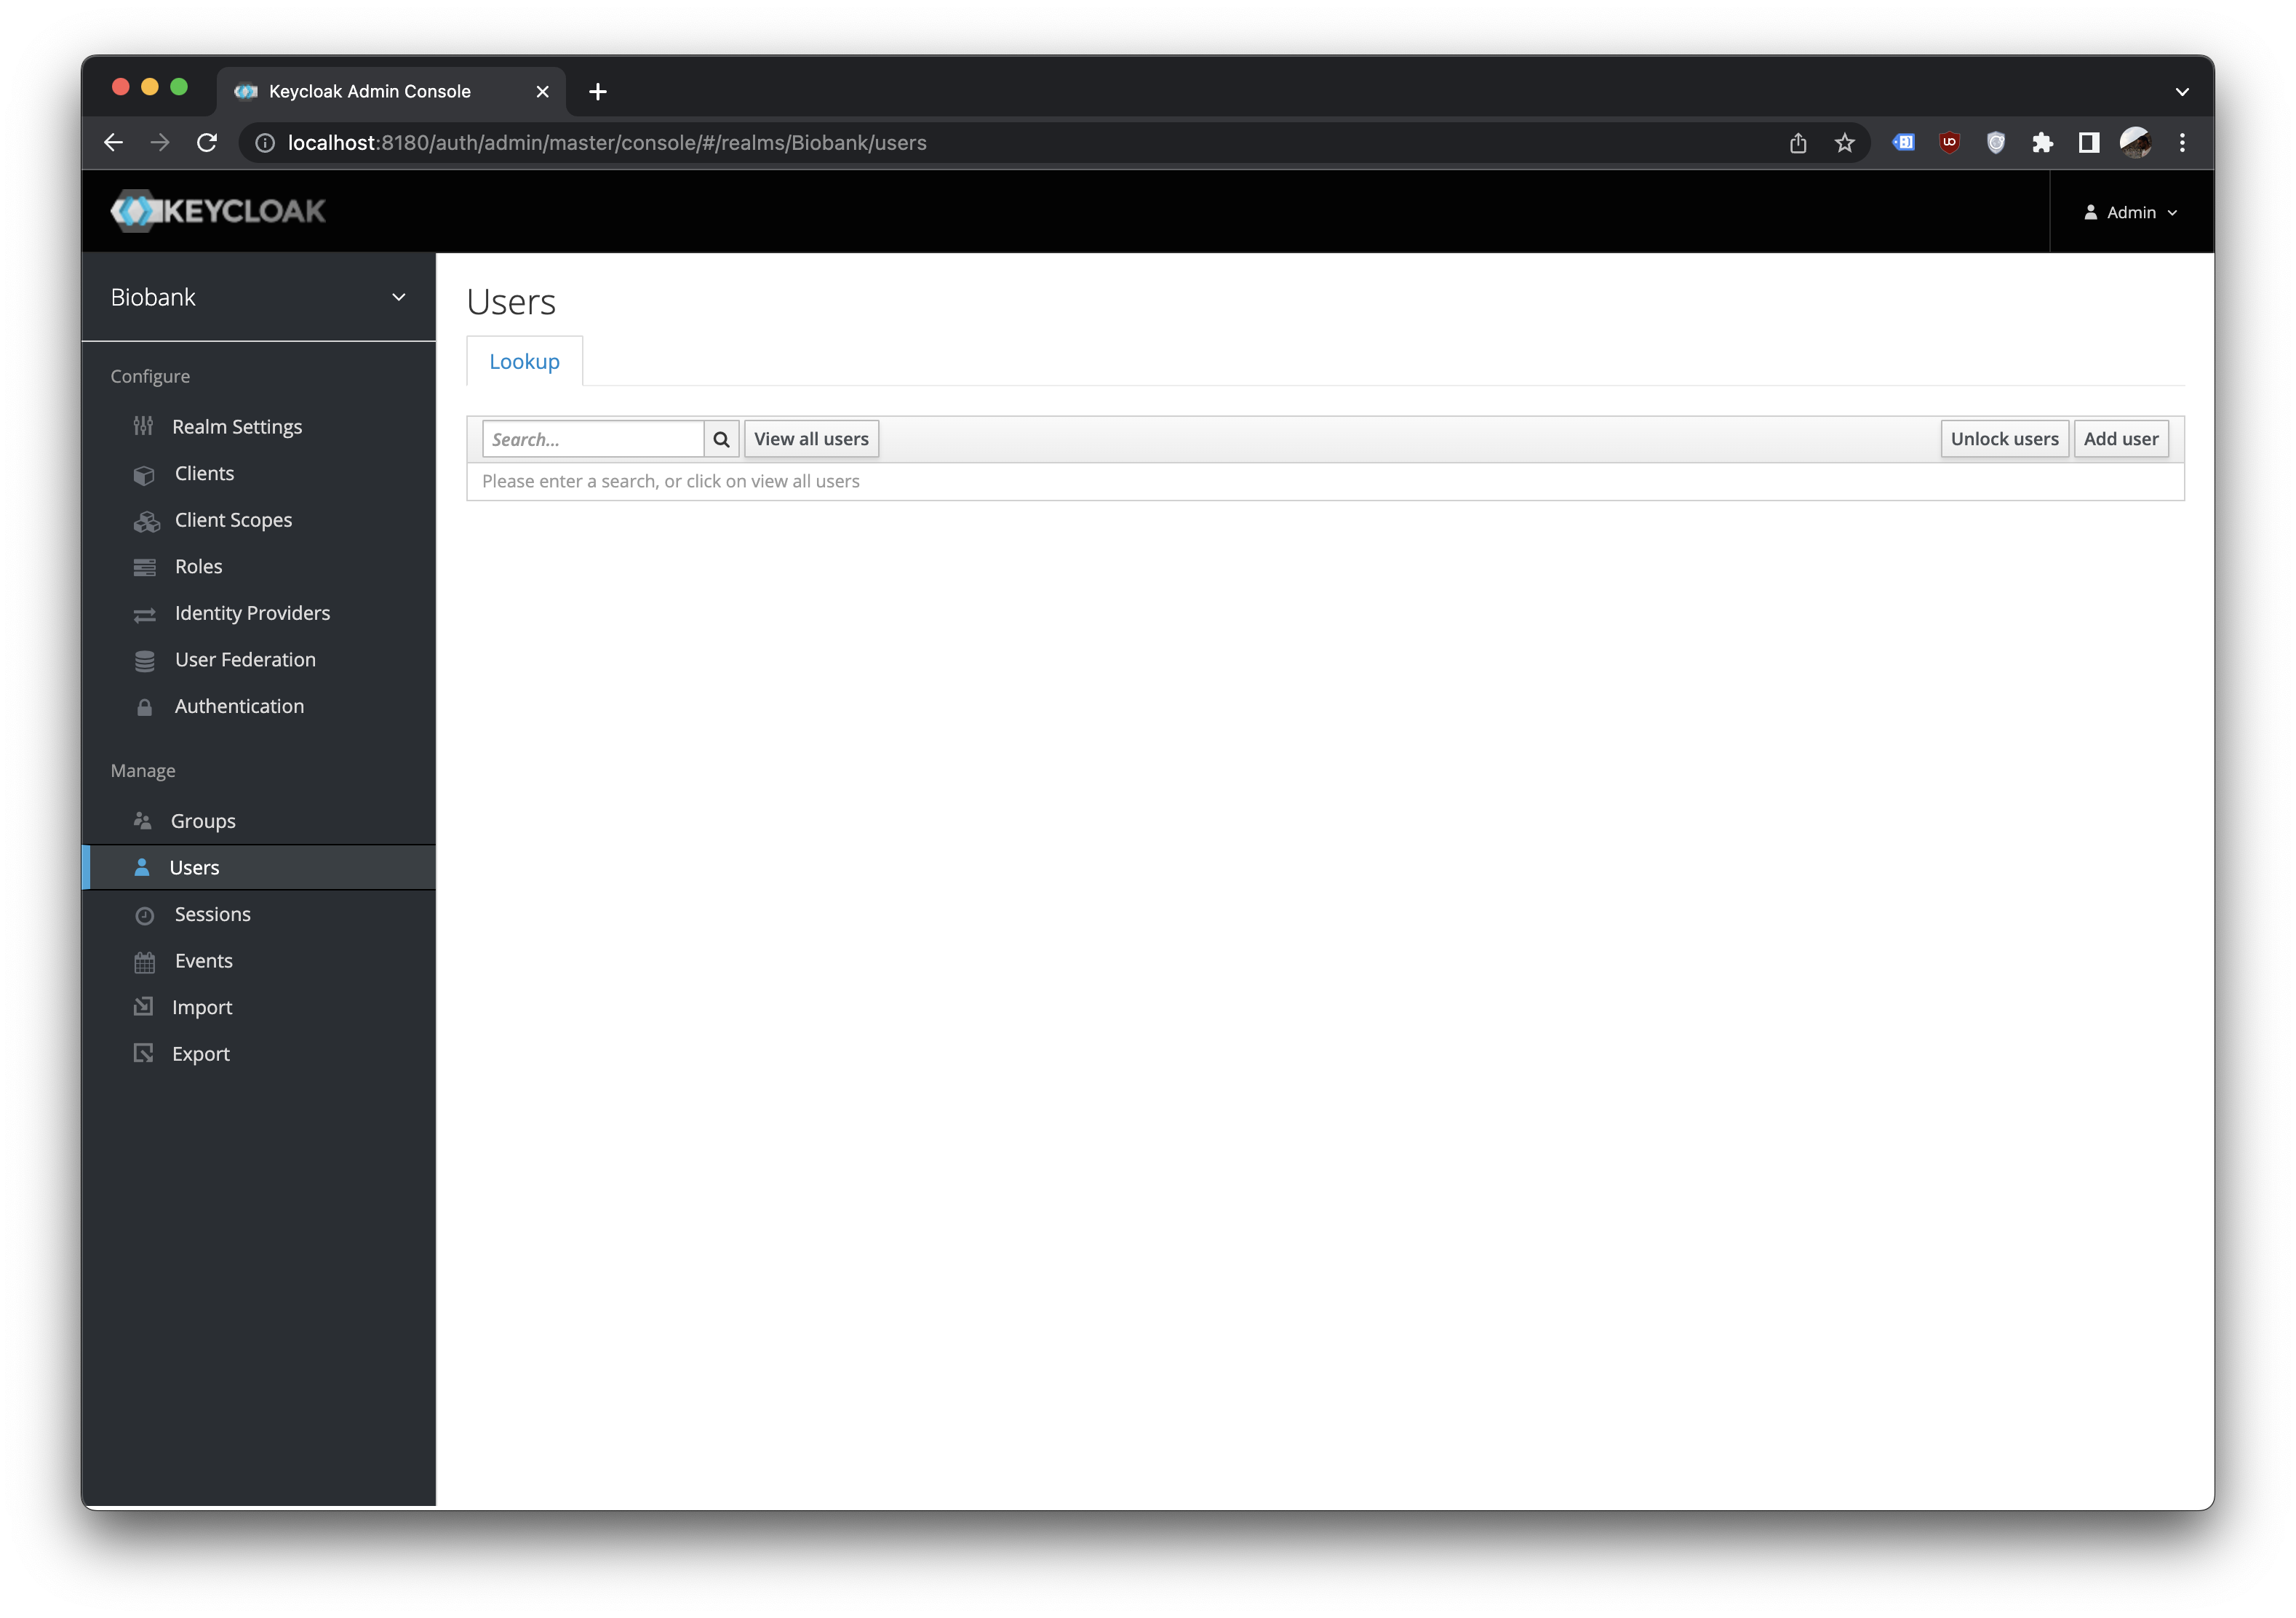
\includegraphics[width=0.80\linewidth]{keycloak_11.png}
\end{center}

Clicchiamo su \textit{Add user}.

\begin{center}
    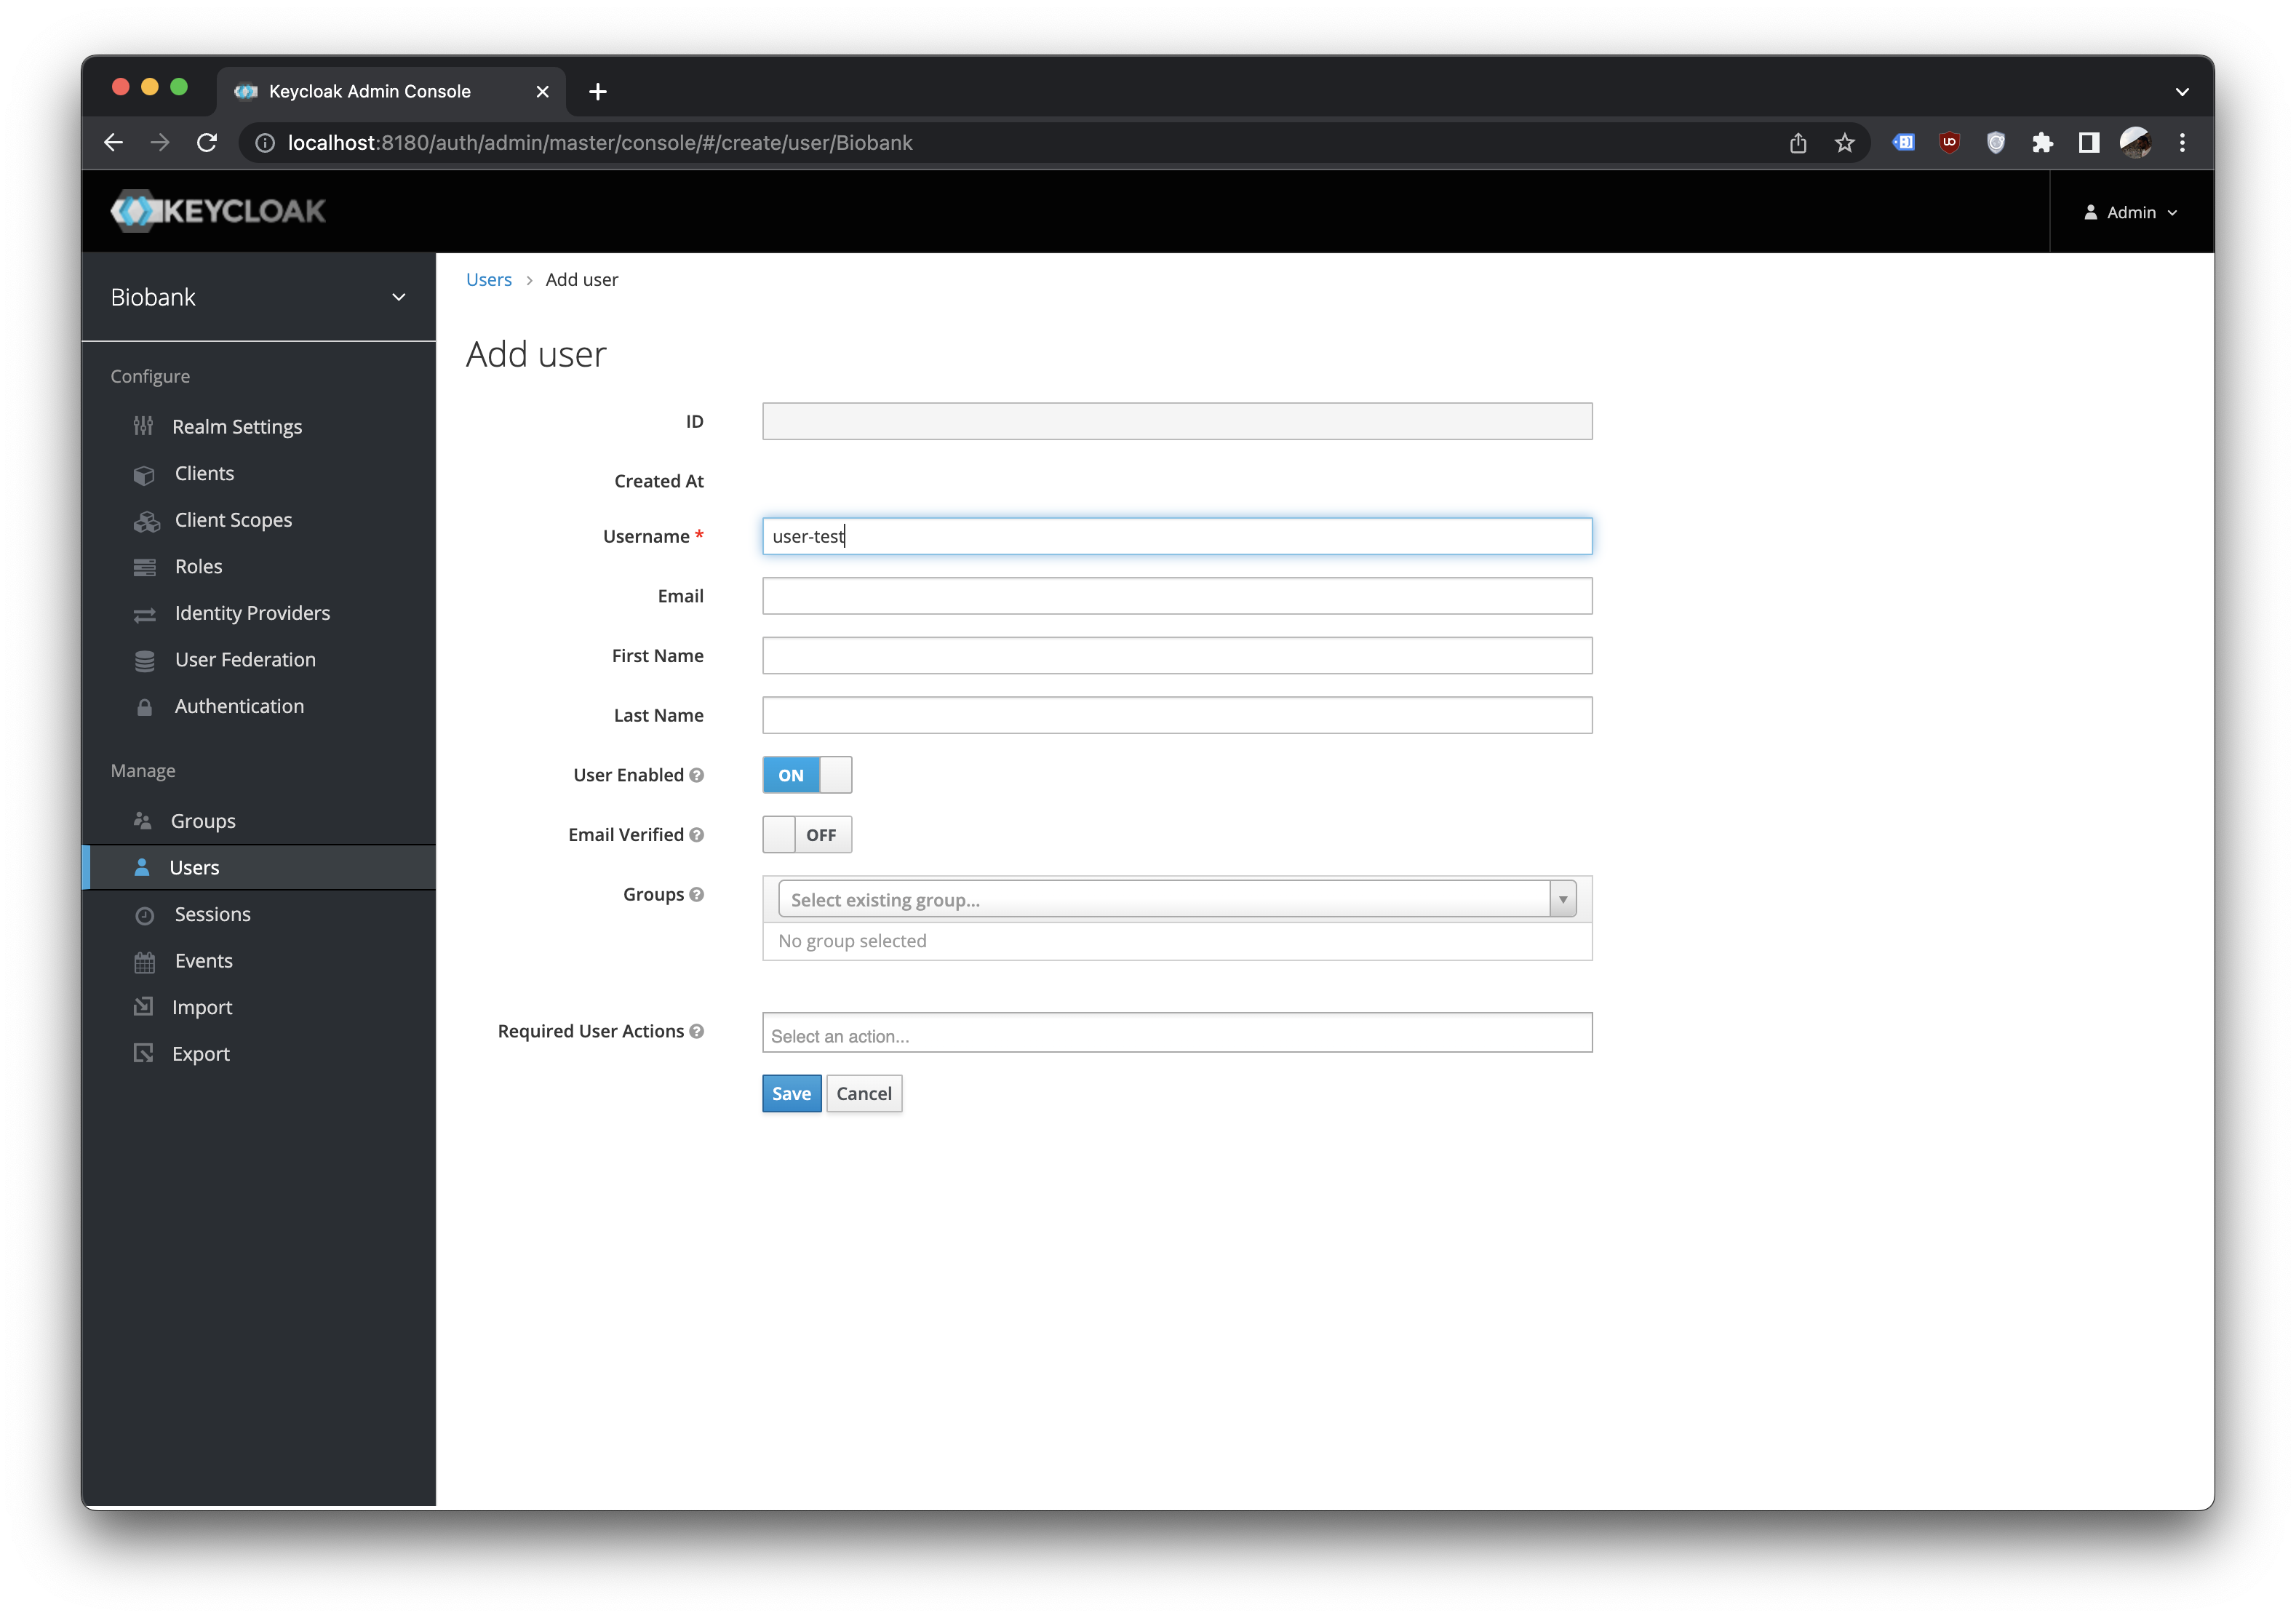
\includegraphics[width=0.80\linewidth]{keycloak_12.png}
\end{center}

Assegniamo un username al nostro utente e clicchiamo su \textit{Save}. La pagina sarà dunque aggiornata con nuovi tab ed opzioni, clicchiamo dunque sul tab \textit{Role Mappings}.
Selezioniamo dunque il client, per il quale vogliamo assegnare un ruolo al nostro utente, dalla select di \textit{Client Roles} e clicchiamo su \textit{Add selected} per assegnargli il ruolo.

\begin{center}
    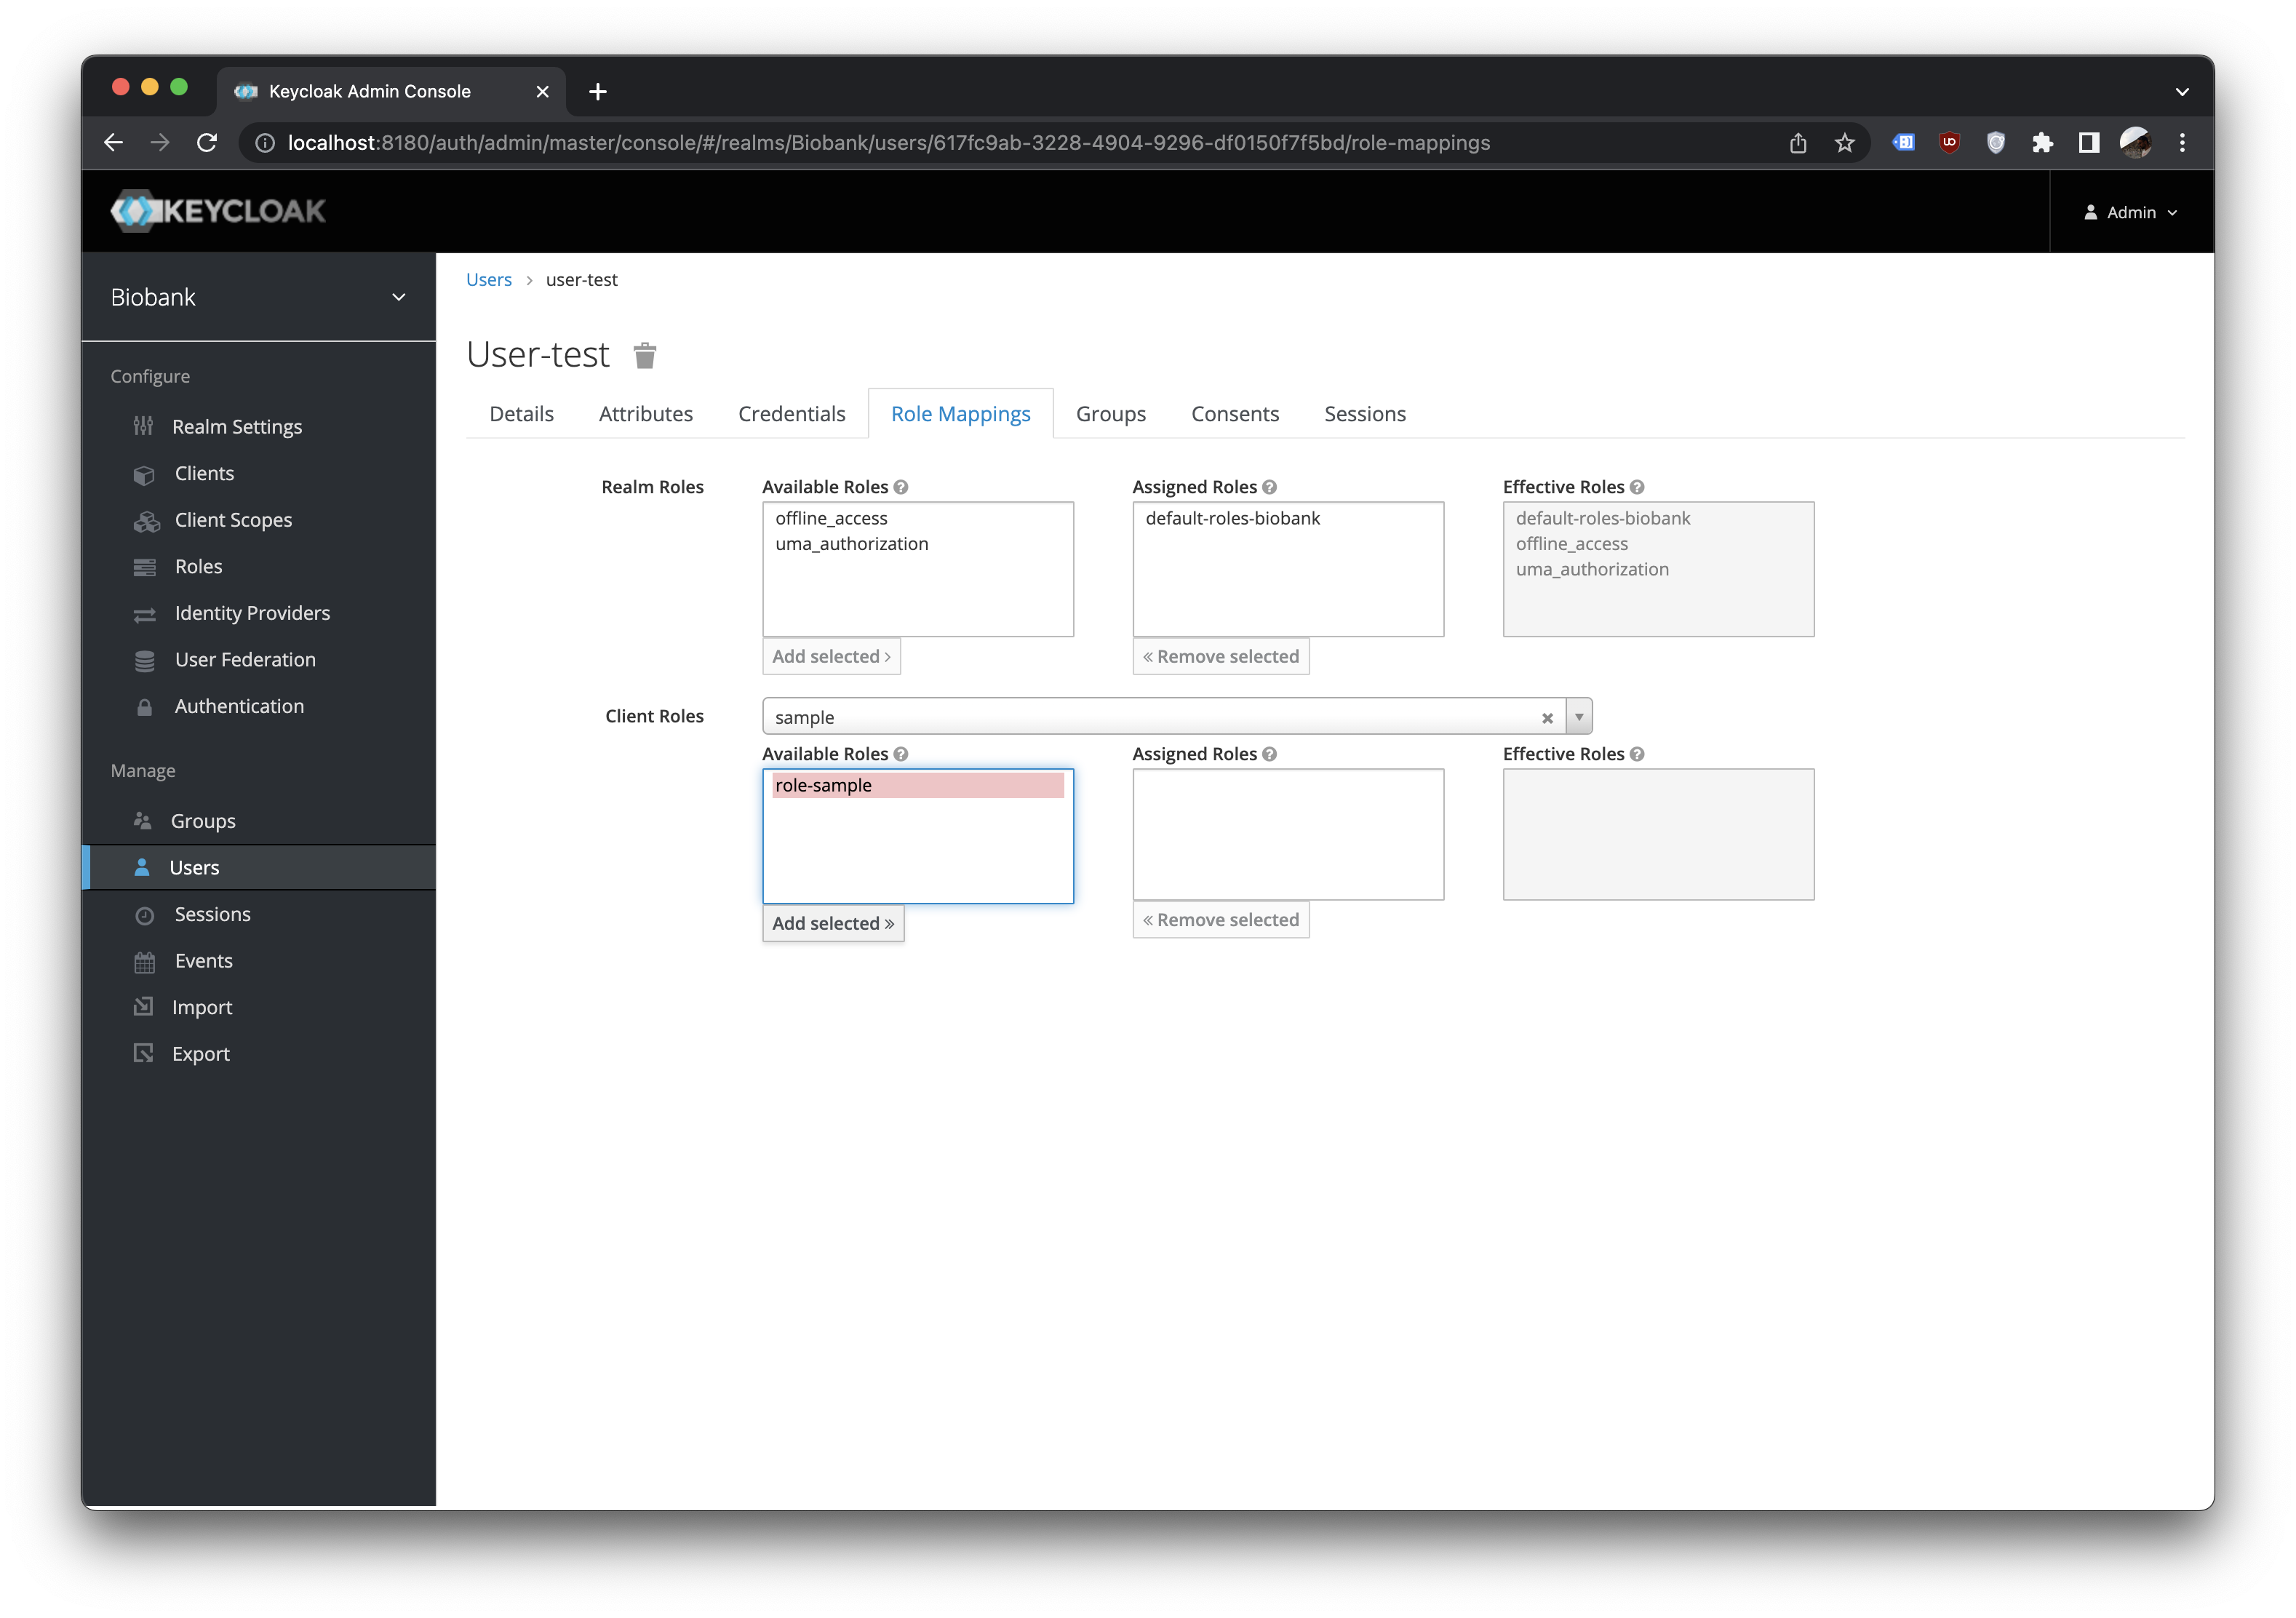
\includegraphics[width=0.80\linewidth]{keycloak_13.png}
\end{center}

Prima di passare allo step successivo, assegniamo una password cliccando sul tab \textit{Credentials} (è possibile assegnare una password temporanea che l'utente potrà cambiare una volta effettuato il primo login).

\begin{center}
    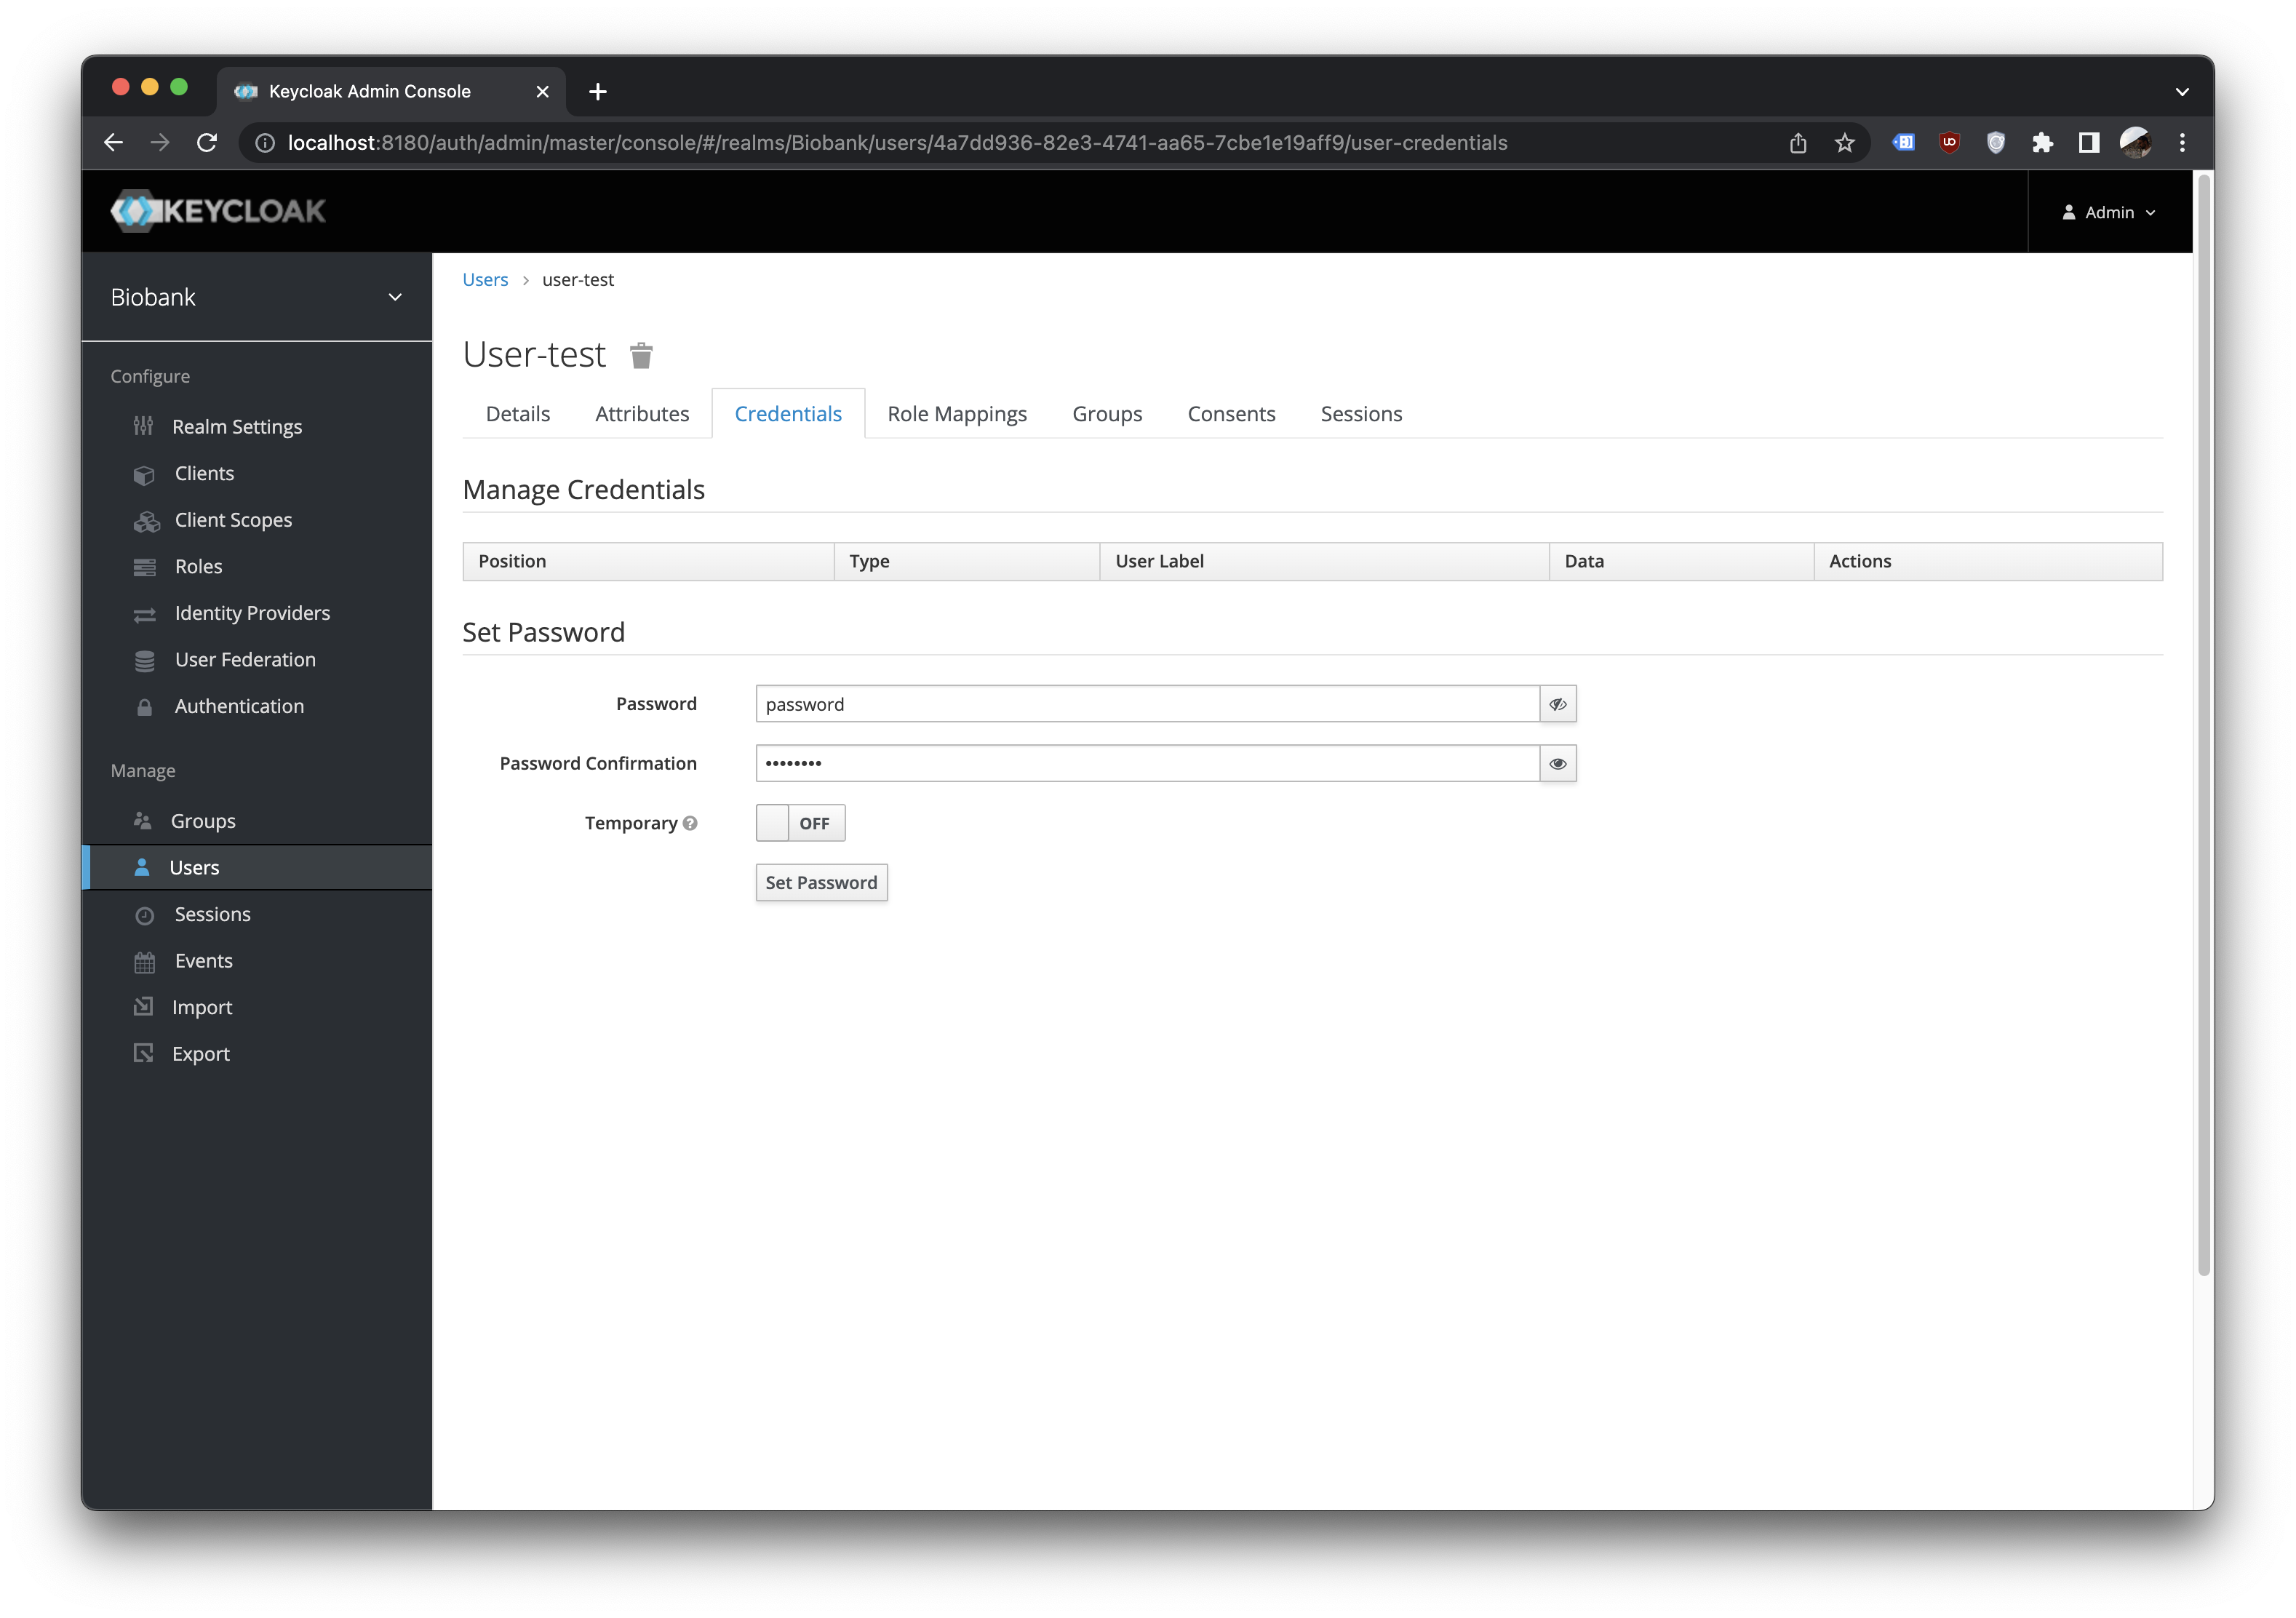
\includegraphics[width=0.80\linewidth]{keycloak_14.png}
\end{center}

\subsection{Dimostrazione autenticazione}

Completati gli step precedenti, adesso siamo pronti ad effettuare un test sull'autenticazione dell'utente.
In questo caso, prenderemo in esame, il microservizio \textit{Sample}. Andando sullo Swagger del relativo microservizio, effettuando una GET su \texttt{/sample/samples}, la richiesta ritornerà \texttt{401 Unauthorized}:

\begin{center}
    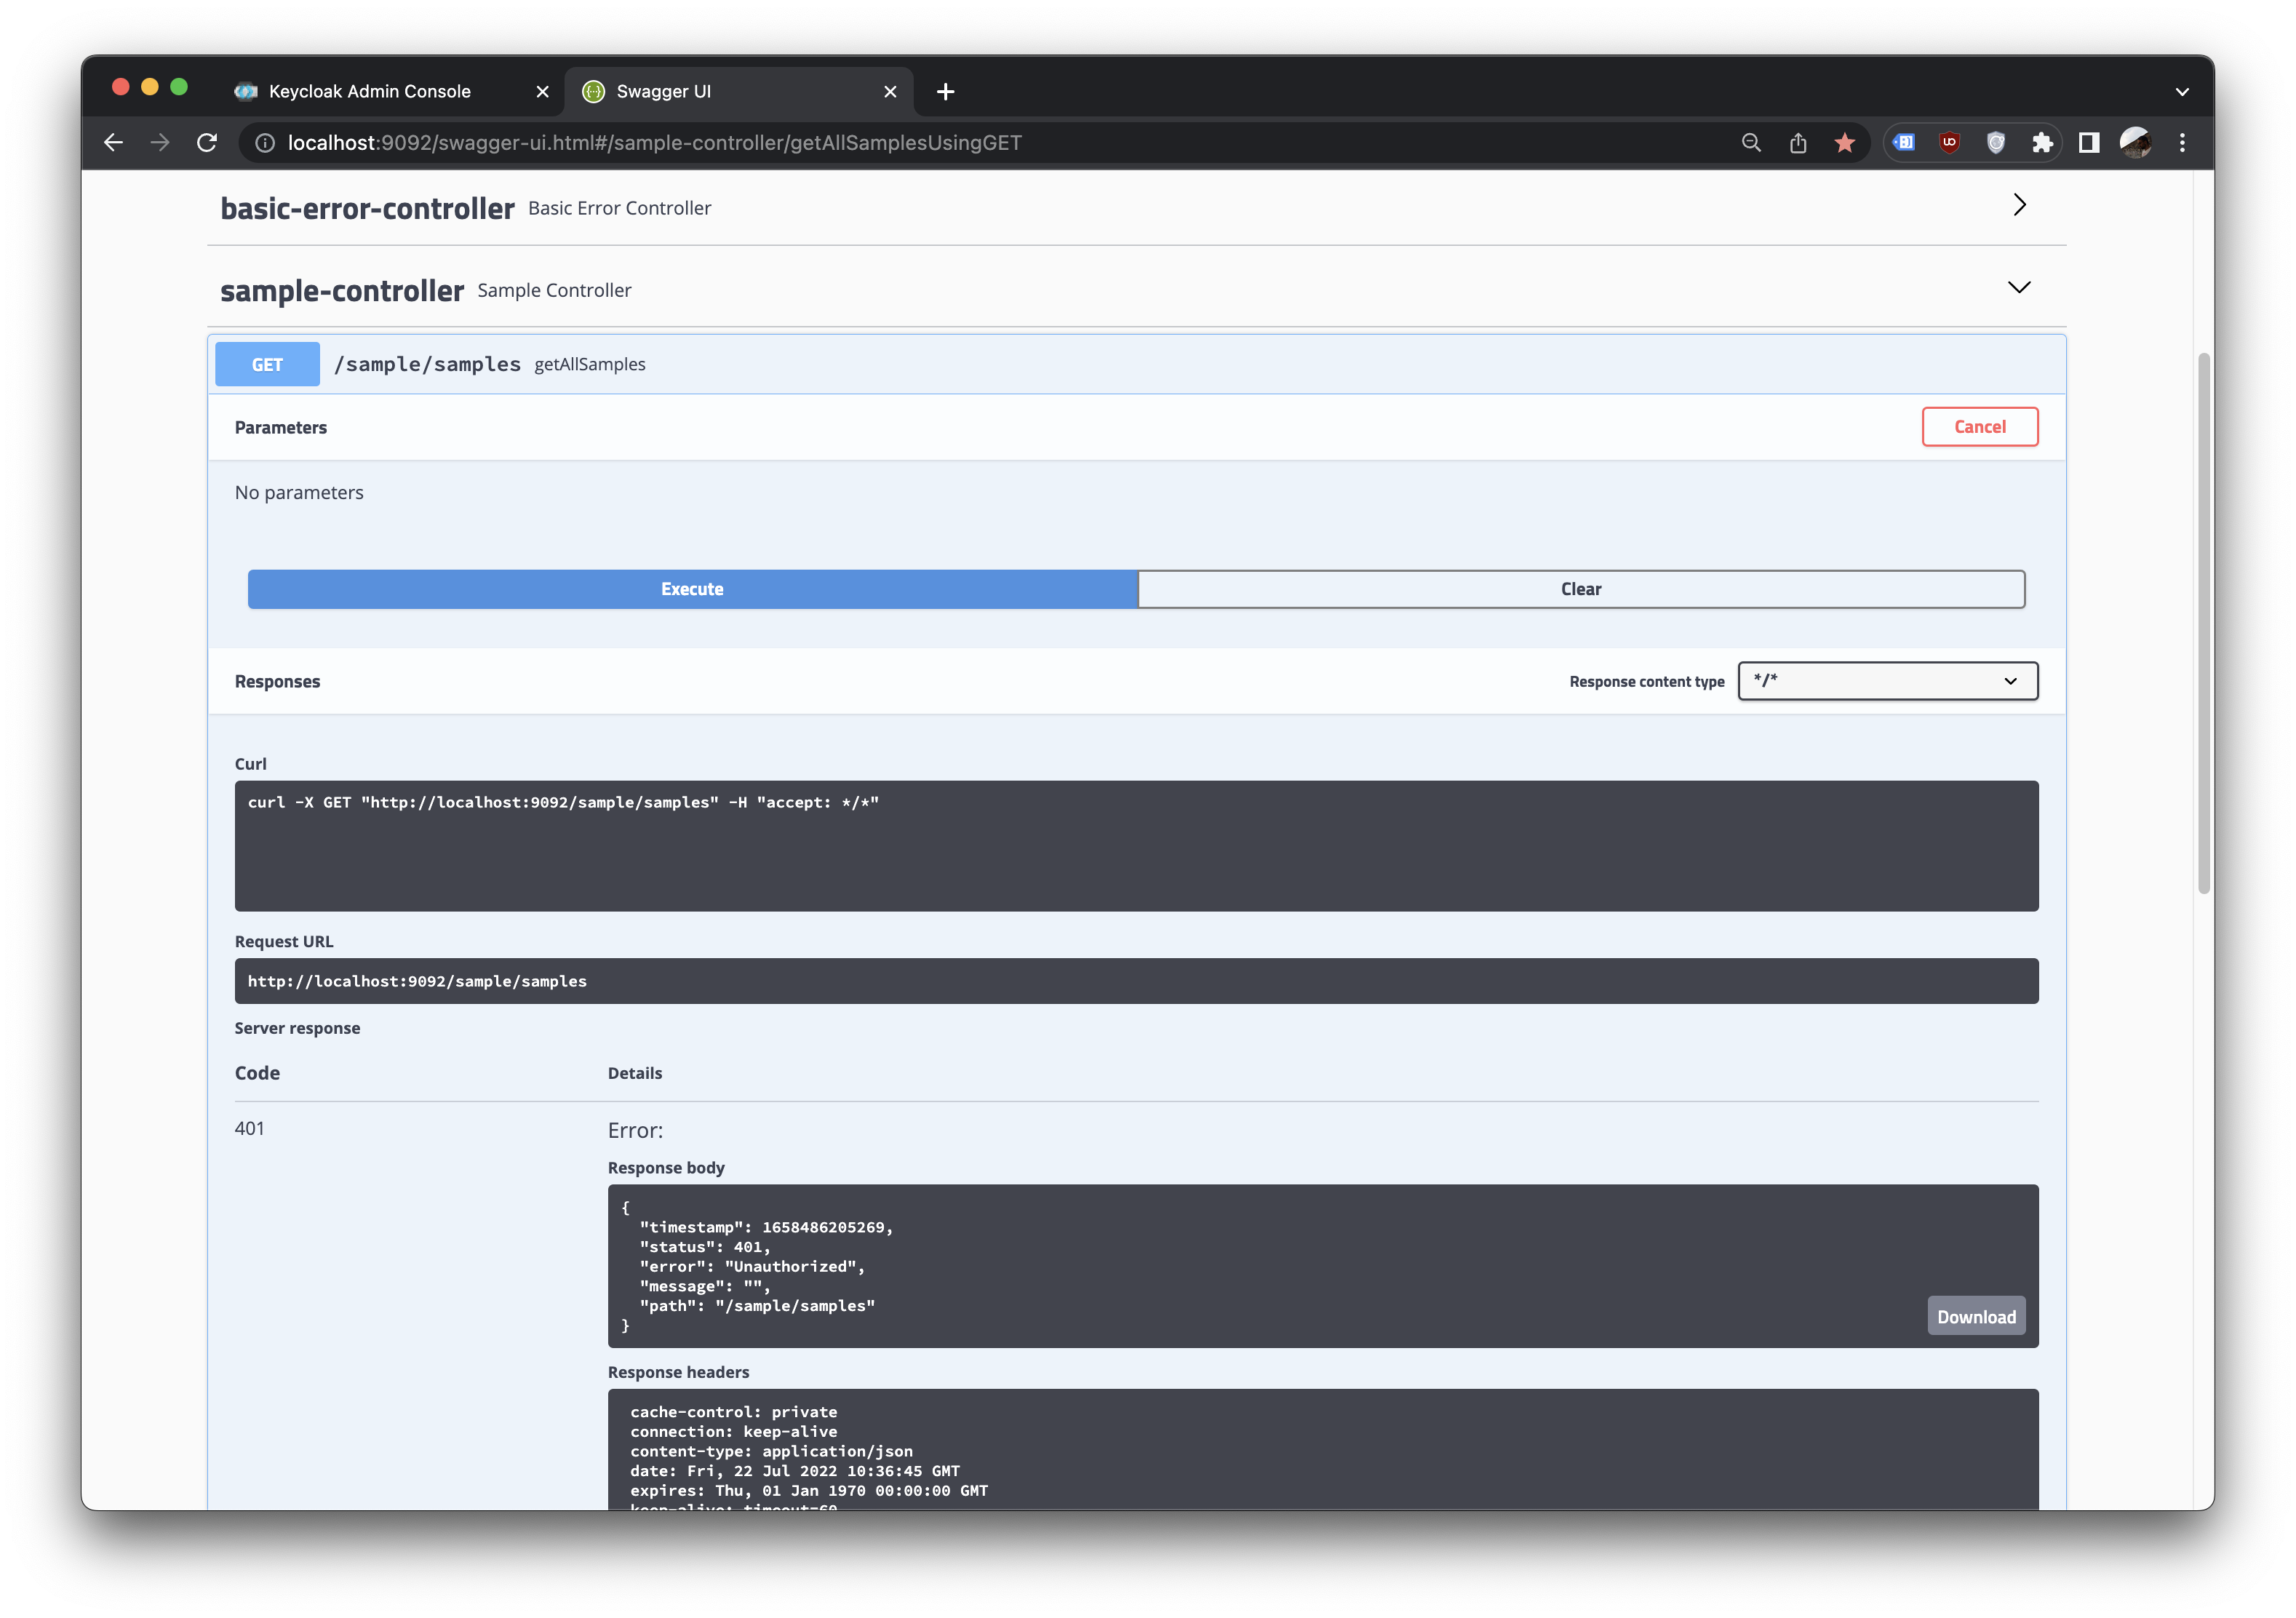
\includegraphics[width=0.80\linewidth]{keycloak_15.png}
\end{center}

Il blocco dell'API funziona correttamente, infatti nelle properties del microservizio sono state settate delle security constraint relative al path \texttt{/sample/*}.

\begin{center}
    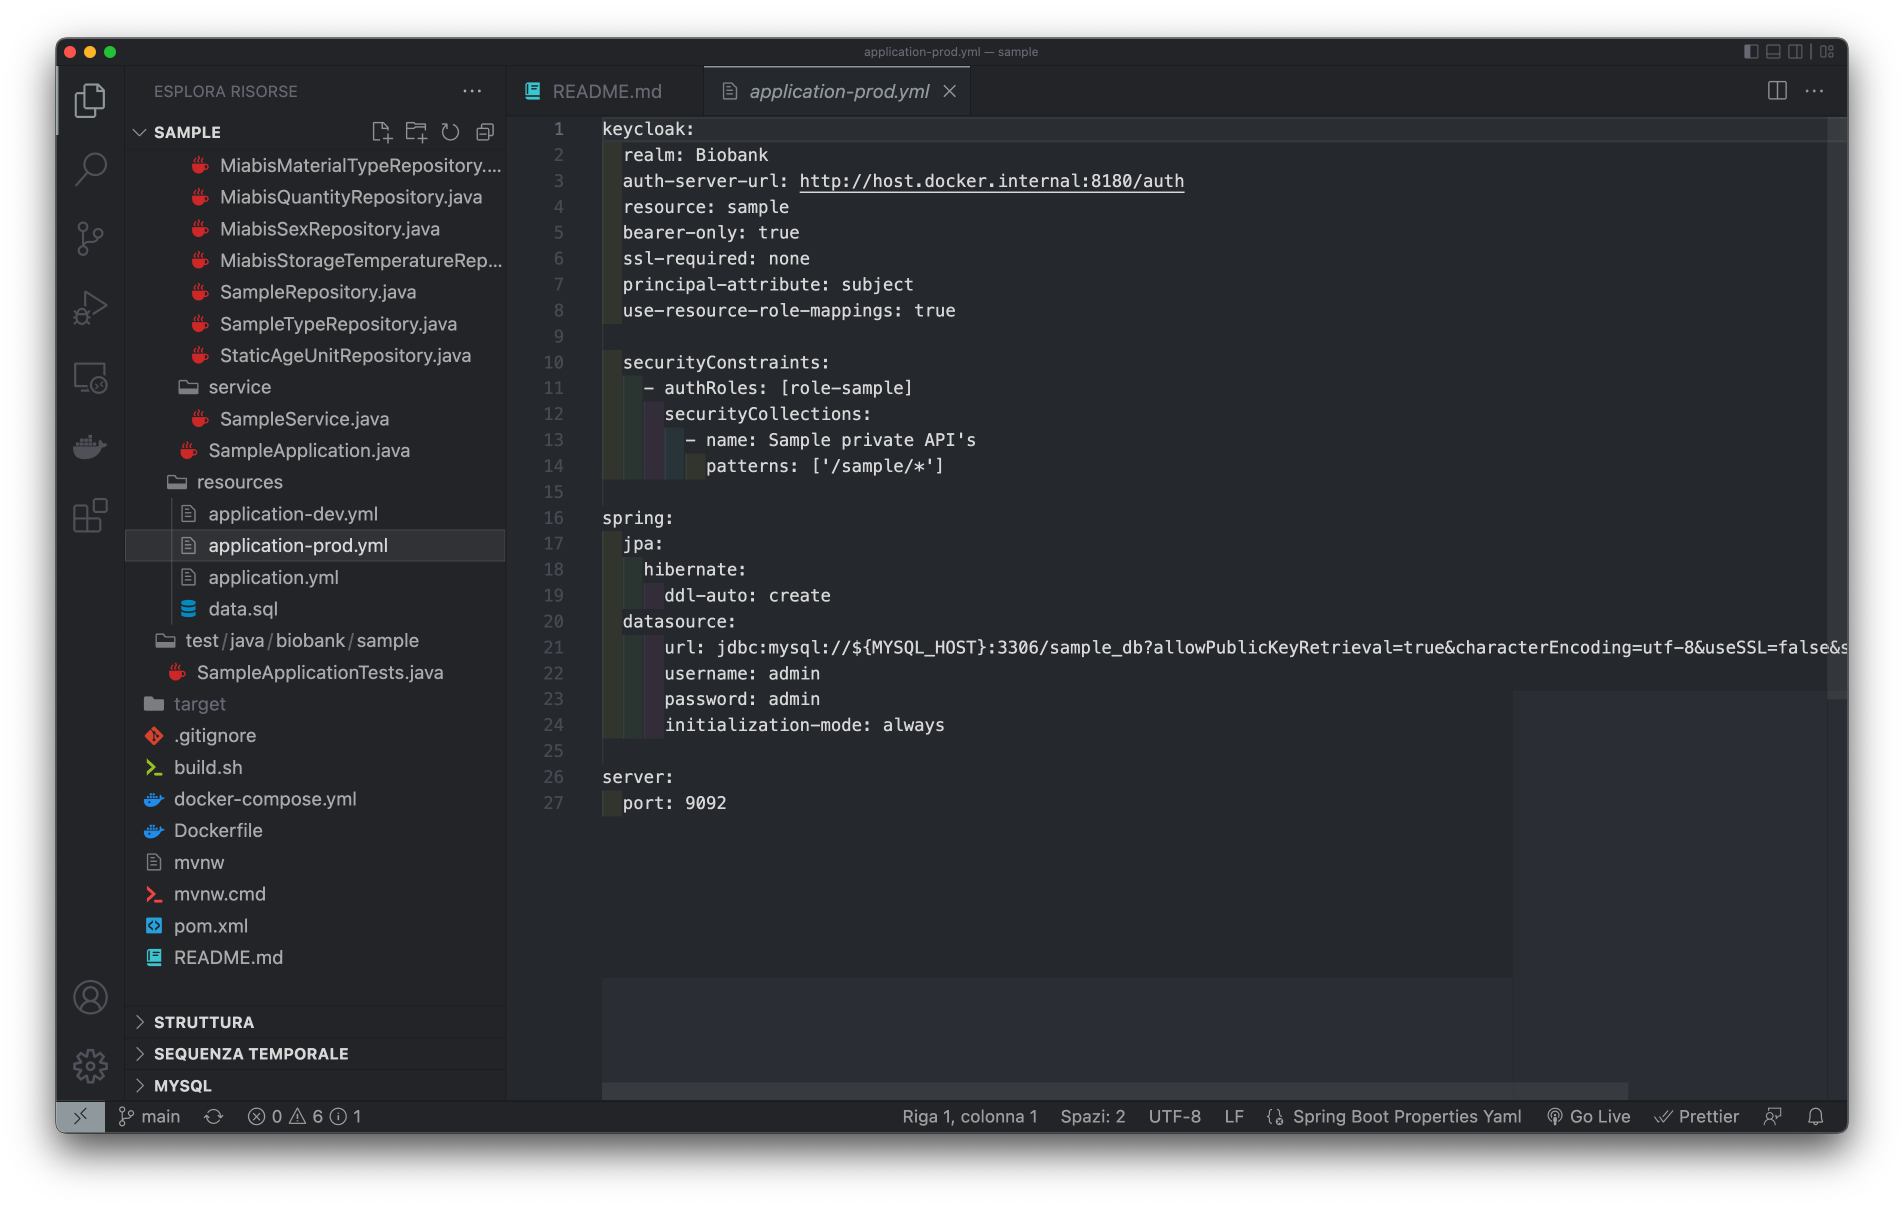
\includegraphics[width=0.80\linewidth]{keycloak_16.png}
\end{center}

Secondo i security constraint, infatti, le API \texttt{/sample/*} possono essere utilizzate solo da un utente che ha assegnato il ruolo \texttt{role-sample} relativo al client \texttt{sample}.

Bisogna effettuare una richiesta a Keycloak con i parametri del nostro utente per avere come ritorno il token \texttt{jwt}.

\begin{verbatim}
    curl --location --request POST 
    'http://localhost:8180/auth/realms/Biobank/protocol/openid-connect/token' \
    --header 'Content-Type: application/x-www-form-urlencoded' \
    --data-urlencode 'client_id=sample' \
    --data-urlencode 'username=user-test' \
    --data-urlencode 'password=password' \
    --data-urlencode 'grant_type=password'
\end{verbatim}

Su \texttt{jwt.io} è possibile visualizzare tutte le informazioni contenute nel token, tra cui il realm di appartenenza ed i ruoli dell'utente:

\begin{center}
    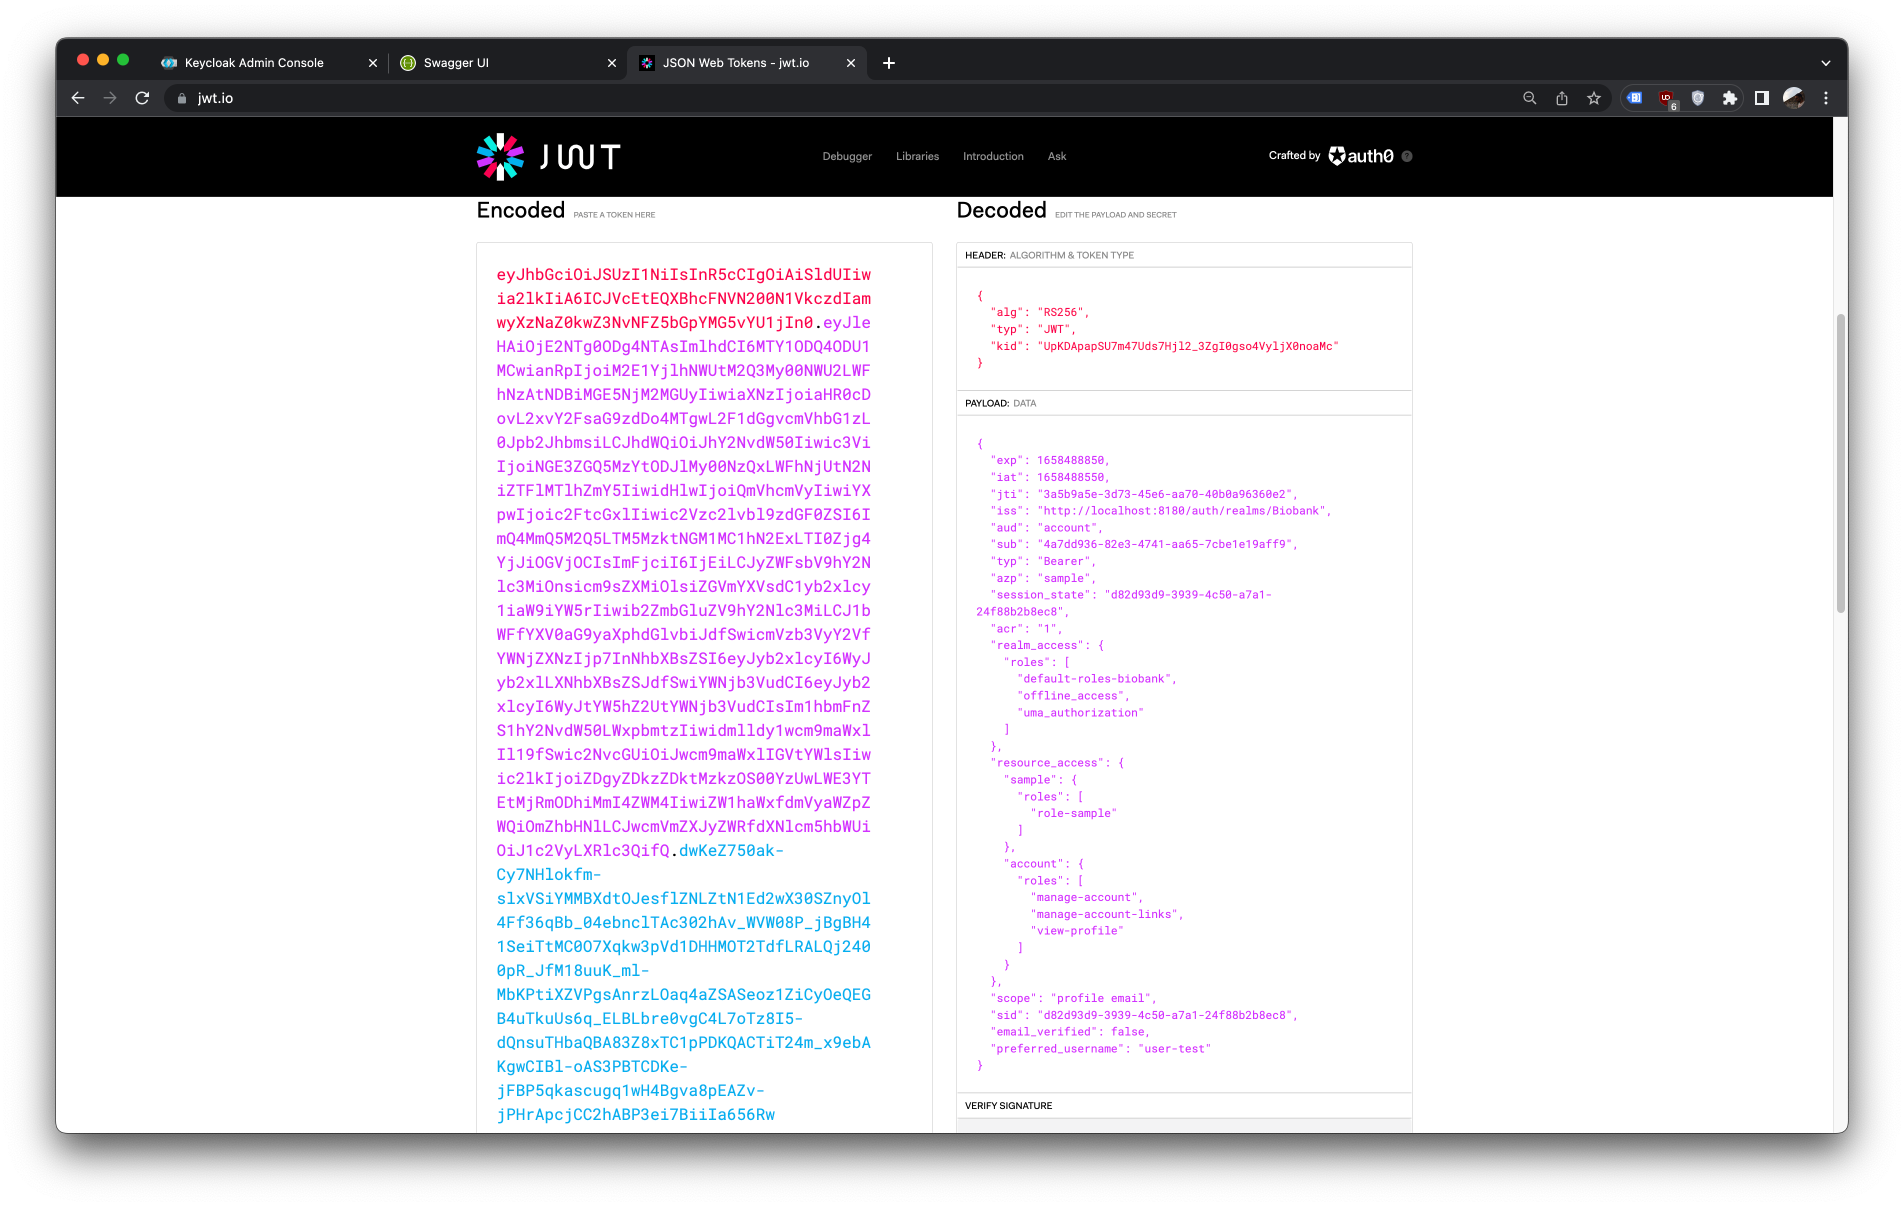
\includegraphics[width=0.80\linewidth]{keycloak_17.png}
\end{center}

Effettuando la medesima chiamata, autenticandoci con token JWT precedentemente generato (in questo caso utilizzeremo POSTMAN), la chiamata andrà a buon fine.

\begin{center}
    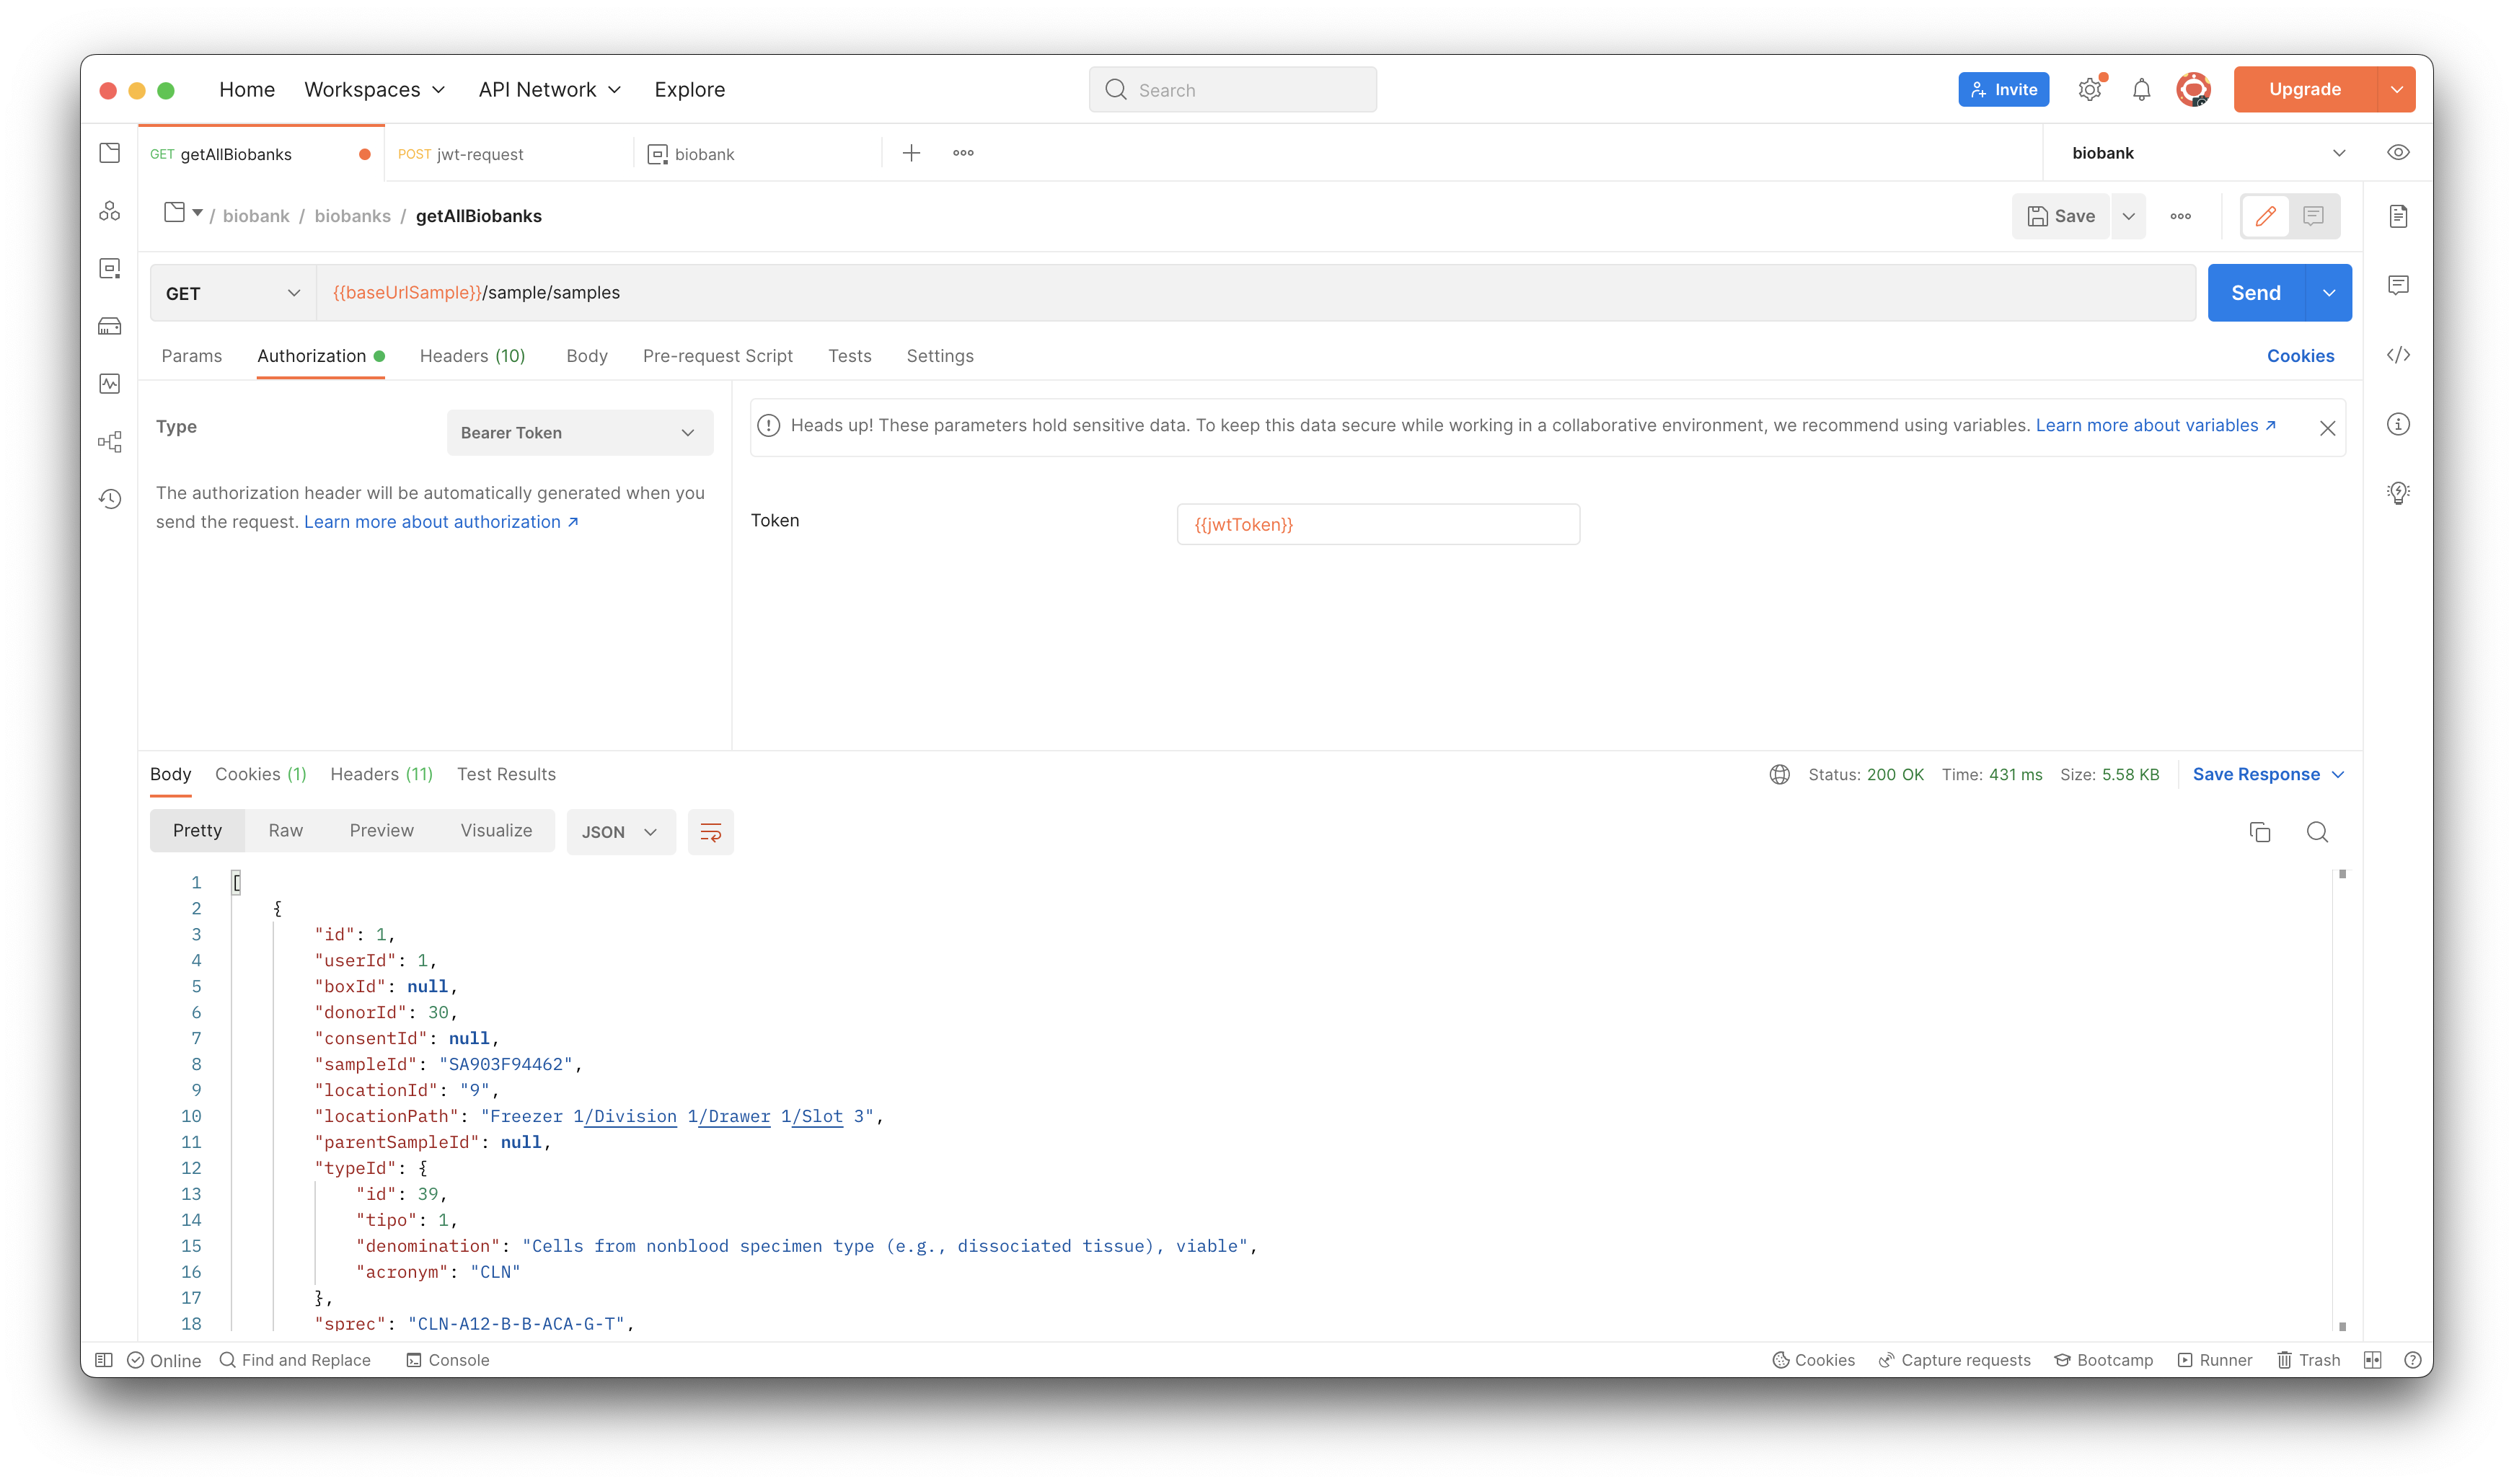
\includegraphics[width=0.80\linewidth]{keycloak_18.png}
\end{center}

Utilizzando un JWT relativo ad un utente con altri ruoli assegnati, ma non quello richiesto dall'API, il messaggio di ritorno è il seguente:

\begin{center}
    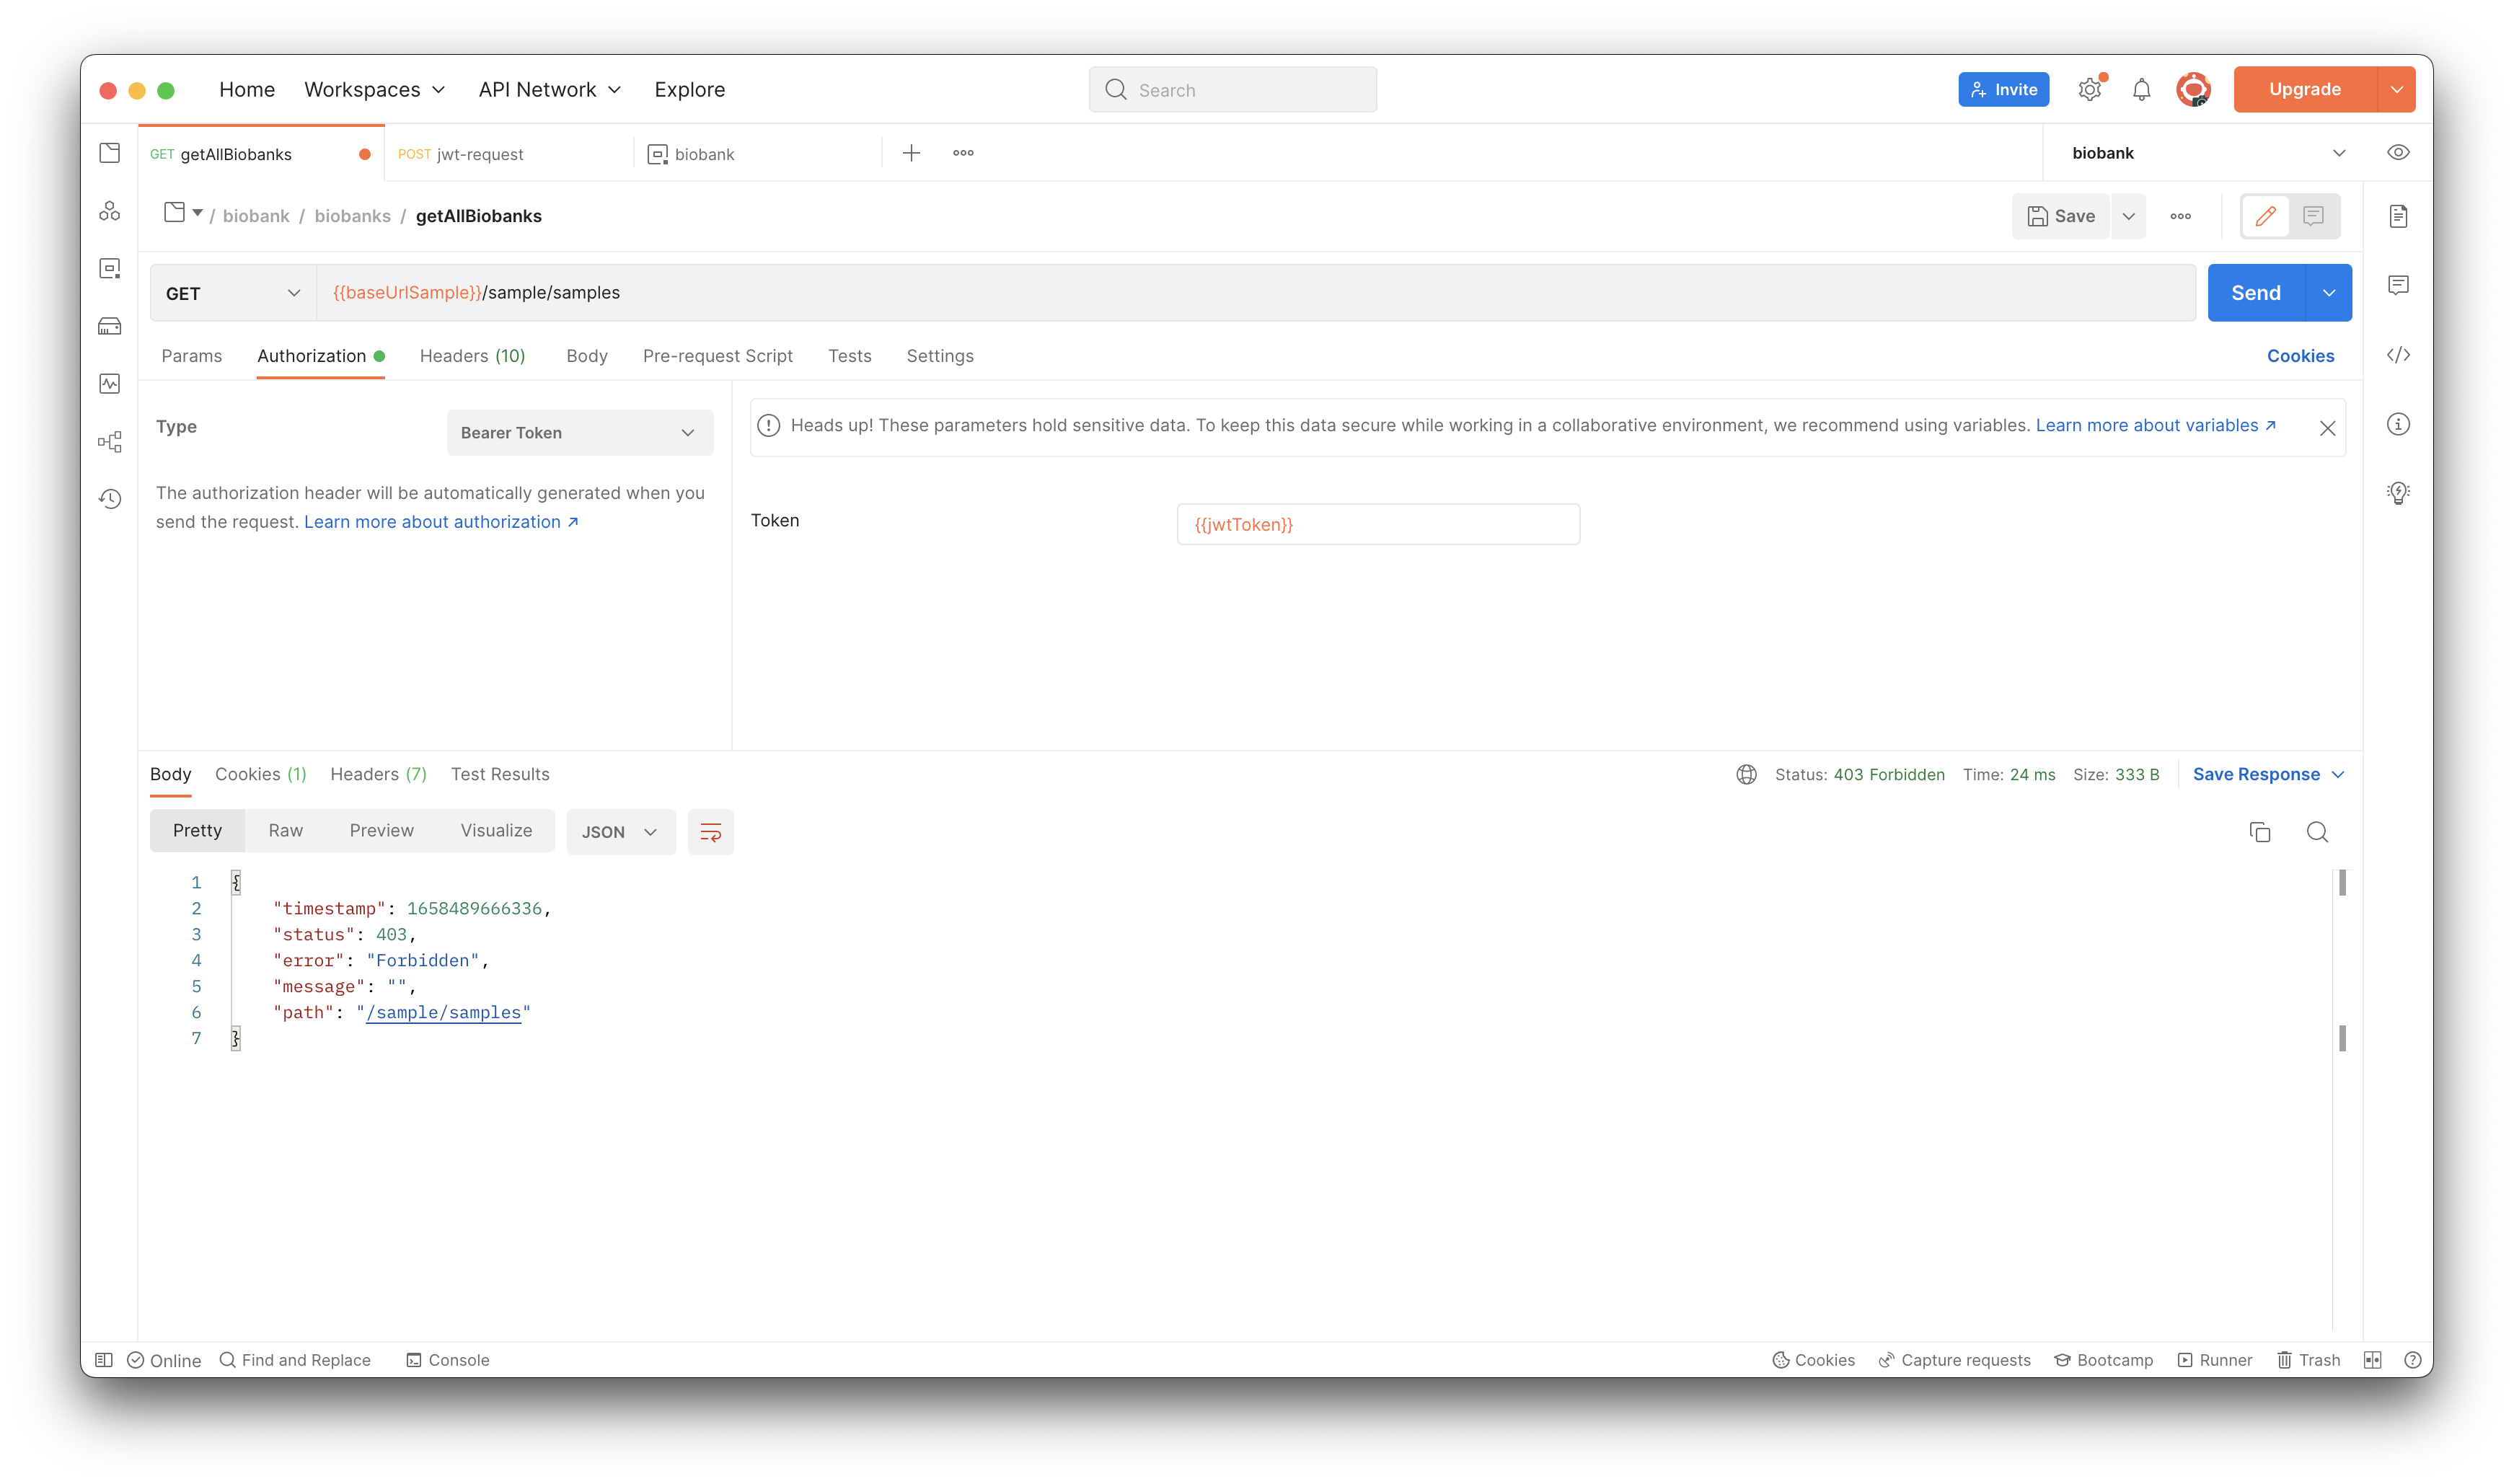
\includegraphics[width=0.80\linewidth]{keycloak_19.png}
\end{center}

Si nota che i messaggi di ritorno possono essere personalizzati in base alle proprie esigenze, in questo caso, è stato ritenuto opprotuno considerare solo il caso base.

\subsection{Conclusione}

La configurazione dell'intero realm \texttt{Biobank} sarà importata automaticamente all'avvio di Keycloak. Oltre ai parametri di configurazione \texttt{application.yaml} è stato necessario importare la classe
\texttt{KeycloakConfig} ed estendere la \texttt{SecurityConfig} con il \texttt{KeycloakWebSecurityConfigurerAdapter}, oltre ad importare la seguente dipendenza sul \texttt{pom.xml}

% TODO: Necessario spiegare che viene implementato nelle securityConfig il KeycloakRestTemplate
% Aggiungere che utilizzandolo in questo modo Shipment e Sample non hanno bisogno di ......

\begin{verbatim}
    <dependency>
        <groupId>org.keycloak</groupId>
        <artifactId>keycloak-spring-boot-starter</artifactId>
    </dependency>
\end{verbatim}

Per ulteriori approfondimenti sugli eventuali utilizzi sono state citate le pagine di documentazione nelle reference a fine relazione.

\pagebreak

\section{Git actions}

Successivamente, è stato ritenuto opportuno ai fini di un buon flusso di sviluppo, integrare delle \textit{git actions} nei vari repository.
Nel dettaglio, è stata implementata una action, denominata \textbf{Create action build and push on Docker Hub} per ogni microservizio, che entra in azione ogni volta che viene effettuato un commit nel 
branch \texttt{main} che. In ordine, gli step sono i seguenti:

\begin{enumerate}
    \item Effettua la build del microservizio utilizzando \texttt{maven};
    \item Crea l'immagine docker del microservizio e la pusha sul repository GitHub
\end{enumerate}

\section{Kubernetes}

TODO: Inserire perché stiamo utilizzando kubernetes


\textit{
Nonostante aver organizzato il flusso di sviluppo, ed in parte quello di deploy, in un ambiente di produzione, è necessario garantire che non si verifichino interruzioni
dei servizi, per esempio, causati dall'interruzione di un container o da un aggiornamento. Nel primo caso, ad esempio, è necessario avviare un nuovo
container. Kubernetes fornisce un framework per far funzionare i sistemi distribuiti in modo resiliente, ad esempio, gestendo
tutti quei comportamenti in maniera automatica. Kubernetes si occupa della scalabilità, failover, distribuzione. 
}


Tra i servizi forniti troviamo:

\begin{enumerate} 
    \item \textbf{Scoperta dei servizi e bilanciamento del carico}: k8s può esporre un container usando un nome DNS o il suo indirizzo IP. Se il traffico verso un container è alto, Kubernetes è in grado di distribuire il traffico su più container in modo che il servizio rimanga stabile;
    \item \textbf{Orchestrazione dello storage}: permette di montare automaticamente un sistema di archiviazione a scelta, come per esempio storage locale, dischi forniti da cloud pubblici e altro ancora;
    \item \textbf{Rollout e rollback automatizzati}: può essere utilizzato per descrivere lo stato desiderato per i propri container e si occuperà inoltre di cambiare lo stato attuale per raggiungere quello desiderato ad una velocità controllata. Per esempio, è possibile automatizzare Kubernetes per creare nuovi container per il tuo servizio, rimuovere i container esistenti e adattare le loro risorse a quelle richieste dal nuovo container;
    \item \textbf{Ottimizzazione dei carichi}: fornisce a Kubernetes un cluster di nodi per eseguire i container. Puoi istruire Kubernetes su quanta CPU e memoria (RAM) ha bisogno ogni singolo container. Kubernetes allocherà i container sui nodi per massimizzare l'uso delle risorse a disposizione;
    \item \textbf{Self-healing}: kubernetes riavvia i container che si bloccano, sostituisce container, termina i container che non rispondono agli health checks, e evita di far arrivare traffico ai container che non sono ancora pronti per rispondere correttamente;
    \item \textbf{Gestione di informazioni sensibili e della configurazione}: kubernetes consente di memorizzare e gestire informazioni sensibili, come le password, i token OAuth e le chiavi SSH. Puoi distribuire e aggiornare le informazioni sensibili e la configurazione dell'applicazione senza dover ricostruire le immagini dei container e senza svelare le informazioni sensibili nella configurazione del tuo sistema;
\end{enumerate}

Per prima cosa, è stata dedicata attenzione alla creazione del db. Come già implementato nel docker-compose,
l’obbiettivo è quello di istanziare dei databases MySQL, indipendenti dal be, con dei dati pre-caricati.
Nel dettaglio, ogni Database è composto da i seguenti volumi di k8s:
\begin{enumerate}
    \item \textbf{ConfigMap} che permette di istanziare il database con i dati e le tabelle selezionate;
    \item \textbf{PersistentVolumeClaim} utilizzato per la persistenza del database;
    \item \textbf{Deployment} che permette di effettuare il deploy dell'immagine e settare le variabili d'ambiente;
    \item \textbf{Service} 
\end{enumerate}

È stato previsto, inoltre, un \textbf{Secret volume} necessario per settare le credenziali di accesso dei database che tuttavia per praticità è stato disabilitato. Per mantenere l'intera infrastruttura
scalabile i database avranno una ed una sola istanza.

Invece, ogni back-end, è composto da un volume di \textit{Deploy} ed un \textit{Service} e 2 repliche.

\textit{TODO: Aggiungi descrizione su come hai messo su keycloak con k8s.....}

% Inserire perché sono stati metti come LoadBalancer solo 2 microservizi
% Inserire motivazione repliche

\section{AWS}

La parte finale, del progetto è stata dedicata per il deploy su aws.
È stato trovato opportuno utilizzare servizio di \textbf{EKS} per gestire il deploy con Kubernetes. Si nota che il \texttt{README} del repository \textit{main},
disponibile al seguente indirizzo \href{https://github.com/sistemi-cloud-2022/main}{https://github.com/sistemi-cloud-2022/main}
è stato ampiamente commentato con tutte le librerie e comandi 
utilizzati per la configurazione ed il set up, di conseguenza alcune procedure saranno omesse.

A differenza dei test effettuati in locale, dove veniva utilizzato il namespace di default, sono stati individuati dei namespace di riferimento per ogni microservizio,
ovvero: \textit{biobank}, \textit{donor}, \textit{sample}, \textit{shipment}, \textit{sprecsample}.  

Inizialmente i primi test sono stati effettuati su \texttt{us-east-1}, tuttavia vista la notevole latenza è stato trovato opportuno settare come regione di default \texttt{eu-central-1}

Dopo aver effettuato il login, come prima cosa si crea il cluster utilizzando una istanza T2 large su dei nodi basati su Linux (l'operazione potrebbe durare più di 20 minuti):

\begin{verbatim}
    eksctl create cluster --name biobank-sprec-v1 --version 1.22 --region eu-central-1 --nodegroup-name linux-nodes --node-type t2.medium --nodes 2
\end{verbatim}

Una volta creato il cluster, basterà eseguire gli script del repository \texttt{main} all'interno della cartella \texttt{k8s}.


\pagebreak

\begin{thebibliography}{4}
    \bibitem{1} \href{https://www.keycloak.org/docs/11.0/getting_started/}{Getting started with Keycloak}
    \bibitem{2} \href{https://www.keycloak.org/docs/latest/server_installation/}{Keycloak server installation}
    \bibitem{3} \href{https://www.keycloak.org/2017/05/easily-secure-your-spring-boot.html}{Easily secure Spring Boot app with Keycloak}
    \bibitem{4} \href{https://www.baeldung.com/spring-boot-keycloak}{Spring boot with keycloak}

\end{thebibliography}


\pagebreak

\end{document}
